\label{Part:paperII}
\renewcommand{\contents}{contents/paperII}%
\begin{pFrontmatter}
    \title{Isogeometric Analysis of Acoustic Scattering using\\Infinite Elements}
	\author[a,$\ast$]{Jon Vegard Ven{\aa}s}%
	\author[a]{Trond Kvamsdal}%
	\author[b]{Trond Jenserud}%
	\address[a]{Department of Mathematical Sciences, Norwegian University of Science and Technology,\\Alfred Getz' vei 1, 7034 Trondheim, Norway}%
	\address[b]{Department of Marine Systems, Norwegian Defence Research Establishment,\\Postboks 115, 3191 Horten, Norway}%
	\eaddress[J.V. Ven{\aa}s]{Jon.Venas@ntnu.no}%
	\eaddress[T. Kvamsdal]{Trond.Kvamsdal@ntnu.no}%
	\eaddress[T. Jenserud]{Trond.Jenserud@ffi.no}%
	\begin{abstract}%
		%Solving scattering problems using numerical steepest descent ... %\cite{Huybrechs2006mah}...
The Kirchhoff approximation yields an accurate approximation of scattering problems on convex rigid bodies for high frequencies. The Kirchhoff--Helmholtz integral has usually been evaluated by discretizing the geometry by triangles, such that the integral may be evaluated exactly. However, this approach has frequency dependent accuracy and frequency dependent memory consumption. In this work, the integrals are evaluated numerically on the exact geometry using the method of numerical steepest descent. Both problems concerning the decreased accuracy and the increased memory consumption for higher frequencies are solved by this approach. The isogeoemtric framework eliminates the tessellation process and enables computations directly on the computer aided design (CAD) model.
	\end{abstract}%
\end{pFrontmatter}

\section{Introduction}
Acoustic scattering by elastic objects is a continuing area of study. Most phenomena in the scattering process can be adequately described by linear elasticity theory, and by further restricting the analysis to homogeneous, isotropic bodies of simple geometries, the mathematical formalism becomes simple enough to be handled by conventional analytic methods. 

The problems fall into mainly three categories: scattering of acoustic waves from elastic objects, scattering of elastic waves from fluid-filled cavities and solid inclusions, and inverse scattering, i.e., obtaining properties of a scattering object from the remotely sensed field. In the first category, the classical problems include scattering by spheres and infinite cylinders: fluid spheres~\cite{Anderson1950ssf}, solid spheres and cylinders~\cite{Faran1951ssb, Anderson1955soa, Hickling1962aoe, Doolittle1968ssb, Flax1978toe, Gaunaurd1983rao}, and spherical and cylindrical shells with various combinations of material properties~\cite{Hickling1964aoe, Doolittle1966ssb, Gaunaurd1987lac, Gaunaurd1991ssb, Kaduchak1998rbm, Chang1994voa, Chang1994soa, Fender1972sfa}. 
Much of the work in this field up to around 1980, is summarized in Flax et al.~\cite{Flax1981pa}.

The surrounding medium is usually considered to be a lossless fluid, but viscous fluids~\cite{Lin1983asb} and viscoelastic media and materials~\cite{Hasheminejad2005asf} are also considered. 

The acoustic illumination is often taken to be a plane wave which is relevant for far-field sources, otherwise point sources are applied in the near-field. For the infinite cylinder, the incident field is in most cases applied normal to the cylinder, but obliquely incident fields are also considered~\cite{Bao1990ras, Daneshjou2017aes}. More recently, the problem of scattering of beams has received much attention~\cite{Marston2007abs, Gong2016aso}. 

Solutions to some non-symmetric problems are also given; e.g. partially fluid filled spheres~\cite{Fawcett2001sfa}, spheres with eccentric cavities~\cite{Hasheminejad2005asf}, and open spheres with internal point sources~\cite{Elias1991sba}.

The studies mentioned above consider a single object in the free field. It is also of interest to study interactions between objects, and between an object and a boundary. The problem of multiple scattering is studied in e.g.~\cite{Gabrielli2001asb} for two elastic spheres, and in~\cite{Wu2006mso} for many fluid spheres, while the scattering by objects close to boundaries, and by  partially buried objects is addressed in~\cite{Zampolli2009bpf}.

Applications of the theory are numerous, and include scattering from marine life~\cite{Stanton1998dbs, Stanton2000asb, Anderson1950ssf}, various aspects of sonar, nondestructive testing, seismology, detection of buried objects~\cite{Sessarego1998sba}, medical imaging~\cite{Wells2006ui}, determination of material properties by inverse scattering~\cite{Ayres1987ias}, and acoustic cloaking. Acoustic cloaking, i.e., making an object acoustically 'invisible', requires acoustic metamaterials and is difficult to realize in practice, but reducing the backscattering strength of an object is an important issue, and can be realized either passively by coating or actively as suggested in e.g. \cite{Avital2015ssa}. 
A recent area of research is noise control in aerospace- and automotive engineering, where sound transmission through cylindrical shells constructed from new composite materials \cite{Talebitooti2016att} and functionally graded materials \cite{Daneshjou2017aes} are studied in order to reduce noise level inside the cabin. The latter problem requires a full 3D solution. %Full 3D, 

The method referred to as classical scattering theory starts with the linearized elasto-dynamic equation of motion (also called Naviers equation). For the intended applications, nonlinear effects are negligible, which justifies the use of the linear approximation. For a certain class of coordinate systems, the field can be expressed in terms of three scalar potentials, which satisfy scalar Helmholtz equations, and admit solutions in the form of infinite series, termed normal modes or partial waves. The formal series expansions contain all the physical features of the solution, i.e., the reflected, transmitted and circumferential (or creeping) waves. The most general problems on finite scatterers in free space are scattering by the spherical shells which requires all three potentials and give solutions in terms of double sums. However, assuming axisymmetric illumination there is no loss of generality in aligning the coordinate axis of the sphere with the axis of the incident field, resulting in an axisymmetric problem. This results in a single infinite series which is much more computational efficient than the general case. This is the approach taken here.
 
%Truncation: 
As the solution is in the form of an infinite series, it needs to be truncated at some point. The summation is terminated when the relative magnitude of the last term is less than some prescribed tolerance, such that no computational parameters are introduced if this tolerance is chosen to be the precision used in the calculations (typically double precision). It is shown, by using symbolic precision in MATLAB, that the computational errors in the implementation are due to round-off errors. This is a natural definition of a computational exact solution.

The work reviewed above solves a host of different problems, and several reference solutions are available, with complexity up to three layers. What the present work provides is the explicit solution for a fully general multilayered sphere, and with corresponding analysis of the computational residual errors. This allows easy design and modeling of reference solutions for the purpose of validating numerical methods.
More specific, the model solves the problem of scattering by an incident plane wave, or wave from a point source, by spherical objects consisting of an arbitrary number of layers. Any combinations of fluid and solid layers can be handled, and the special cases of replacing the Neumann-to-Neumann condition by a single Neumann condition is also included.

An early work on scattering from multilayered spheres and infinite cylinders is Jenserud and Tollefsen~\cite{Jenserud1990ars}. The method employed here is referred to as the global matrix method~\cite{Schmidt1985afw} and is a systematic way of assembling local solutions for the individual layers into a global matrix for the total problem. 
The present work uses the same approach and builds mainly upon the work of Chang and Demkowicz~\cite{Chang1994voa}, which is generalized to multilayered spherical objects.

\begin{figure}
	\centering
	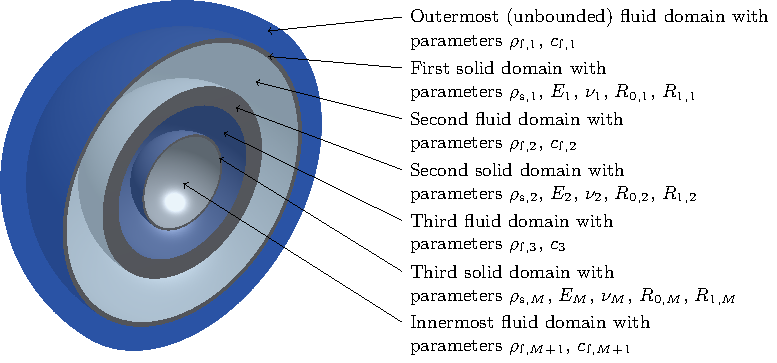
\includegraphics{parameters_distribution}
	\caption{A model with $M=3$ steel shells with different thicknesses (clip view), illustrating the distribution of the physical parameters over the different domains.}
	\label{Fig1:illustration}
\end{figure}
%\clearpage
\newpage
\section{Helmholtz problems}
\label{Sec:exteriorHelmholtz}
Recall that the Helmholtz problem is given by
\begin{alignat}{3}
	\nabla^2 p + k^2 p &= 0 	\quad &&\text{in}\quad \Omega,\label{Eq:HelmholtzEqn}\\
	\partial_n p &= g						&&\text{on}\quad \Gamma,\label{Eq:HelmholtzEqnNeumannCond}
\end{alignat}
where $\partial_n$ denotes the partial derivative in the normal direction, $\vec{n}$, on the surface $\Gamma$. For the exterior problem we must impose the Sommerfeld radiation condition~\cite{Sommerfeld1949pde} 
\begin{equation}\label{Eq:sommerfeldCond}
	\pderiv{p}{r}-\imag k p = o\left(r^{-1}\right)\quad \text{with}\quad r=|\vec{x}|\
\end{equation}
in order to restrict the field in the limit $r\to\infty$ uniformly in $\hat{\vec{x}}=\frac{\vec{x}}{r}$, such that no waves originate from infinity (to obtain uniqueness of the solution $p$).

A common approach for solving unbounded scattering problems with the FEM is to introduce an artificial boundary that encloses the scatterer. On the artificial boundary some sort of absorbing boundary condition (ABC) is prescribed. The problem is then reduced to a finite domain problem, and the bounded domain between the scatterer and the artificial boundary can be discretized with finite elements. Several methods exist for handling the exterior Helmholtz problem (on unbounded domain), including
\begin{itemize}
	\item the infinite element method (IEM)~\cite{Bettess1977ie,Bettess1977dar}
	\item local differential ABC operators~\cite{Shirron1995soe,Bayliss1982bcf,Hagstrom1998afo,Tezaur2001tdf}
	\item the perfectly matched layer (PML)~\cite{Berenger1994apm,Berenger1996pml}
	\item the boundary element method (BEM)~\cite{Sauter2011bem,Schanz2007bea,Marburg2008cao,Chandler_Wilde2012nab}
	\item Dirichlet to Neumann-operators (DtN-operators)~\cite{Givoli2013nmf}.
\end{itemize}
The initial formulation of the IEM assumed the artificial boundary to be a sphere. This restriction results in unnecessary large computational domains for elongated scatterers, and is somewhat relaxed in the ellipsoidal formulation after Burnett~\cite{Burnett1994atd,Burnett1998aea}, in which the infinite elements are attached on an ellipsoid as in~\Cref{Fig:model3_inWaterInf}. These formulations are the ones used in the second paper of this thesis. A further generalization of the artificial boundary was attempted in the work of Shirron and Dey~\cite{Shirron2002aie} where the artificial boundary may be any convex surface. For convex scatterer this enables the infinite elements to be attached directly onto the scatterer as in~\Cref{Fig:model3_in_waterInf2}. It is stated that this infinite element formulation preserves ``the accuracy (and convergence characteristics)'' of the IEM. A statement which can arguably be disputed as illustrated in the appendices as it very much so relies on the geometry of the artificial boundary. However, the reduced computational domain and simpler construction of the artificial boundary may be a sufficient compromise for the accuracy loss. 

\begin{figure}
	\centering
	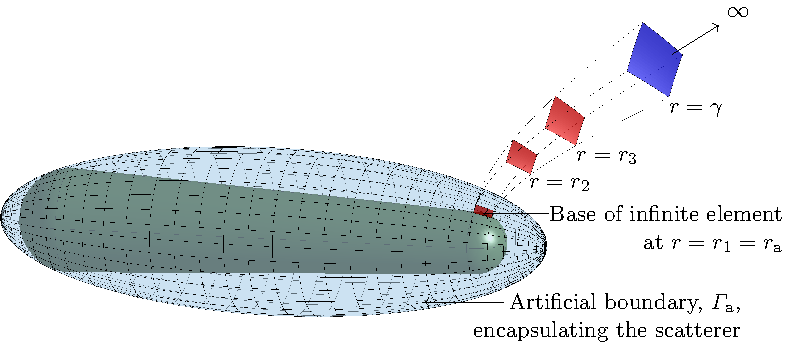
\includegraphics[width=\textwidth]{../../LaTeX/createFigures/TikzFigures/phd/model3_inWaterInf}
	\caption{An infinite element in a prolate spheroidal coordinate system.}
	\label{Fig:model3_inWaterInf}
\end{figure}
\begin{figure}
	\centering
	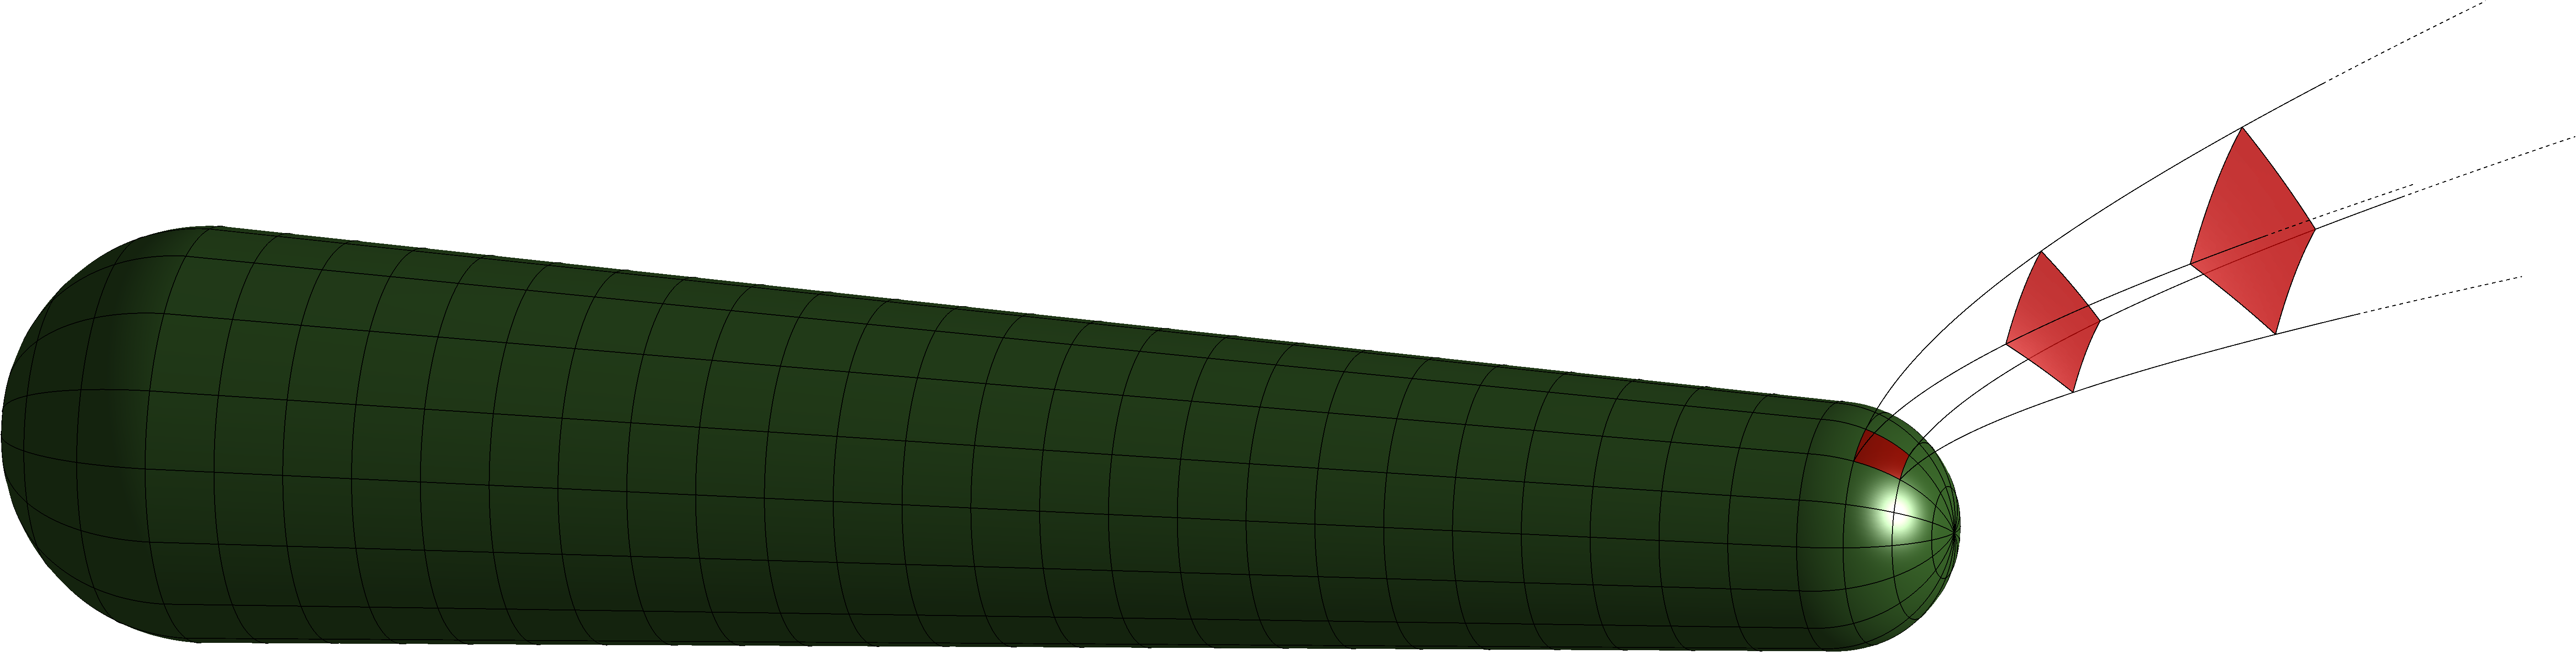
\includegraphics[width=\textwidth]{../../graphics/model3_in_waterInf2}
	\caption{An infinite element attached directly onto the scatterer (which is here the BeTSSi model 3).}
	\label{Fig:model3_in_waterInf2}
\end{figure}

The approach based on ABC operators has developed in much the same way as for the infinite elements with for example an artificial boundary of cigar shape presented in~\cite{Tezaur2001tdf}. Engineering precision ($\sim 1\%$) may be obtained by simple second order operators, but for higher accuracy the formulations becomes arguably more tedious to implement compared to the IEM as higher order derivatives are required. On the other hand, the conditioning of the system matrices for this approach is better than that of the infinite element method. Several attempts have been presented for the IEM to resolve the conditioning problem including~\cite{Dreyer2003ico,Safjan2001tic,Safjan2002tdi}. In~\cite{Safjan2002tdi} Safjan and Newman present basis functions with compact support (in the radial direction) also outside of the artificial boundary. Combining this approach with that of Shirron and Dey would be an approach to solve the conditioning problem while at the same time having lots of freedom to construct the artificial boundary.

The problems outlined above are not present for the BEM approach. Additionally BEM comes with several advantages including reduction of problem dimension (3D volume to 3D surface), no need to do surface-to-volume parametrization (thus, especially suited for IGA), and automatic incorporation of the Sommerfeld radiation condition. However, a host of new challenges arises. This includes fictitious eigenfrequencies, singular integrals and fully dense system matrices. All of which are presented in the third paper.

\subsection{Far field pattern}
The target strength (the quantity of interest) is defined in the far field and we are only solving for the near field. The Helmholtz integral equation gives us a convenient way to link these two fields.

If the field at the scatterer is known (i.e. after obtaining the solution numerically), one can compute the solution in the exterior domain, $\Omega^+$, using the following integral equation (cf.~\cite[Theorem 2.21]{Chandler_Wilde2012nab})
\begin{equation}\label{Eq:KirchhoffIntegral}
	p(\vec{x}) = \int_{\Gamma}\left[ p(\vec{y})\pderiv{\Phi_k(\vec{x},\vec{y})}{n(\vec{y})} - \Phi_k(\vec{x},\vec{y})\pderiv{p(\vec{y})}{n(\vec{y})}\right]\idiff \Gamma(\vec{y}),\quad\vec{x}\in\Omega^+
\end{equation}
where $\vec{y}$ is a point on the surface $\Gamma$, $\vec{n}$ lies on $\Gamma$ pointing ``into'' $\Omega^+$ at $\vec{y}$, and $\Phi_k$ is the free space Green's function for the Helmholtz equation in \Cref{Eq:HelmholtzEqn} given (in 3D) by
\begin{equation}\label{Eq:FreeSpaceGrensFunction}
	\Phi_k(\vec{x},\vec{y}) = \frac{\euler^{\imag kR}}{4\PI R},\quad\text{where}\quad R = |\vec{x} - \vec{y}|
\end{equation} 
with
\begin{equation*}
	\pderiv{\Phi_k(\vec{x},\vec{y})}{n(\vec{y})} = \frac{\Phi_k(\vec{x},\vec{y})}{R}(\imag kR-1)\pderiv{R}{n(\vec{y})}.
\end{equation*}
Using the limits (with $\vec{x}=\hat{\vec{x}}/r$ and $r=|\vec{x}|$)
\begin{equation}\label{Eq:Phi_k_limits}
\begin{aligned}
	&\lim_{r\to\infty} r\euler^{-\imag k r}\Phi_k(r\hat{\vec{x}},\vec{y}) = \frac{1}{4\PI}\euler^{-\imag k \hat{\vec{x}}\cdot\vec{y}}\\
	&\lim_{r\to\infty} r\euler^{-\imag k r}\pderiv{\Phi_k(r\hat{\vec{x}},\vec{y})}{n(\vec{y})} = -\frac{\imag k}{4\PI}\euler^{-\imag k \hat{\vec{x}}\cdot\vec{y}}\hat{\vec{x}}\cdot\vec{n}(\vec{y})
\end{aligned}
\end{equation}
the formula in \Cref{Eq:KirchhoffIntegral} simplifies in the far field to (cf.~\cite[p. 32]{Ihlenburg1998fea})
\begin{equation}\label{Eq:HelmholtzIntegralFarField}
	p_0(\hat{\vec{x}}) = -\frac{1}{4\PI}\int_{\Gamma}\left[ \imag k p(\vec{y})\hat{\vec{x}}\cdot\vec{n}(\vec{y}) + \pderiv{p(\vec{y})}{n(\vec{y})}\right]\euler^{-\imag k \hat{\vec{x}}\cdot\vec{y}}\idiff \Gamma(\vec{y}).
\end{equation}
from which the target strength in~\Cref{Eq:TS} may be computed.

%
%\subsection{Absorbing boundary conditions}
%\textcolor{red}{Give introduction to ABC and numerical example.}
%
%The ABC operator of first order is given by
%\begin{equation*}
%	\pderiv{u}{r} = \left(\imag k - \frac{1}{r_{\mathrm{a}}}\right) u 
%\end{equation*}
%and the second order operator by
%\begin{equation*}
%	\pderiv{u}{r} = \left(\imag k-\frac{1}{r_{\mathrm{a}}}\right) u + \frac{1}{2r_{\mathrm{a}}}\frac{1}{1-\imag kr_{\mathrm{a}}}\nabla_{\mathrm{S}}^2 u
%\end{equation*}
%the third is given by
%\begin{equation*}
%	\pderiv{u}{r} = \left(\imag k - \frac{1}{r_{\mathrm{a}}}\right) u + \frac{1}{2r_{\mathrm{a}}}\frac{1}{1-\imag kr_{\mathrm{a}}}\nabla_{\mathrm{S}}^2 u + \frac{1}{2}\frac{1}{1-\imag kr_{\mathrm{a}}}\frac{1}{2-\imag k r_{\mathrm{a}}}\left(2+\nabla_{\mathrm{S}}^2\right)\left[\left(\frac{1}{r_{\mathrm{a}}}-\imag k\right)u+\pderiv{u}{r}\right]
%\end{equation*}
%with
%\begin{equation*}
%	\nabla_{\mathrm{S}}^2 = \pderiv[2]{}{\vartheta} + \cot\vartheta\pderiv{}{\vartheta} + \frac{1}{\sin^2\vartheta}\pderiv[2]{}{\varphi}
%\end{equation*}
%
%Since (for the second order operator)
%\begin{equation*}
%	-\int_{\Gamma_{\mathrm{a}}} q\nabla p\cdot\vec{n}\idiff\Gamma = -\int_{\Gamma_{\mathrm{a}}} q\pderiv{p}{r}\idiff\Gamma = -\left(\imag k-\frac{1}{r_{\mathrm{a}}}\right)\int_{\Gamma_{\mathrm{a}}} qp\idiff\Gamma - \frac{1}{2r_{\mathrm{a}}}\frac{1}{1-\imag kr_{\mathrm{a}}}\int_{\Gamma_{\mathrm{a}}} q\nabla_{\mathrm{S}}^2p\idiff\Gamma
%\end{equation*}
%where
%\begin{equation*}
%	\int_{\Gamma_{\mathrm{a}}} q\nabla_{\mathrm{S}}^2p\idiff\Gamma = -\int_{\Gamma_{\mathrm{a}}} \nabla_{\mathrm{S}}q\cdot\nabla_{\mathrm{S}}p\idiff\Gamma
%\end{equation*}
%and
%\begin{equation*}
%	\nabla_{\mathrm{S}} = \frac{\vec{e}_{\upvartheta}}{r}\pderiv{}{\vartheta} + \frac{\vec{e}_{\upvarphi}}{r\sin\vartheta}\pderiv{}{\varphi}.
%\end{equation*}
%Since
%\begin{equation*}
%	\nabla_{\mathrm{S}}q\cdot\nabla_{\mathrm{S}}p = \frac{1}{r^2}\pderiv{q}{\vartheta}\pderiv{p}{\vartheta} + \frac{1}{r^2\sin^2\vartheta}\pderiv{q}{\varphi}\pderiv{p}{\varphi}
%\end{equation*}
%we get
%\begin{equation*}
%	-\int_{\Gamma_{\mathrm{a}}} q\nabla p\cdot\vec{n}\idiff\Gamma = -\left(\imag k-\frac{1}{r_{\mathrm{a}}}\right)\int_{\Gamma_{\mathrm{a}}} qp\idiff\Gamma + \frac{1}{2r_{\mathrm{a}}^3}\frac{1}{1-\imag kr_{\mathrm{a}}}\left[\int_{\Gamma_{\mathrm{a}}} \pderiv{q}{\vartheta}\pderiv{p}{\vartheta} + \frac{1}{\sin^2\vartheta}\pderiv{q}{\varphi}\pderiv{p}{\varphi}\idiff\Gamma\right]
%\end{equation*}
%
%The Bayliss-GunzBurger-Turkel-operators (BGT-operators)~\cite{Bayliss1982bcf}, are given by
%\begin{equation*}
%	B_N = \prod_{n=1}^N \left(\pderiv{}{r}-\imag k + \frac{2n-1}{r}\right) = \left(\pderiv{}{r}-\imag k + \frac{2N-1}{r}\right) B_{N-1}
%\end{equation*}
%such that we get the following boundary conditions
%\begin{equation*}
%	B_1 = \pderiv{u}{r}-\left(\imag k - \frac{1}{r}\right)u
%\end{equation*}
%\begin{equation*}
%	B_2 = \pderiv{u}{r}-\left(\imag k-\frac{1}{r_{\mathrm{a}}}\right) u - \frac{1}{2r_{\mathrm{a}}}\frac{1}{1-\imag kr_{\mathrm{a}}}\nabla_{\mathrm{S}}^2 u
%\end{equation*}
%where the second derivative is eliminated by the Helmholtz equation in spherical coordinates
%\begin{equation*}
%	\pderiv[2]{u}{r} = -\frac{2}{r}\pderiv{u}{r} - \nabla_{\mathrm{S}}^2 u - k^2 u.
%\end{equation*}

%\clearpage
\section{Acoustic-structure interaction}
\label{Sec2:coupledFluidStruct}
In~\cite[pp. 13-14]{Ihlenburg1998fea} Ihlenburg briefly derives the governing equations for the ASI problem. Building upon this the formulas are generalized to include an interior fluid domain $\Omega^-$. The pressure in the exterior and interior fluid domain are now denoted by $p_1$ and $p_2$ (see \Cref{Fig2:artificialBoundary}).
\begin{alignat}{3}
	\nabla^2 p_1 + k_1^2 p_1 &= 0 	&&\text{in}\quad \Omega^+\\
	\pderiv{p(\vec{x},\omega)}{r}-\imag k p(\vec{x},\omega) &= o\left(r^{-1}\right) &&\text{with}\quad r=|\vec{x}|\label{Eq2:sommerfeldCond2}\\
	\rho_{\mathrm{f},1} \omega^2 u_i n_i - \pderiv{p_1}{n} &= \pderiv{p_{\mathrm{inc}}}{n}\qquad &&\text{on}\quad \Gamma_0\label{Eq2:coupling2}\\
	\sigma_{ij}n_i n_j + p_1 &= -p_{\mathrm{inc}}\qquad &&\text{on}\quad \Gamma_0\label{Eq2:coupling1}\\
	\sigma_{ij,j} + \omega^2 \rho_{\mathrm{s}} u_i &= 0 \qquad &&\text{in}\quad \Omega_{\mathrm{s}}\label{Eq2:strongFormLinEl}\\
	\rho_{\mathrm{f},2} \omega^2 u_i n_i - \pderiv{p_2}{n} &= 0 \qquad &&\text{on}\quad \Gamma_1\label{Eq2:coupling2_2}\\
	\sigma_{ij}n_i n_j + p_2 &= 0\qquad &&\text{on}\quad \Gamma_1\label{Eq2:coupling1_2}\\
	\nabla^2 p_2 + k_2^2 p_2 &= 0 	&&\text{in}\quad \Omega^-.
\end{alignat} 
The first two equations represent the Helmholtz equation and Sommerfeld conditions, respectively, for the exterior domain. The wave numbers in the exterior and interior fluid domain are denoted by $k_1$ and $k_2$. The elasticity equation in \Cref{Eq2:strongFormLinEl} comes from momentum conservation (Newton's second law), while \Cref{Eq2:coupling2,Eq2:coupling1,Eq2:coupling2_2,Eq2:coupling1_2} represent the coupling equations and come from the continuity requirement of the displacement and pressures at the boundaries $\Gamma_m$. The final formula is simply the Helmholtz equation for the internal fluid domain. The function $p_{\mathrm{inc}}$ represents the incident plane wave in \Cref{Eq2:p_inc} (in the exterior domain). The mass densities of the solid and the fluid are denoted by $\rho_{\mathrm{s}}$ and $\rho_{\mathrm{f}}$, respectively, and $\sigma_{ij}(\vec{u})$ represents the stress components as a function of the displacement $\vec{u}=u_i\vec{e}_i$ in the solid. 

For the domain of the scatterer, $\Omega_{\mathrm{s}}$, it can be shown that the following weak formulation is obtained from the strong form in \Cref{Eq2:strongFormLinEl} (see for example~\cite{Ihlenburg1998fea})
\begin{equation}\label{Eq2:intermediateStepFSI}
	\int_{\Omega_{\mathrm{s}}} \left[v_{i,j}\sigma_{ij} - \rho_{\mathrm{s}}\omega^2 u_i\bar{v}_i\right]\idiff\Omega = \int_{\Gamma_0} v_i(\sigma_{ij} n_j)\idiff\Gamma + \int_{\Gamma_1} v_i(\sigma_{ij} n_j)\idiff\Gamma.
\end{equation}
where the normal vectors point out of $\Omega_{\mathrm{s}}$. The integrands on the right-hand side may be rewritten using \Cref{Eq2:coupling1,Eq2:coupling1_2} in the following way. Consider a point $\vec{P}$ on $\Gamma_0$ or $\Gamma_1$, with normal vector $\vec{n}=n_i\vec{e}_i$. Let $T_i$ be the components (in Cartesian coordinates) of the exterior traction vector $\vec{T}$. That is to say, $T_i = \sigma_{ij} n_j$. One can then create a local orthogonal coordinate system at this point with unit vectors $\vec{e}_\perp$, $\vec{e}_{\|_1}$ and $\vec{e}_{\|_2}$, where the latter two vectors represent basis vectors for the tangential plane of the surface at $\vec{P}$ (and $\vec{e}_\perp$ represents the normal unit vector on this plane at $\vec{P}$). 

As the scalar product is invariant to orthogonal transformations, the following holds
\begin{equation*}
	T_i v_i = T_x v_x + T_y v_y + T_z v_z = T_{\perp} v_{\perp} + T_{\|_1} v_{\|_1} + T_{\|_2} v_{\|_2}.
\end{equation*}
Since the acoustic pressure from the fluid only exerts forces normal to the surfaces $\Gamma_0$ and $\Gamma_1$, the static equilibrium conditions for the traction at $\vec{P}$ are given by
\begin{equation*}
	T_{\|_1}=0,\qquad T_{\|_2}=0,\quad\text{and}\quad T_{\perp} = -p_{\mathrm{tot},m},
\end{equation*}
where the total pressure is given by
\begin{equation*}
	p_{\mathrm{tot},m}= \begin{cases} p_{\mathrm{inc}} + p_1 & m = 1\\
	p_2 & m = 2.\end{cases}
\end{equation*}
The scalar product may therefore be written as
\begin{equation*}
	T_i v_i = -p_{\mathrm{tot},m} v_{\perp} = -p_{\mathrm{tot},m} v_i n_i.
\end{equation*}
\Cref{Eq2:intermediateStepFSI} can thus be rewritten as
\begin{equation}\label{Eq2:FSIeq1}
	\int_{\Omega_{\mathrm{s}}} \left[v_{i,j}\sigma_{ij} - \rho_{\mathrm{s}}\omega^2 u_i v_i\right]\idiff\Omega = -\int_{\Gamma_0} (p_{\mathrm{inc}} + p_1) v_i n_i\idiff\Gamma-\int_{\Gamma_1} p_2 v_i n_i\idiff\Gamma.
\end{equation}
Moreover, from \Cref{Eq2:weakformulationHelmholtz} one obtains
\begin{equation*}
	\int_{\Omega^+} \left[\nabla q_1\cdot\nabla p_1 - k_1^2q_1p_1\right]\idiff\Omega = -\int_{\Gamma_0} q_1 \pderiv{p_1}{n}\idiff\Gamma
\end{equation*}
and
\begin{equation*}
	\int_{\Omega^-} \left[\nabla q_2\cdot\nabla p_2 - k_2^2q_2p_2\right]\idiff\Omega = -\int_{\Gamma_1} q_2 \pderiv{p_2}{n}\idiff\Gamma
\end{equation*}
where the sign of the right-hand side must be changed in order to get a normal vector that points out of $\Omega_{\mathrm{s}}$. Using now \Cref{Eq2:coupling2,Eq2:coupling2_2}
\begin{equation}\label{Eq2:FSIeq2}
	\frac{1}{\rho_{\mathrm{f},1} \omega^2}\int_{\Omega^+} \left[\nabla q_1\cdot\nabla p_1 -  k_1^2 q_1p_1\right]\idiff\Omega = -\int_{\Gamma_0} q_1\left(u_i n_i -\frac{1}{\rho_{\mathrm{f},1} \omega^2}\pderiv{p_{\mathrm{inc}}}{n}\right)\idiff\Gamma
\end{equation}
and
\begin{equation}\label{Eq2:FSIeq3}
	\frac{1}{\rho_{\mathrm{f},2} \omega^2}\int_{\Omega^-} \left[\nabla q_2\cdot\nabla p_2 -  k_2^2 q_2p_2\right]\idiff\Omega = -\int_{\Gamma_1} q_2 u_i n_i\idiff\Gamma.
\end{equation}
Adding \Cref{Eq2:FSIeq1,Eq2:FSIeq2,Eq2:FSIeq3}
\begin{align*} %\label{Eq2:FSIbilinearForm}
\begin{split}
	&\frac{1}{\rho_{\mathrm{f},1} \omega^2}\int_{\Omega^+} \left[\nabla q_1\cdot\nabla p_1 -  k_1^2 q_1p_1\right]\idiff\Omega + \int_{\Gamma_0}\left[q_1 u_i n_i + p_1 v_i n_i\right]\idiff\Gamma\\
	+&\frac{1}{\rho_{\mathrm{f},2} \omega^2}\int_{\Omega^-} \left[\nabla q_2\cdot\nabla p_2 -  k_2^2 q_2p_2\right]\idiff\Omega +\int_{\Gamma_1}\left[q_2 u_i n_i + p_2 v_i n_i\right]\idiff\Gamma\\
	 +& \int_{\Omega_{\mathrm{s}}} \left[v_{i,j}\sigma_{ij} - \rho_{\mathrm{s}}\omega^2 u_i v_i\right]\idiff\Omega = \int_{\Gamma_0} \left[\frac{1}{\rho_{\mathrm{f},1} \omega^2}q_1\pderiv{p_{\mathrm{inc}}}{n} - p_{\mathrm{inc}} v_i n_i\right]\idiff\Gamma
\end{split}
\end{align*}
where $\vec{n}=\{n_1,n_2,n_3\}$ points outwards from the solid. Defining the Sobolev spaces $\bm{\calH}_w = \bm{\calS}\times H_w^{1+}(\Omega^+) \times H^1(\Omega^-)$ and $\bm{\calH}_{w^*} = \bm{\calS}\times H_{w^*}^1(\Omega^+) \times H^1(\Omega^-)$ where $\bm{\calS} = \{\vec{u}: u_i\in H^1(\Omega_{\mathrm{s}})\}$, the weak formulation for the ASI problem then becomes (with the notation $U=\{\vec{u},p_1,p_2\}$ and $V = \{\vec{v},q_1,q_2\}$): 
\begin{equation}
	\text{Find}\quad U\in\bm{\calH}_w\quad \text{such that} \quad B_{\mathrm{ASI}}(V,U) = L_{\mathrm{ASI}}(V),\quad \forall V\in\bm{\calH}_{w^*}
\end{equation}
where
\begin{align*}
	B_{\mathrm{ASI}}(V,U) &= \frac{1}{\rho_{\mathrm{f},1} \omega^2}\int_{\Omega^+} \left[\nabla q_1\cdot\nabla p_1 -  k_1^2 q_1p_1\right]\idiff\Omega + \int_{\Gamma_0}\left[q_1 u_i n_i + p_1 v_i n_i\right]\idiff\Gamma\\
	&{\hskip1em\relax}+\int_{\Omega_{\mathrm{s}}} \left[v_{i,j}\sigma_{ij} - \rho_{\mathrm{s}}\omega^2 u_i v_i\right]\idiff\Omega \\
	&{\hskip1em\relax}+\frac{1}{\rho_{\mathrm{f},2} \omega^2}\int_{\Omega^-} \left[\nabla q_2\cdot\nabla p_2 -  k_2^2 q_2p_2\right]\idiff\Omega +\int_{\Gamma_1}\left[q_2 u_i n_i + p_2 v_i n_i\right]\idiff\Gamma
\end{align*}
and
\begin{equation*}
	L_{\mathrm{ASI}}(V) = \int_{\Gamma_0} \left[\frac{1}{\rho_{\mathrm{f},1} \omega^2}q_1\pderiv{p_{\mathrm{inc}}}{n} - p_{\mathrm{inc}} v_i n_i\right]\idiff\Gamma.
\end{equation*}
Let $\bm{\calS}_h=\{\vec{u}: u_i\in \calV(\Omega_{\mathrm{s}})\}\subset\bm{\calS}$ where $\calV(\Omega_{\mathrm{s}})$ is the space spanned by the NURBS basis functions used to parameterize $\calV(\Omega_{\mathrm{s}})$, and correspondingly for $\calF^-_h=\{p_2: p_2\in \calV(\Omega^-)\}\subset H^1(\Omega^-)$. Moreover, define the spaces $\bm{\calH}_{h,w} = \bm{\calS}_h \times \calF^+_{h,w} \times \calF^-_h$ and $\bm{\calH}_{h,w^*} = \bm{\calS}_h\times \calF^+_{h,w^*} \times \calF^-_h$. The Galerkin formulation for the ASI problem then becomes: 
\begin{equation}
	\text{Find}\quad U_h\in\bm{\calH}_{h,w}\quad \text{such that} \quad B_{\mathrm{ASI}}(V_h,U_h) = L_{\mathrm{ASI}}(V_h),\quad \forall V_h\in\bm{\calH}_{h,w^*}.
\end{equation}
As the bilinear forms treated in this work are not $V$-elliptic \cite[p. 46]{Ihlenburg1998fea}, they do not induce a well-defined energy-norm. For this reason, the energy norm for the fluid domains $\Omega_{\mathrm{a}}$ are defined by
\begin{equation}\label{Eq2:energyNormFluids}
	\energyNorm{p_1}{\Omega_{\mathrm{a}}} = \sqrt{\int_{\Omega_{\mathrm{a}}} \left|\nabla p_1\right|^2 + k_1^2|p_1|^2 \idiff\Omega}\quad\text{and}\quad\energyNorm{p_2}{\Omega^-} = \sqrt{\int_{\Omega^-} \left|\nabla p_2\right|^2 + k_2^2|p_2|^2 \idiff\Omega}
\end{equation}
and for the solid domain (using Einstein summation convention)
\begin{equation}
	\energyNorm{\vec{u}}{\Omega_{\mathrm{s}}} = \sqrt{\int_{\Omega_{\mathrm{s}}} u_{(i,j)}c_{ijkl}\bar{u}_{(k,l)} + \rho_{\mathrm{s}}\omega^2|\vec{u}|^2\idiff\Omega}
\end{equation}
where
\begin{equation*}
	u_{(i,j)} = \frac{1}{2}\left(\pderiv{u_i}{x_j} + \pderiv{u_j}{x_i}\right)
\end{equation*}
and elastic coefficients expressed in terms of Young's modulus, $E$, and the Poisson's ratio, $\nu$, as~\cite[p. 110]{Cottrell2009iat}
\begin{equation*}
	c_{ijkl} = \frac{\nu E}{(1+\nu)(1-2\nu)}\delta_{ij}\delta_{kl} +\frac{E}{2(1+\nu)}(\delta_{ik}\delta_{jl} + \delta_{il}\delta_{jk}).
\end{equation*}
The energy norm for the coupled problem with $\Omega = \Omega_{\mathrm{a}}\cup \Omega_{\mathrm{s}}\cup\Omega^-$ is then defined by
\begin{align}\label{Eq2:energyNorm}
	\energyNorm{U}{\Omega} = \sqrt{\frac{1}{\rho_{\mathrm{f},1}\omega^2}\energyNorm{p_1}{\Omega_{\mathrm{a}}}^2 + \energyNorm{\vec{u}}{\Omega_{\mathrm{s}}}^2 + \frac{1}{\rho_{\mathrm{f},2}\omega^2}\energyNorm{p_2}{\Omega^-}^2}.
\end{align}
As the unconjugated formulations do not converge in the far field, the norm in the exterior domain is taken over the $\Omega_{\mathrm{a}}$ instead of $\Omega^+$. 
%\clearpage
\section{Numerical examples} 
\label{Sec2:resultsDisc}
Rigid scattering on a sphere and elastic scattering on a spherical shell are investigated in the following. These problems possess analytic solutions~\cite{Venas2019e3s} and are for this reason often used to verify numerical methods in acoustic scattering, e.g.~\cite{Gerdes1996so3,Ihlenburg1998fea,Simpson2014aib,Gerdes1998tcv,Gerdes1999otp,Coox2017aii}.  

The mock shell is analyzed to investigate the infinite element formulations, and we end this section by analyzing a simplified submarine benchmark.

In this work, the test setting is chosen so that the present approach can be compared to other methods. In particular, the scattering on a rigid sphere example found in~\cite{Simpson2014aib} and the scattering on a spherical shell used in~\cite{Ihlenburg1998fea} are addressed. The latter problem will be investigated in depth and we shall build upon this problem to include both rigid scattering and scattering with full ASI on both sides of the shell.

The direction of the incident wave is along the $x$-axis while the symmetry of the parametrization of the domain is around the $z$-axis (to avoid exploitation of the symmetry of the problems).

We define the \textit{SAV index} by
\begin{equation}
	I_{\mathrm{SAV}} = \frac{L_{\Gamma_{\mathrm{a}}}}{2}\frac{|\Gamma_0|}{|\Omega_{\mathrm{a}}|}
\end{equation}
where $L_{\Gamma_{\mathrm{a}}}$ is the characteristic length of the artificial boundary, $|\Gamma_0|$ is the surface area of the scatterer and $|\Omega_{\mathrm{a}}|$ is the volume of the discretized fluid between $\Gamma_0$ and $\Gamma_{\mathrm{a}}$. The SAV index is based on a scaled surface-area-to-volume ratio (SA/V) such that the domain of computation is fitted in a unit sphere. It can be thought of as an efficiency index for the IEM compared to BEM, as problems with low $I_{\mathrm{SAV}}$ will be more suited for BEM, while high values of $I_{\mathrm{SAV}}$ will be more suited for IEM. If we for the sphere example place the artificial boundary, $\Gamma_{\mathrm{a}}$, at $r_{\mathrm{a}}=sR_0$, where $R_0$ is the outer radius of the scatterer, then the SAV index is given by
\begin{equation}
	I_{\mathrm{SAV}} = \frac{3s}{s^3-1}.
\end{equation}
The IEM is optimal for the sphere problem in the sense that the SAV index can be arbitrarily large. In fact, the infinite elements can be attached directly onto the scatterer (such that ${I_{\mathrm{SAV}}=\infty}$) as done in~\cite{Shirron2002aie}. This, however, is not the case for more complex geometries. 

A typical SAV index for submarines like the one depicted in \Cref{Fig2:model3_in_waterInf} is approximately~5, so by choosing $s>1$, the SAV index can be adjusted for a fairer comparison with methods like BEM. In the numerical experiments on spherical shells we use $s=\frac{32+\PI}{32-\PI}\approx 1.2$ (such that the aspect ratio of the elements in the tensor product meshes are minimal), resulting in $I_{\mathrm{SAV}}\approx 4.5$.
\begin{figure}
	\centering
	\begin{subfigure}{0.3\textwidth}
		\centering
		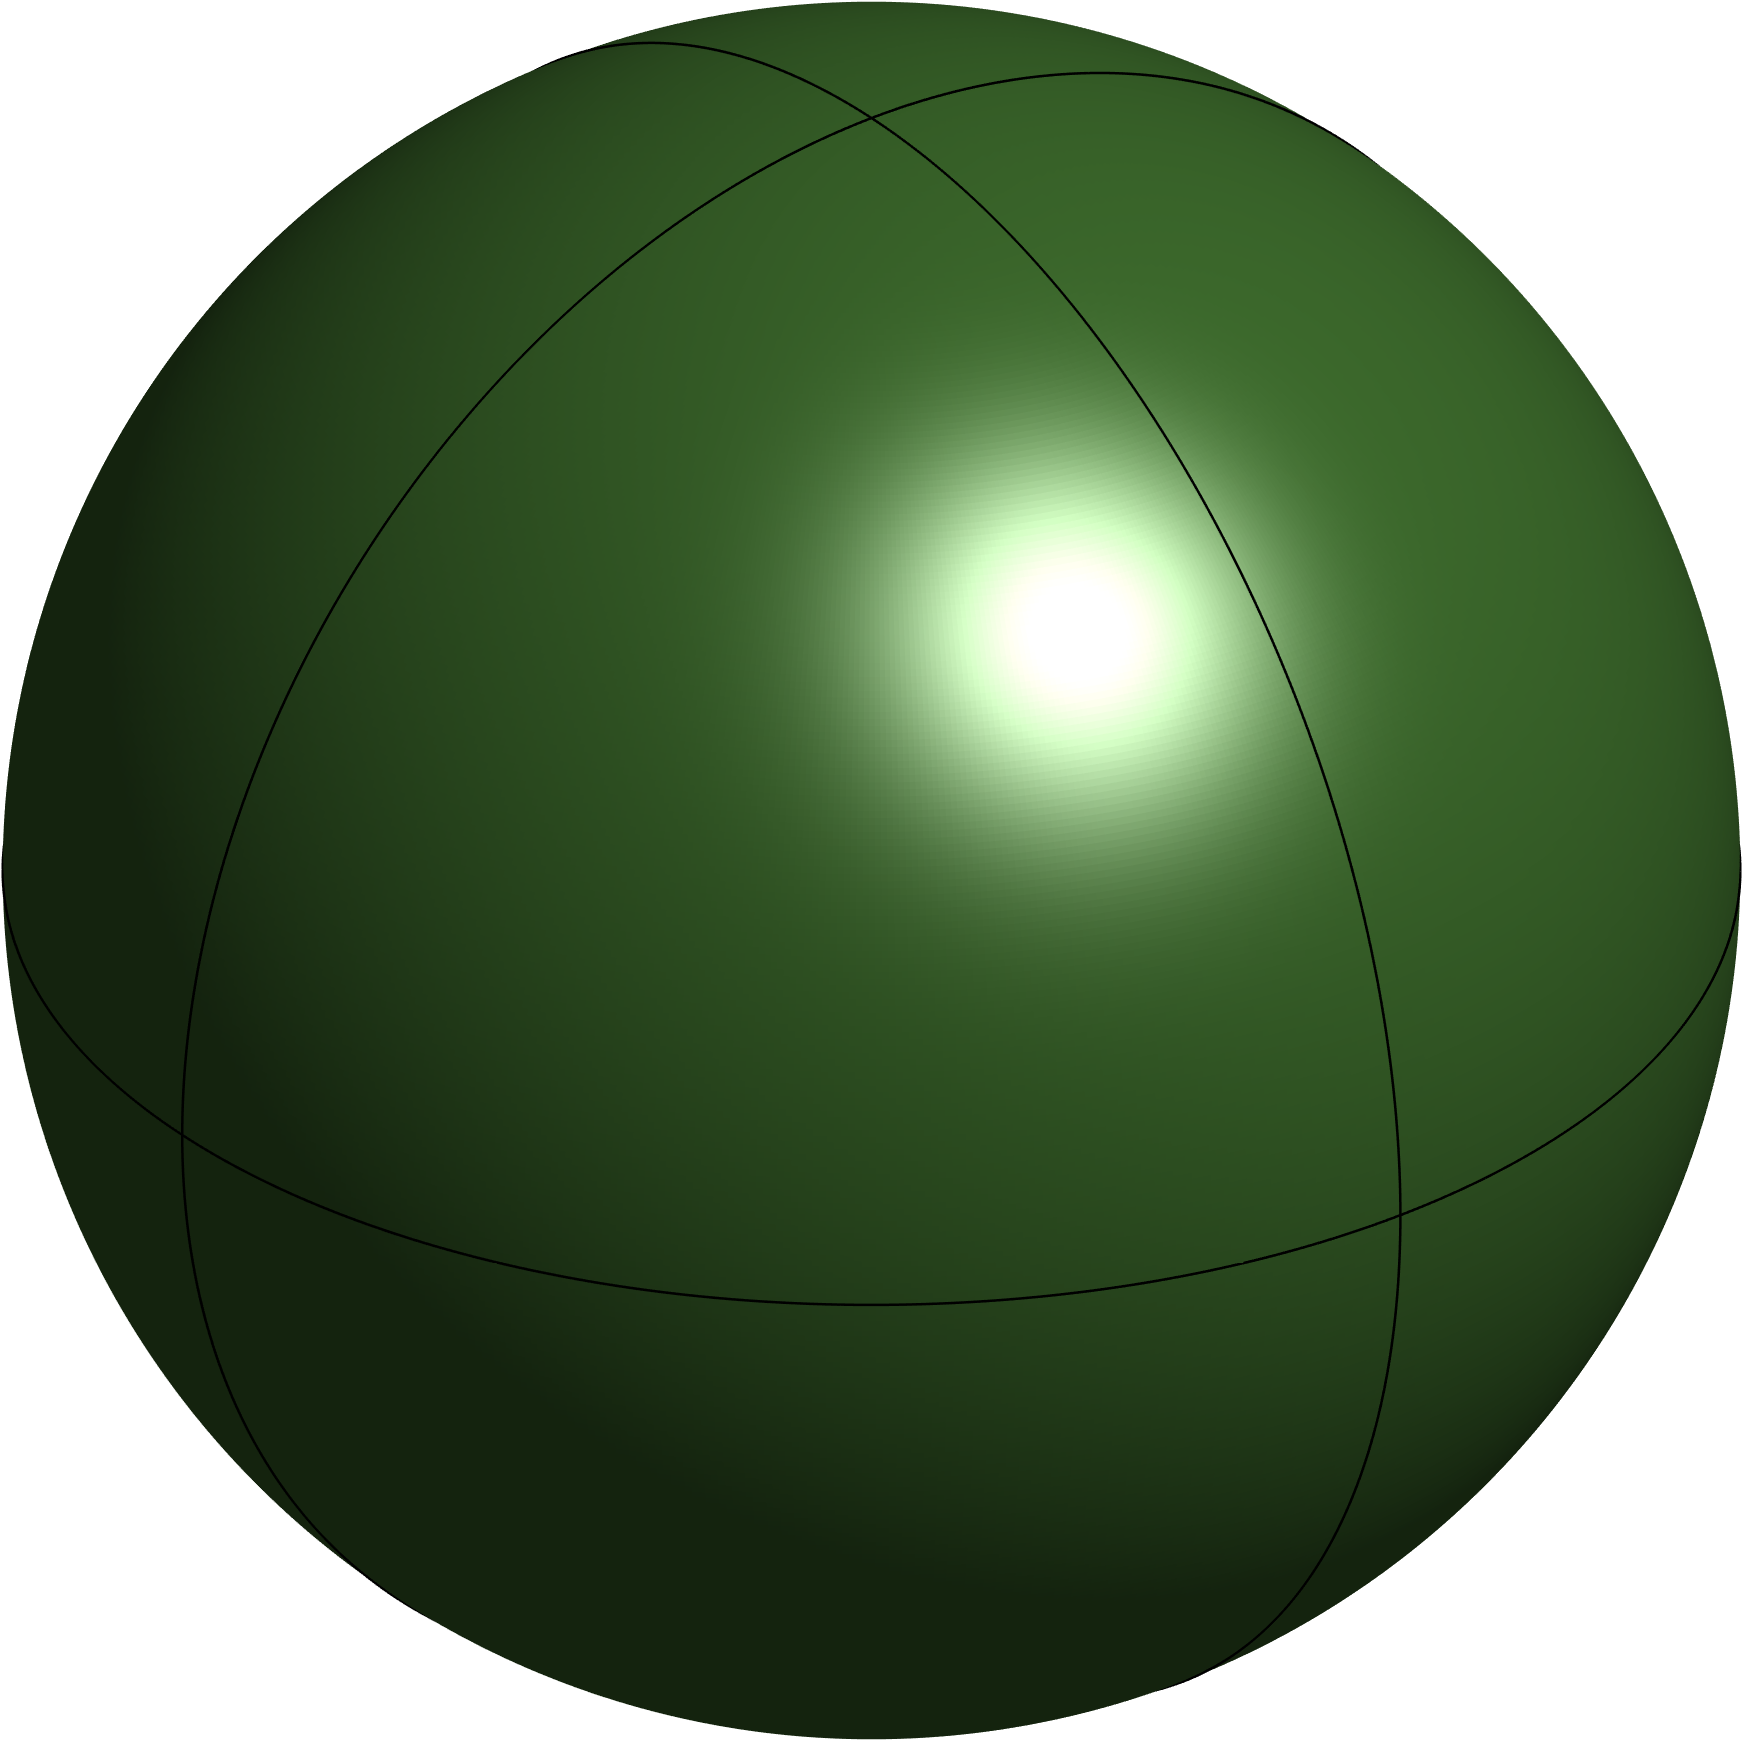
\includegraphics[width=0.8\textwidth]{sphericalShellMesh1_2_0}
		\caption{Mesh ${\cal M}_{1,\check{p},\check{k}}^{\textsc{iga}}$}
		\label{Fig2:SphericalShellMeshes1}
    \end{subfigure}
    ~
	\begin{subfigure}{0.3\textwidth}
		\centering
		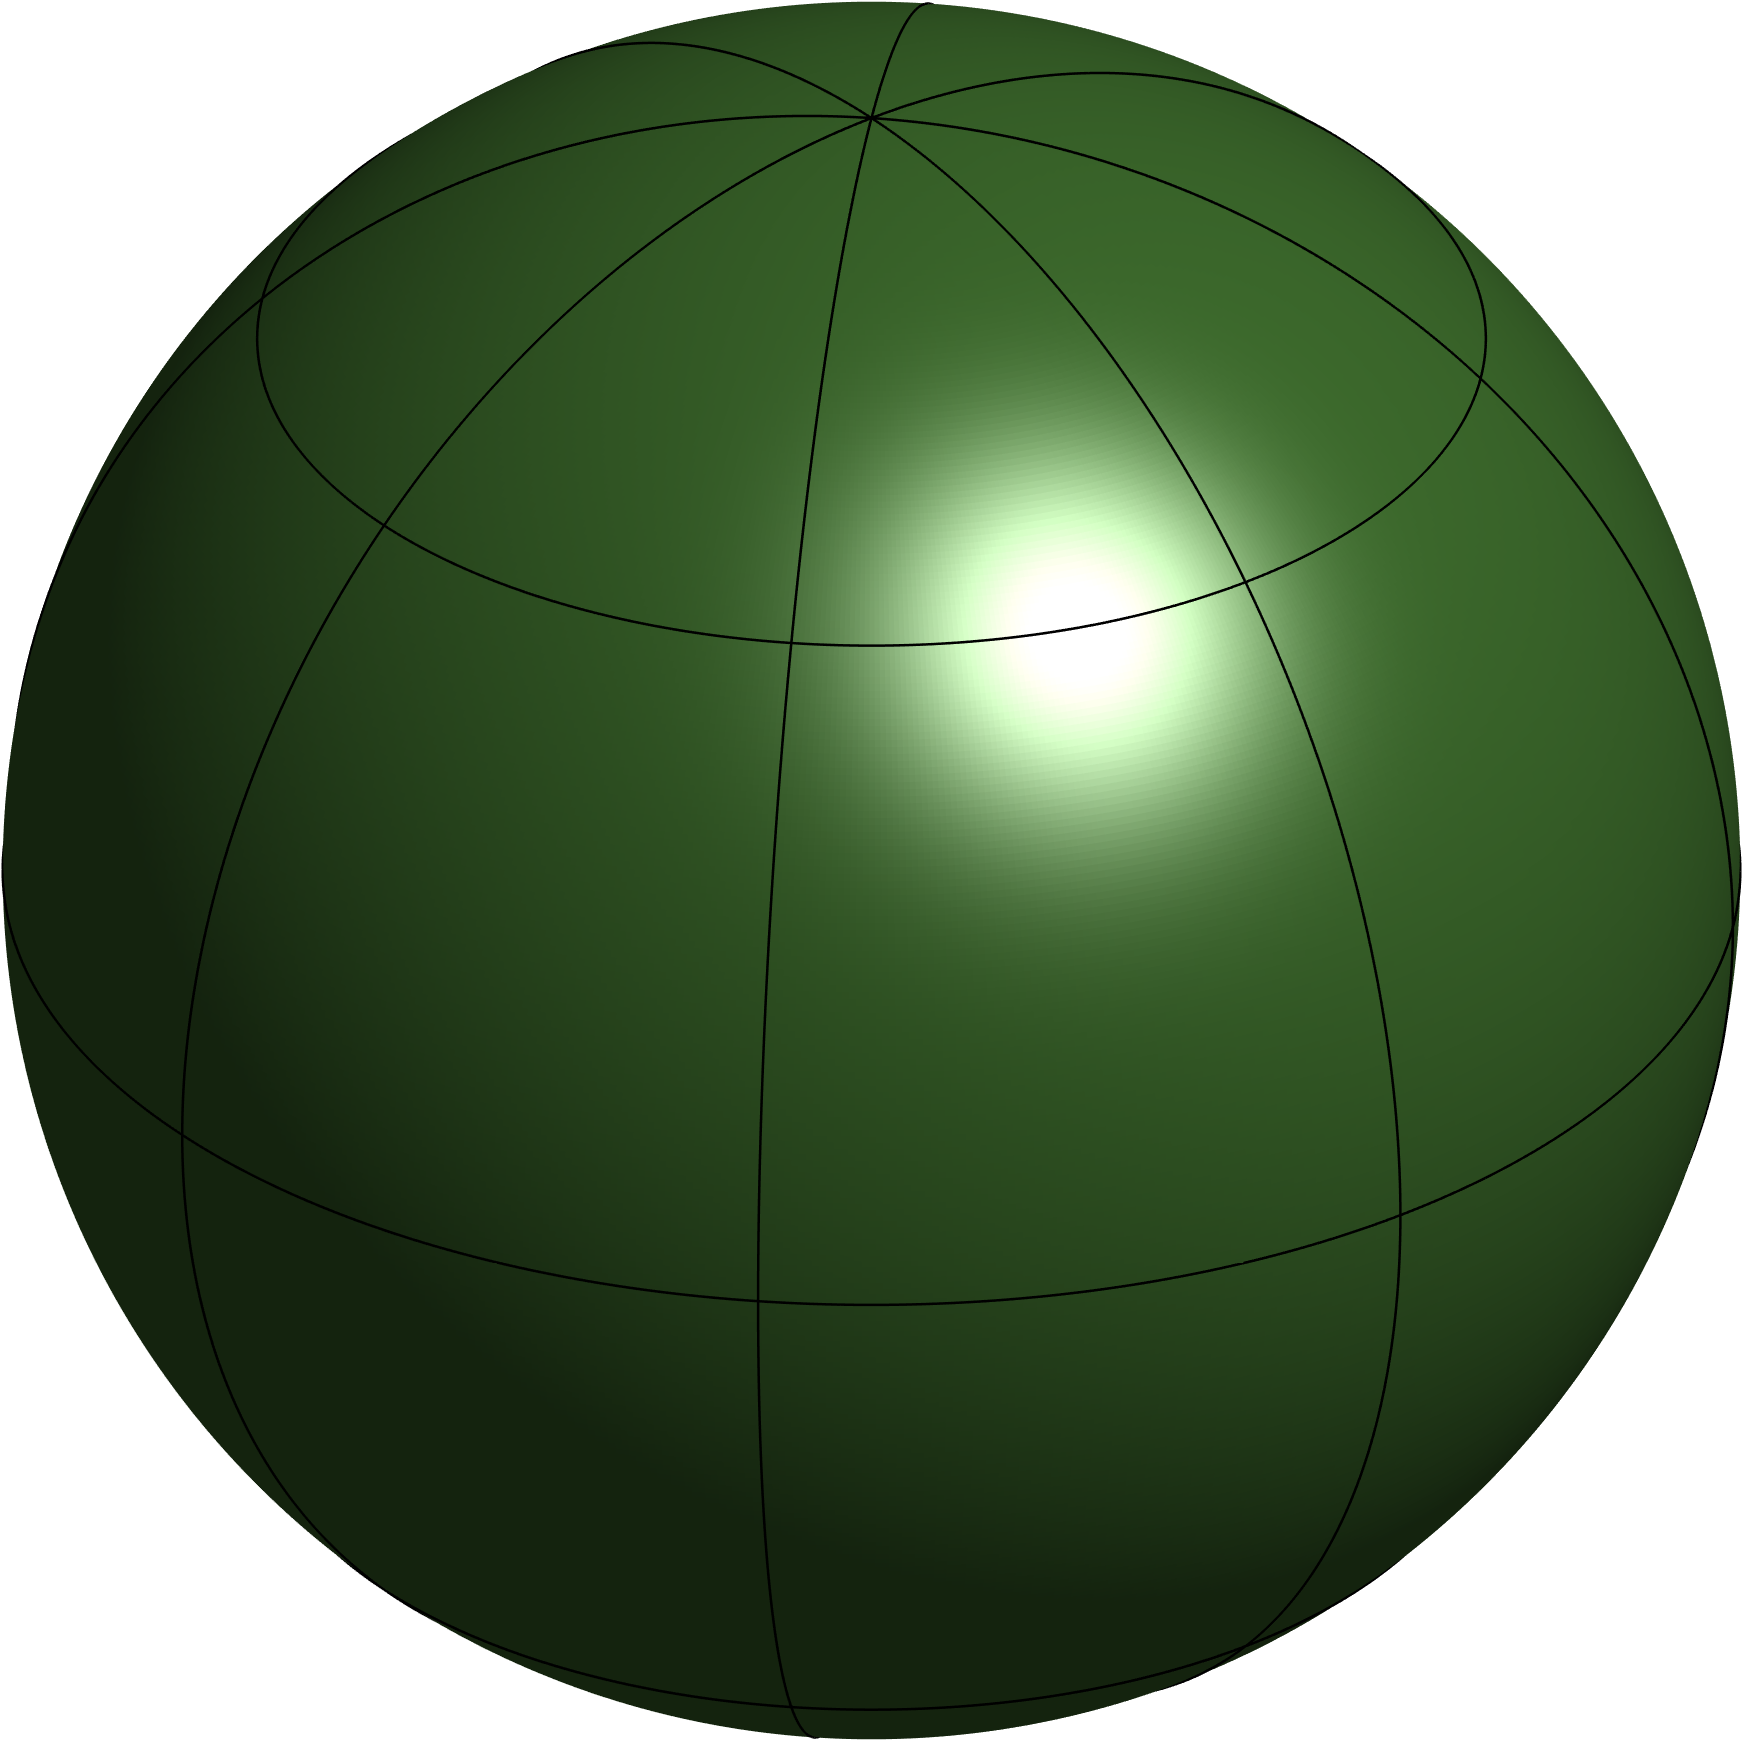
\includegraphics[width=0.8\textwidth]{sphericalShellMesh2_2_0}
		\caption{Mesh ${\cal M}_{2,\check{p},\check{k}}^{\textsc{iga}}$}
		\label{Fig2:SphericalShellMeshes2}
    \end{subfigure}
    ~
	\begin{subfigure}{0.3\textwidth}
		\centering
		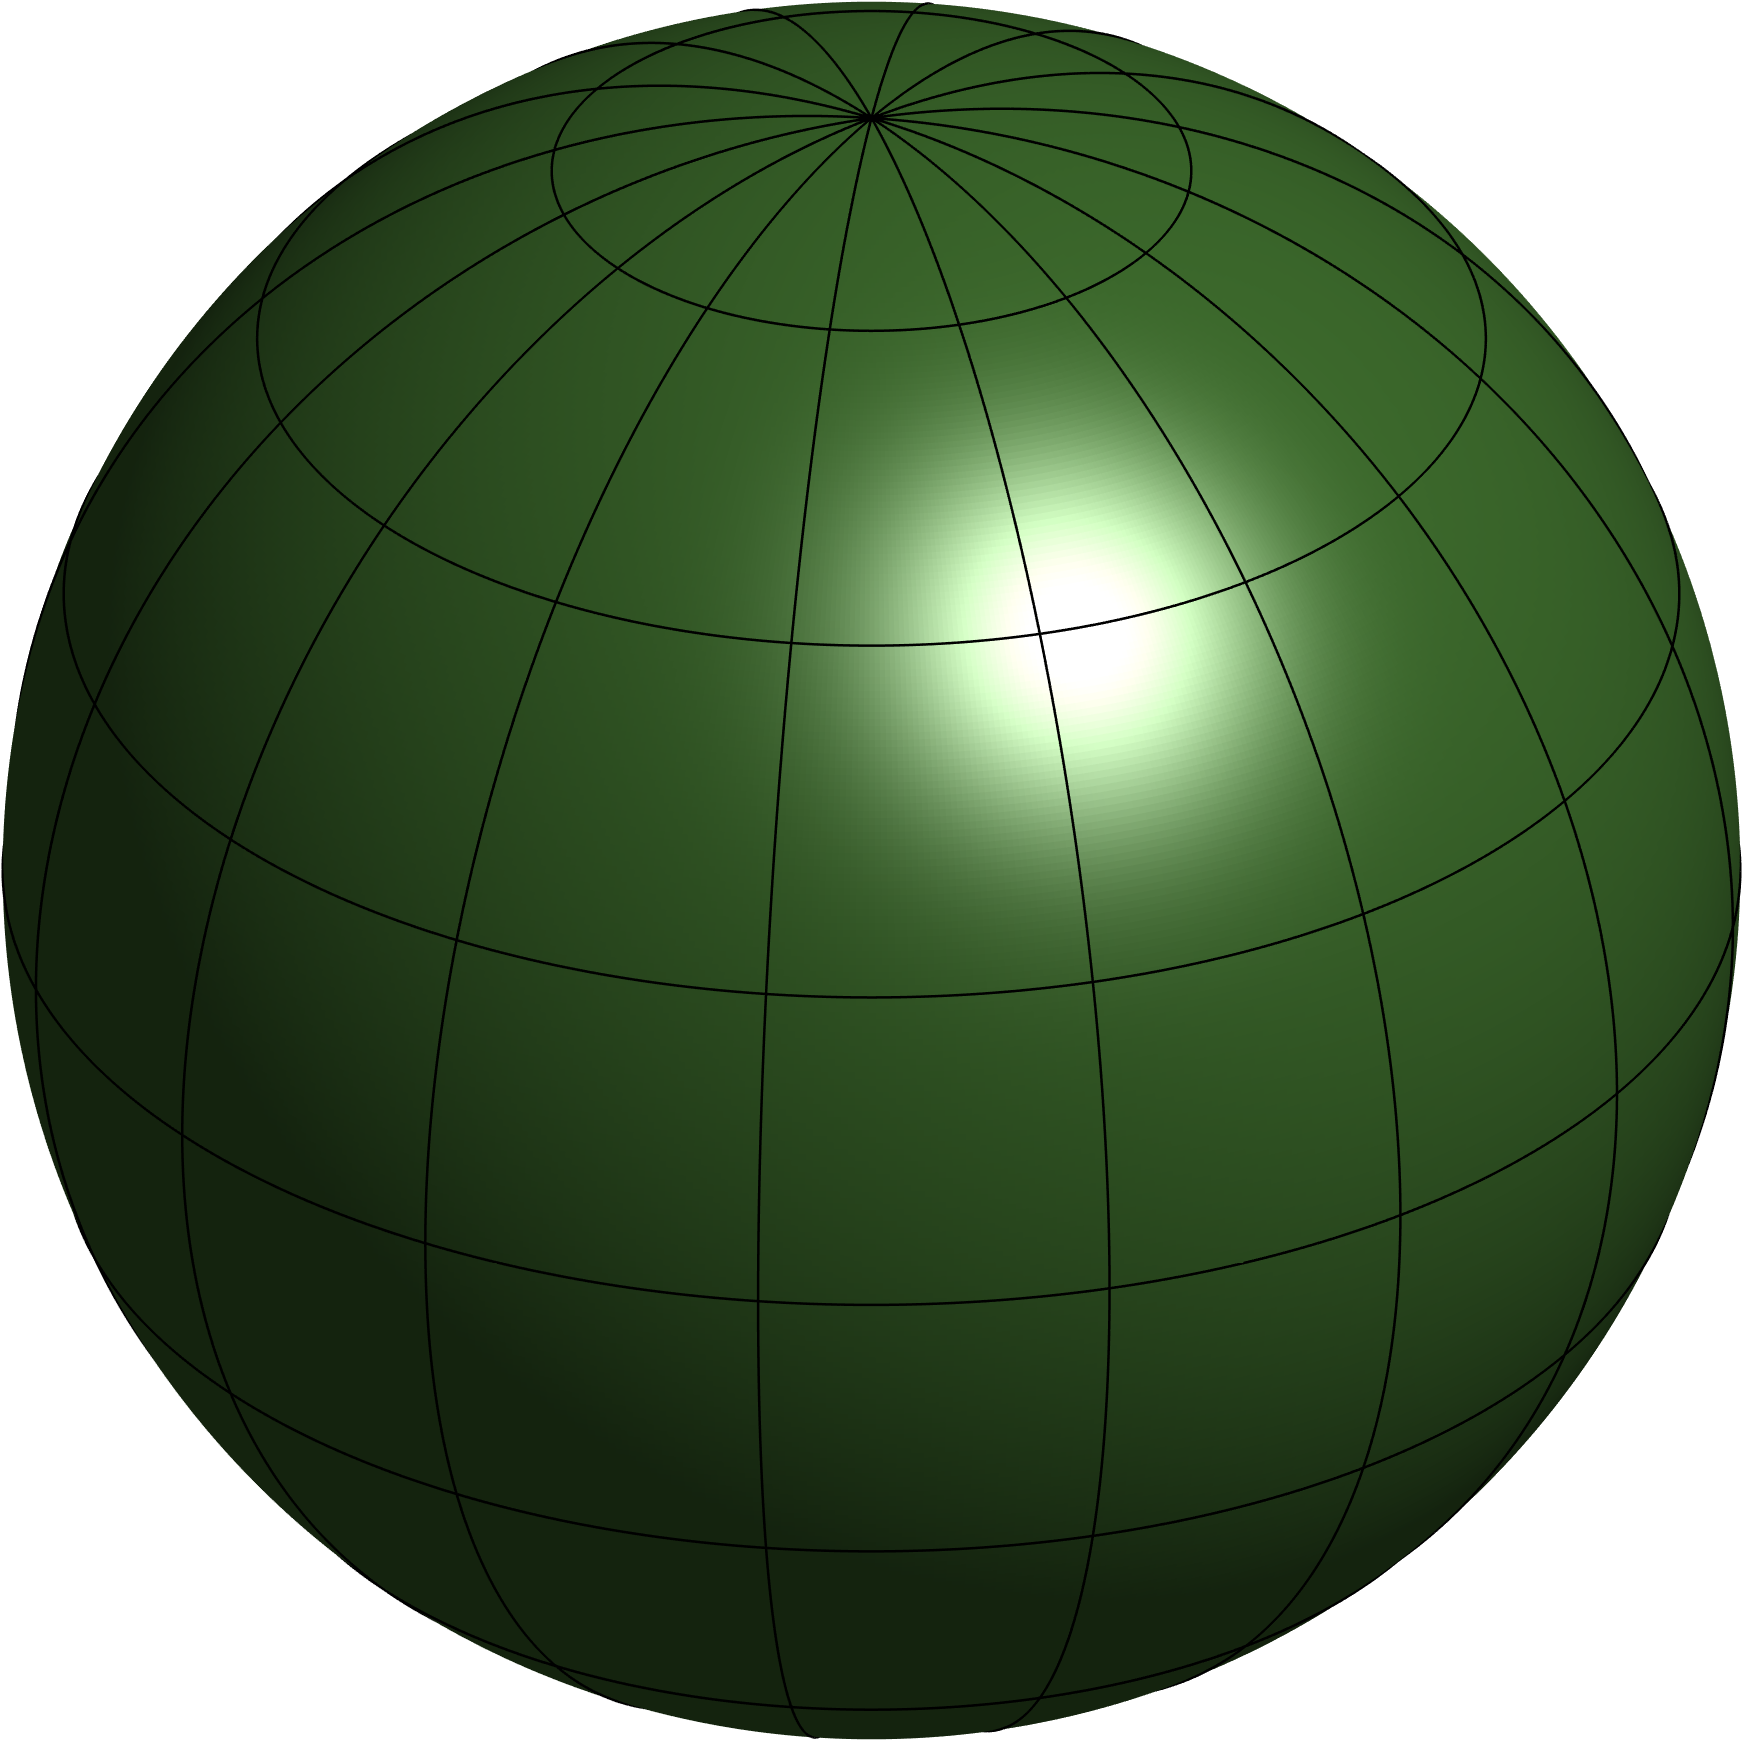
\includegraphics[width=0.8\textwidth]{sphericalShellMesh3_2_0}
		\caption{Mesh ${\cal M}_{3,\check{p},\check{k}}^{\textsc{iga}}$}
		\label{Fig2:SphericalShellMeshes3}
    \end{subfigure}
	\caption{\textbf{Numerical examples}: Illustration of the first three meshes, using two successive refinements from the coarse mesh ${\cal M}_{1,\check{p},\check{k}}^{\textsc{iga}}$.}
	\label{Fig2:SphericalShellMeshes}
\end{figure}

The meshes will be generated from a standard discretization of a sphere using NURBS as seen in \Cref{Fig2:SphericalShellMeshes}. We shall denote by ${\cal M}_{m,\check{p},\check{k}}^{\textsc{iga}}$, mesh number $m$ with polynomial order $\check{p}$ and continuity $\check{k}$ across element boundaries\footnote{Except for some possible $C^0$ lines in the initial CAD geometry.}. For the corresponding FEM meshes we denote by ${\cal M}_{m,\check{p},\mathrm{s}}^{\textsc{fem}}$ and ${\cal M}_{m,\check{p},\mathrm{i}}^{\textsc{fem}}$ the subparametric and isoparametric FEM meshes, respectively. The construction of NURBS meshes are illustrated in \Cref{Fig2:SphericalShellMeshes}. The initial mesh is depicted as mesh ${\cal M}_{1,\check{p},\check{k}}^{\textsc{iga}}$ in \Cref{Fig2:SphericalShellMeshes1} and is refined only in the angular directions for the first 3 refinements (that is, mesh ${\cal M}_{4,\check{p},\check{k}}^{\textsc{iga}}$ only have one element thickness in the radial direction). Mesh ${\cal M}_{m,\check{p},\check{k}}^{\textsc{iga}}$, $m=5,6,7$, have 2, 4 and 8 elements in its thickness, respectively. This is done to obtain low aspect ratios for the elements. All the meshes will then be nested and the refinements are done uniformly. We shall use the same polynomial order in all parameter directions; $\check{p}_\upxi=\check{p}_\upeta=\check{p}_\upzeta$. 

Unless otherwise stated, we shall use the BGU formulation and $N=4$ basis functions in the radial direction of the infinite elements.

\subsection{Simpson benchmark}
The configuration presented by Simpson et al.~\cite{Simpson2014aib} is considered: a rigid sphere of radius $R_0=\SI{0.5}{m}$ is impinged by an incident plane wave and the total pressure is measured at a distance $r=\SI{5}{m}$ from the origin. 

This is a low frequency problem with $k=\SI{2}{m^{-1}}$. It is emphasized that the trace of the NURBS discretization of the domain $\Omega_{\mathrm{a}}$ at the surface $\Gamma_0$ reduces to the exact same NURBS discretization used in~\cite{Simpson2014aib} to discretize the boundary $\Gamma_0$. 

From \Cref{Fig2:simpsonPlot} we observe that the IGA infinite element method (IGAIE) exploits the available degrees of freedom at $\Gamma_0$ more effectively than the IGA boundary element method (IGABEM) in~\cite{Simpson2014aib}\footnote{Due to low resolution of the plots in~\cite[Fig. 17]{Simpson2014aib}, the results were reproduced and sampled at 3601 points (rather than 30 points) using our own IGABEM implementation.}. 

By projecting the analytic solution onto this set of NURBS basis functions at $\Gamma_0$ (the best approximation in the $L_2$-norm by least squares projection, IGA best approximation, IGABA), it is revealed that even more accuracy can potentially be made. This is an inherent problem for Galerkin FEM when solving the Helmholtz equation and is related to the pollution effect \cite{Babuska1995agf}. All IEM formulations (PGU, PGC, BGU and BGC) gave approximately the same result in this case.
\begin{figure}
	\centering
	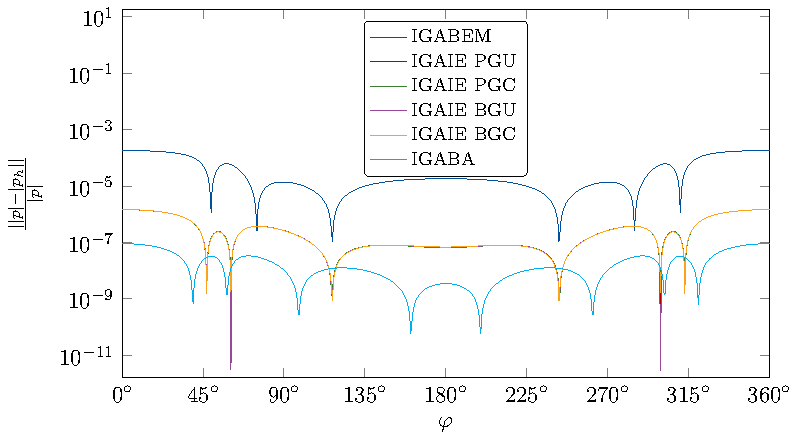
\includegraphics[width=\textwidth]{simpson}
	\caption{\textbf{Simpson benchmark}: The relative error in the modulus of the pressure is plotted on a circle (azimuth direction, $\varphi$) in the $xy$-plane at $r=\SI{5}{m}$. All simulations were computed on mesh ${\cal M}_{3,3,2}^{\textsc{iga}}$. The IGAIE formulations here produce roughly the same result.}
	\label{Fig2:simpsonPlot}
\end{figure}

\subsection{Ihlenburg benchmark}
Three benchmark solutions based on the model problem after Ihlenburg~\cite[p. 191]{Ihlenburg1998fea} with parameters given in \Cref{Tab2:IhlenburgParameters}, are investigated. 
\begin{table}
	\centering
	\caption{\textbf{Ihlenburg benchmark}: Parameters for the Ihlenburg benchmark problems.}
	\label{Tab2:IhlenburgParameters}
	\begin{tabular}{l l}
		\toprule
		Parameter & Description\\
		\midrule
		$P_{\mathrm{inc}}=\SI{1}{Pa}$ & Amplitude of incident wave\\
		$E = \SI{2.07e11}{Pa}$ & Young's modulus\\
		$\nu = 0.3$ & Poisson's ratio\\
		$\rho_{\mathrm{s}} = \SI{7669}{kg.m^{-3}}$ & Density of solid\\
		$\rho_{\mathrm{f}} = \SI{1000}{kg.m^{-3}}$ & Density of water\\
		$c_{\mathrm{f}} = \SI{1524}{m.s^{-1}}$ & Speed of sound in water\\
		$R_0=\SI{5.075}{m}$ & Outer radius\\
		$R_1=\SI{4.925}{m}$ & Inner radius\\
		\bottomrule
	\end{tabular}
\end{table}
The parameters for the fluid domains are the speed of sound in water $c_{\mathrm{f}}$ and the fluid density $\rho_{\mathrm{f}}$, and the parameters for the solid domain are the Young's modulus, $E$, the Poisson's ratio $\nu$ and the solid density $\rho_{\mathrm{s}}$. The first benchmark is a simple rigid scattering case (with sound-hard boundary conditions, SHBC) on a sphere with radius $R_0$. The second benchmark problem on a spherical shell has ASI conditions at the outer radius, $R_0$, and homogeneous Neumann condition at the inner radius, $R_1$ (sound-soft boundary conditions, SSBC). This case can be thought of as an approximation of a scattering problem on a spherical shell with an internal fluid with very low density. The third and final benchmark is a further extension with ASI conditions on both sides of the spherical shell (Neumann-Neumann conditions on both surfaces of the shell, NNBC). All of these benchmarks have analytic solutions~\cite{Venas2019e3s} (see \Cref{Fig2:ihlenburgTSexact,Fig2:ihlenburg3Dexact}), which enables computation of the error in the energy norm. As we use the same parameters in both fluids, we denote the common wave number in these fluids by $k=k_1=k_2$.
\begin{figure}
	\centering
	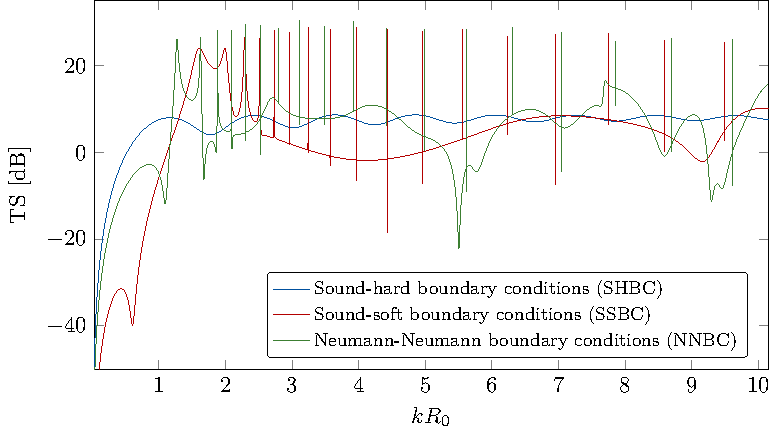
\includegraphics[width=\textwidth]{ihlenburg}
	\caption{\textbf{Ihlenburg benchmark}: Analytic solutions to the scattering problem on a spherical shell with parameters given in \Cref{Tab2:IhlenburgParameters}. The far field pattern of backscattered pressure is plotted against the wave number $k$. A single Neumann condition at the outer radius, $R_0$, corresponds to the rigid scattering case with $\vec{u}=\zerovec$ and $p_2=0$. ASI at $R_0$ and Neumann at $R_1$ models $p_2=0$. Note that Ihlenburg~\cite[p. 192]{Ihlenburg1998fea} plots the far field pattern in \Cref{Eq2:farfield} instead of the target strength, $\TS$, in \Cref{Eq2:TS}.}
	\label{Fig2:ihlenburgTSexact}
\end{figure}
\begin{figure}
	\centering
	\begin{subfigure}[t]{0.48\textwidth}
		\centering
		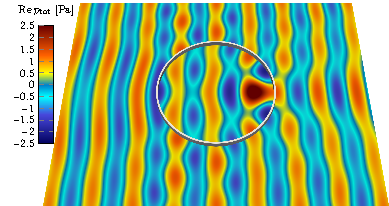
\includegraphics[width=\textwidth]{ihlenburg_nearField_real}
		\caption{Plot of the real part of the total pressure.}
	\end{subfigure}
	~
	\begin{subfigure}[t]{0.48\textwidth}
		\centering
		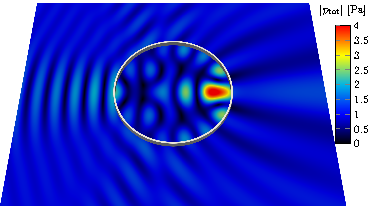
\includegraphics[width=\textwidth]{ihlenburg_nearField_abs}
		\caption{Plot of the modulus of the total pressure.}
	\end{subfigure}
	
	\caption{\textbf{Ihlenburg benchmark with NNBC}: The analytic solution with ASI at both $R_0$ and $R_1$ with $kR_0=10.15$ is plotted in the $xy$-plane. The solid domain is cut open for visualization purposes.}
	\label{Fig2:ihlenburg3Dexact}
\end{figure}
For each experiment, we use the same NURBS order everywhere. Denote by $\check{p}_\upxi = \check{p}_{\upxi,\mathrm{f}} = \check{p}_{\upxi,\mathrm{s}}$ the common NURBS order in the fluid and the solid in the $\xi$-direction. Similarly $\check{p}_\upeta = \check{p}_{\upeta,\mathrm{f}} = \check{p}_{\upeta,\mathrm{s}}$ and $\check{p}_\upzeta = \check{p}_{\upzeta,\mathrm{f}} = \check{p}_{\upzeta,\mathrm{s}}$. Moreover, we denote by $\check{p} = \check{p}_\upxi = \check{p}_\upeta = \check{p}_\upzeta$ the common polynomial orders in all domains.

In order to compare $C^0$ FEM and IGA on the scattering problem, we shall transform the NURBS mesh to a $C^0$ FEM mesh. We use the technique described in \Cref{Sec2:NURBStransformation} to get an isoparametric B-spline approximation of the geometry (isoparametric FEM). This parametrization will have $C^0$ continuity at element boundaries and correspondingly $G^0$ continuity of the geometry representation (i.e. with kinks). The geometric approximation error is of one order higher than the finite element approximation of the solution \cite{Strang1973aao}, so one could expect the $C^0$-IGA meshes (with $\check{k}=0$) to produce the same accuracy as the isoparametric FEM meshes of higher order ($\check{p}\geq 2$). It should be noted that the FEM analysis would then use the Bernstein basis instead of the classical Lagrange basis. However, both of these set of functions spans the same spaces, such that the results should be identical in the absence of round-off errors. 

In \Cref{Fig2:EnergyErrorPlotsDofs} we illustrate $h$-refinement through the error in the energy norm for the first benchmark example (rigid scattering).
\begin{figure}
	\centering
	\includegraphics[width=\textwidth]{L2normPlots_SHBC_dofs}
	\caption{\textbf{Ihlenburg benchmark with SHBC}: Convergence analysis on the rigid scattering case with $k=\SI{1}{m^{-1}}$ and mesh ${\cal M}_m$, $m=1,\dots,7$, using $N=6$. The relative energy error (\Cref{Eq2:energyNormFluids}) is plotted against the degrees of freedom.}
	\label{Fig2:EnergyErrorPlotsDofs}
	\par\bigskip
	\includegraphics[width=\textwidth]{L2normPlots_SHBC_nepw}
	\caption{\textbf{Ihlenburg benchmark with SHBC}: Convergence analysis on the rigid scattering case with $k=\SI{1}{m^{-1}}$ and mesh ${\cal M}_m$, $m=1,\dots,7$, using $N=6$. The relative energy error (\Cref{Eq2:energyNormFluids}) is plotted against the number of elements per wave.}
	\label{Fig2:EnergyErrorPlotsh}
\end{figure}
Predicted convergence rates are not obtained until the aspect ratio of the elements are reduced sufficiently (that is, from mesh ${\cal M}_4$ and onward). By comparing the results of mesh ${\cal M}_{m,2,\mathrm{i}}^{\textsc{fem}}$ and mesh ${\cal M}_{m,2,0}^{\textsc{iga}}$ it can be concluded that the geometry error of mesh ${\cal M}_{m,2,\mathrm{i}}^{\textsc{fem}}$ has almost no impact on the accuracy. However, when using maximum continuity, we get significantly better results. Expected convergence rates are visualized in \Cref{Fig2:EnergyErrorPlotsh} where we now plot the energy norm against $\lambda/h_{\mathrm{max}}$ (corresponding to the number of elements per wave) with $\lambda$ being the wavelength $\lambda=2\pi/k$. A key observation is that the number of elements per wave (needed to obtain a given accuracy) is greatly reduced with higher order IGA methods compared to the classical linear FEM (where 10 elements per wavelength is typically desired for engineering precision, \cite[p. 182]{Ihlenburg1998fea}). The result for the subparametric meshes ${\cal M}_{m,2,\mathrm{s}}^{\textsc{fem}}$ indicates that the convergence rate is reduced due to the reduced accuracy in the geometric representation. This is to be expected as shown in \cite[p. 202]{Strang1973aao}.

\begin{figure}
	\centering
	\begin{subfigure}{0.3\textwidth}
		\centering
		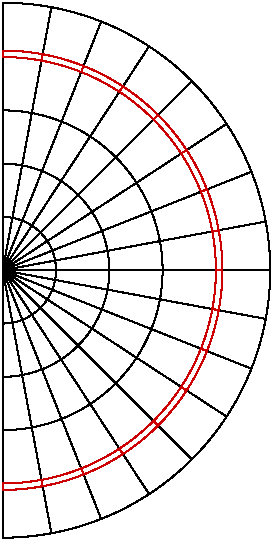
\includegraphics[width=0.6\textwidth]{NNBC_IGAmesh4}
		\caption{Mesh ${\cal M}_{4,\check{p},\check{k}}^{\textsc{iga}}$}
		\label{Fig2:SphericalShellMeshes1NNBC}
    \end{subfigure}
    ~
	\begin{subfigure}{0.3\textwidth}
		\centering
		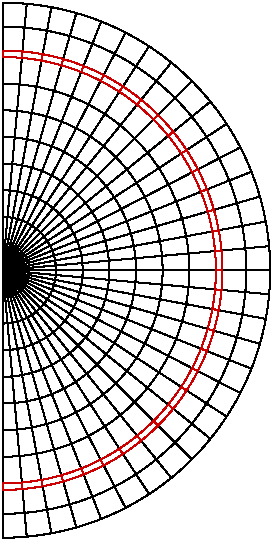
\includegraphics[width=0.6\textwidth]{NNBC_IGAmesh5}
		\caption{Mesh ${\cal M}_{5,\check{p},\check{k}}^{\textsc{iga}}$}
		\label{Fig2:SphericalShellMeshes2NNBC}
    \end{subfigure}
    ~
	\begin{subfigure}{0.3\textwidth}
		\centering
		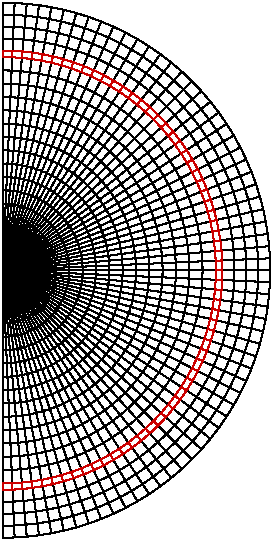
\includegraphics[width=0.6\textwidth]{NNBC_FEMlinear6}
		\caption{Mesh ${\cal M}_{6,1,\mathrm{i}}^{\textsc{fem}}$}
		\label{Fig2:SphericalShellMeshes3NNBC}
    \end{subfigure}
	\caption{\textbf{Ihlenburg benchmark with NNBC}: Illustration of some meshes for the full ASI problem in the $xz$-plane ($x>0$), where the mesh lines for the solid domain is colored red. The full mesh is obtained by rotation around the $z$-axis. Mesh ${\cal M}_{5,2,\mathrm{i}}^{\textsc{fem}}$ is visually indistinguishable from ${\cal M}_{5,\check{p},\check{k}}^{\textsc{iga}}$.}
	\label{Fig2:SphericalShellMeshesNNBC}
\end{figure}
Approaching the ASI problems, we illustrate some meshes in \Cref{Fig2:SphericalShellMeshesNNBC} for the full ASI problem. The corresponding meshes for the SSBC problem (with $p_2=0$) are obtained by removing the mesh inside the solid domain. In \Cref{Fig2:TSPlotSHBC,Fig2:errorPlotSHBC,Fig2:TSPlotSSBC,Fig2:errorPlotSSBC,Fig2:TSPlotNNBC,Fig2:errorPlotNNBC} the target strength, $\TS$, and the error in the energy norm is plotted against the scaled wave number, $kR_0$, in all of the three Ihlenburg benchmarks. As each frequency sweep is computed with a different number of degrees of freedom, one should draw the conclusions based on comparing both the accuracy of the results and the related computational costs.

Some data from simulations at $k=\SI{1}{m^{-1}}$ are reported in \Cref{Tab2:dataRigidScattering} (simulation run with 12 processors of the type Intel(R) Xeon(R) CPU E5-4650 2.70GHz). It should be noted that all simulations were done using the same code, such that the computational time for the FEM simulations can be optimized. However, this is actually the case for the IGA code as well since the implementation does not utilize optimized quadrature rules. The integration is done with $(\check{p}+1)^3$ quadrature points per element when building the system. For higher order splines spaces this is significantly more quadrature point than what is needed for exact integration (on meshes with affine geometry mapping\footnote{Using the same quadrature scheme on truly isoparametric elements will according to \cite[p. 256]{Ciarlet1991bee} give a numerical integration error of the same order as the finite element discretization error. Thus, the argument for optimal quadrature scheme also holds for isoparametric elements as well.}). In \cite{Hughes2010eqf,Johannessen2017oqf}, it is shown that the optimal number of quadrature points is half the number of degrees of freedom of the splines space under consideration. That is, the number of quadrature points in the IGA 3D tensor product meshes can be reduced by a factor up to $2^3(\check{p}+1)^3$ for meshes with maximal continuity. Thus, the efficiency of the IGA simulation may be improved significantly.

A particular interesting observation is that IGA obtains roughly the same accuracy as FEM when the same number of elements is used, even though this corresponds to far less degrees of freedom for the IGA simulation. Moreover, even better result can be obtained with less degrees of freedom if the polynomial degree is increased in the IGA simulations. This, however, only occurs when the mesh resolves the number of waves per element. When the mesh is sufficiently resolved, one order of magnitude improvement in the accuracy is obtained by increasing the polynomial degree. Since another magnitude of accuracy is obtained by using higher order elements in FEM/IGA, the IGA offers several orders of magnitude better accuracy than classical linear FEM. 

The peaks in the frequency sweeps represent eigenmodes. The quality of the numerical approximation of the corresponding frequencies is reduced for higher frequencies, resulting in fictitious modes. This typically does not pose that much of a problem as the bandwidth of these eigenmodes becomes very small, with a corresponding reduction in the energy they represent. Note that mesh ${\cal M}_{4,3,2}^{\textsc{iga}}$ performs particularly poorly on the partial ASI problem due to a fictitious mode at $k=\SI{1}{m^{-1}}$ for this mesh. The improvement offered by IGA concerning the accuracy in the eigenmodes is investigated in~\cite{Venas2015iao}. 

It should be noted that the meshes used throughout this work are not optimal. This is in particular the case for the full ASI problem where the density of elements becomes large at the origin. These meshes were used as they naturally arise from tensor product NURBS meshes of spherical shells and spheres. One could thus obtain increased performance for the FEM solutions using standard meshing of the domain. However, locally refined meshes can also be obtained with the IGA method, for example using LR B-splines \cite{Johannessen2014iau}.

\begin{table}
	\centering
	\caption{\textbf{Ihlenburg benchmark}: Data for some simulations on the rigid scattering problem with $k=\SI{1}{m^{-1}}$. The errors are given in the energy norm (\Cref{Eq2:energyNorm}). For each simulation, the mesh number, the polynomial order, $\check{p}$, the number of mesh elements $n_{\mathrm{el}}$ (not including the infinite elements) and the number of degrees of freedom $n_{\mathrm{dof}}$, is reported. The elapsed times for building the system $t_{\mathrm{sys}}$ and for solving the system $t_{\mathrm{sol}}$ (using LU-factorization) are also included (times in seconds). Finally, the relative error in the energy norm is given in percentage.}
	\label{Tab2:dataRigidScattering}
	\begin{subtable}[t]{\linewidth}
		\caption{Sound-hard boundary conditions (SHBC).}
		\label{Tab2:dataRigidScatteringSHBC}
		\centering
		\bgroup
		\def\arraystretch{1.1}%
		\begin{tabular}{l S[table-format = 6.0] S[table-format = 5.0] S[table-format = 2.1,round-mode=places,round-precision=1] S[table-format = 2.1,round-mode=places,round-precision=1] S[table-format = 1.2]}
			\hline
			 		   & {$n_{\mathrm{el}}$} & {$n_{\mathrm{dof}}$} &{$t_{\mathrm{sys}}$ [s]}	& {$t_{\mathrm{sol}}$ [s]} 		& {Relative energy error [\%]} \\
			\hline
			Mesh ${\cal M}_{6,1,\mathrm{i}}^{\textsc{fem}}$		& 32768	& 56462	& 7.70	& 26.50	& 5.04	\cr
Mesh ${\cal M}_{5,2,\mathrm{i}}^{\textsc{fem}}$		& 4096	& 56462	& 5.07	& 20.48	& 0.62	\cr
Mesh ${\cal M}_{5,2,1}^{\textsc{iga}}$				& 4096	& 13476	& 4.79	& 4.32	& 0.64	\cr
Mesh ${\cal M}_{4,3,2}^{\textsc{iga}}$				& 512	& 4572	& 3.06	& 1.64	& 0.38	\cr
Mesh ${\cal M}_{5,3,2}^{\textsc{iga}}$				& 4096	& 17654	& 14.75	& 8.30	& 0.05	\cr

			\hline
		\end{tabular}
		\egroup
	\end{subtable}
	\par\bigskip
	\begin{subtable}[t]{\linewidth}
		\caption{Sound-soft boundary conditions (SSBC).}
		\label{Tab2:dataRigidScatteringSSBC}
		\centering
		\bgroup
		\def\arraystretch{1.1}%
		\begin{tabular}{l S[table-format = 6.0] S[table-format = 6.0] S[table-format = 2.1,round-mode=places,round-precision=1] S[table-format = 3.1,round-mode=places,round-precision=1] S[table-format = 2.2]}
			\hline
			 		   & {$n_{\mathrm{el}}$} & {$n_{\mathrm{dof}}$} &{$t_{\mathrm{sys}}$ [s]}	& {$t_{\mathrm{sol}}$ [s]} 		& {Relative energy error [\%]} \\
			\hline
			Mesh ${\cal M}_{6,1,\mathrm{i}}^{\textsc{fem}}$		& 40960	& 104858	& 13.66	& 75.28	& 7.66	\cr
Mesh ${\cal M}_{5,2,\mathrm{i}}^{\textsc{fem}}$		& 6144	& 129056	& 15.85	& 106.07	& 1.35	\cr
Mesh ${\cal M}_{5,2,1}^{\textsc{iga}}$				& 6144	& 33690	& 13.35	& 34.68	& 0.99	\cr
Mesh ${\cal M}_{4,3,2}^{\textsc{iga}}$				& 1024	& 13716	& 11.83	& 9.04	& 41.30	\cr
Mesh ${\cal M}_{5,3,2}^{\textsc{iga}}$				& 6144	& 47918	& 52.03	& 69.94	& 0.09	\cr

		    \hline
		\end{tabular}
		\egroup
	\end{subtable}	
	\par\bigskip
	\begin{subtable}[t]{\linewidth}
		\caption{Neumann-Neumann boundary conditions (NNBC).}
		\label{Tab2:dataRigidScatteringNNBC}
		\centering
		\bgroup
		\def\arraystretch{1.1}%
		\begin{tabular}{l S[table-format = 6.0] S[table-format = 6.0] S[table-format = 2.1,round-mode=places,round-precision=1] S[table-format = 3.1,round-mode=places,round-precision=1] S[table-format = 1.2]}
			\hline
			 		  & {$n_{\mathrm{el}}$} & {$n_{\mathrm{dof}}$} &{$t_{\mathrm{sys}}$ [s]}	& {$t_{\mathrm{sol}}$ [s]} 		& {Relative energy error [\%]} \\
			\hline
			Mesh ${\cal M}_{6,1,\mathrm{i}}^{\textsc{fem}}$		& 172032	& 233915	& 27.80	& 429.52	& 6.55	\cr
Mesh ${\cal M}_{5,2,\mathrm{i}}^{\textsc{fem}}$		& 22528	& 258113	& 31.05	& 462.66	& 0.53	\cr
Mesh ${\cal M}_{5,2,1}^{\textsc{iga}}$				& 22528	& 53905	& 22.46	& 64.91	& 0.71	\cr
Mesh ${\cal M}_{4,3,2}^{\textsc{iga}}$				& 3072	& 18289	& 17.10	& 17.28	& 1.47	\cr
Mesh ${\cal M}_{5,3,2}^{\textsc{iga}}$				& 22528	& 73139	& 93.22	& 145.74	& 0.05	\cr

		    \hline
		\end{tabular}
		\egroup
	\end{subtable}	
\end{table}

\begin{figure}
	\centering
	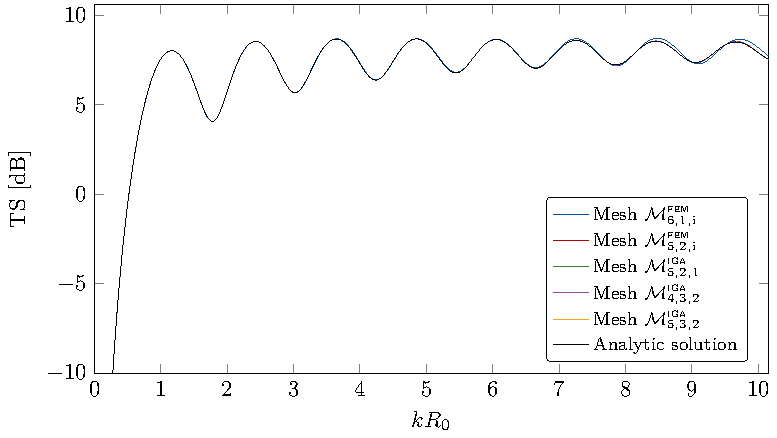
\includegraphics[width=\textwidth]{ihlenburg_farField_TSPlotSHBC}
	\caption{\textbf{Ihlenburg benchmark with SHBC}: The target strength (TS) in \Cref{Eq2:TS} is plotted against $kR_0$.}
	\label{Fig2:TSPlotSHBC}
	\par\bigskip
	\par\bigskip
	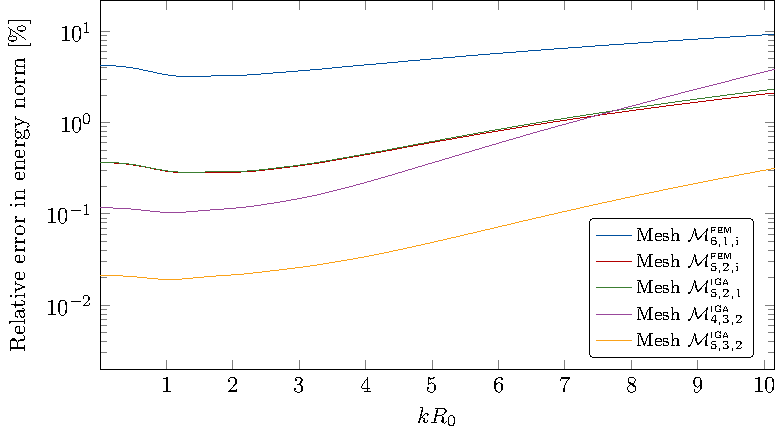
\includegraphics[width=\textwidth]{ihlenburg_farField_errorPlotSHBC}
	\caption{\textbf{Ihlenburg benchmark with SHBC}: The relative energy norm (\Cref{Eq2:energyNorm}) is plotted against $kR_0$.}
	\label{Fig2:errorPlotSHBC}
\end{figure}
\begin{figure}
	\centering
	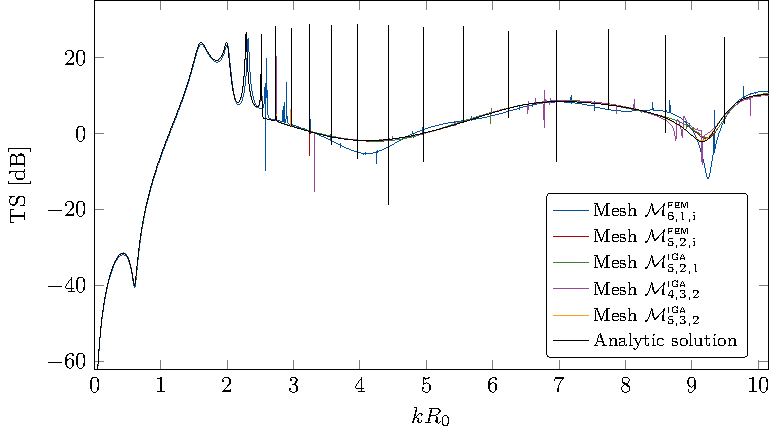
\includegraphics[width=\textwidth]{ihlenburg_farField_TSPlotSSBC}
	\caption{\textbf{Ihlenburg benchmark with SSBC}: ASI problem with the internal pressure modeled to be $p_2=0$. The target strength (TS) in \Cref{Eq2:TS} is plotted against $kR_0$.}
	\label{Fig2:TSPlotSSBC}
	\par\bigskip
	\par\bigskip
	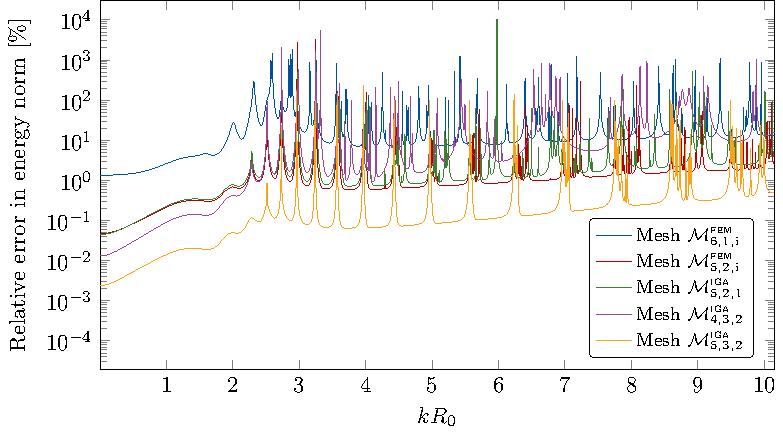
\includegraphics[width=\textwidth]{ihlenburg_farField_errorPlotSSBC}
	\caption{\textbf{Ihlenburg benchmark with SSBC}: ASI problem with the internal pressure modeled to be $p_2=0$. The relative energy norm (\Cref{Eq2:energyNorm}) is plotted against $kR_0$.}
	\label{Fig2:errorPlotSSBC}
\end{figure}
\begin{figure}
	\centering
	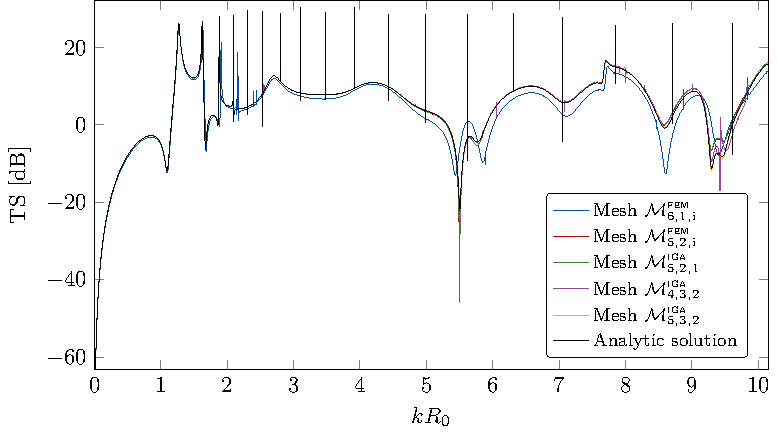
\includegraphics[width=\textwidth]{ihlenburg_farField_TSPlotNNBC}
	\caption{\textbf{Ihlenburg benchmark with NNBC}: The target strength (TS) in \Cref{Eq2:TS} is plotted against $kR_0$.}
	\label{Fig2:TSPlotNNBC}
	\par\bigskip
	\par\bigskip
	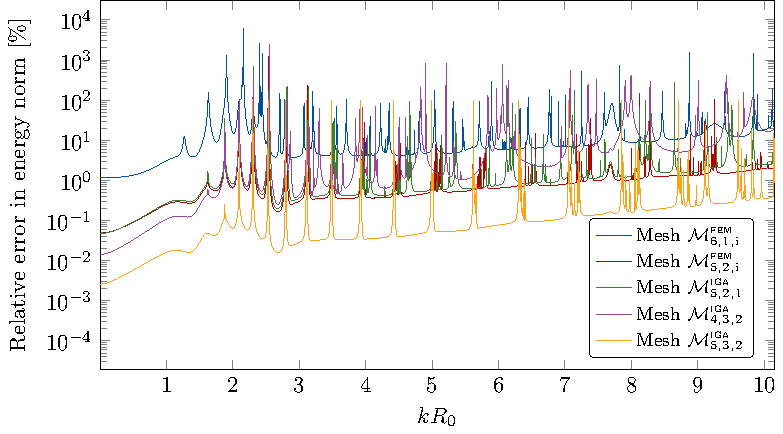
\includegraphics[width=\textwidth]{ihlenburg_farField_errorPlotNNBC}
	\caption{\textbf{Ihlenburg benchmark with NNBC}: The relative energy norm (\Cref{Eq2:energyNorm}) is plotted against $kR_0$.}
	\label{Fig2:errorPlotNNBC}
\end{figure}
In \Cref{Fig2:energyErrorPlot} we visualize the distribution of the error of the full ASI problem. The error is observed to be largest at element boundaries where the continuity is reduced. Since second order basis functions are used and the error in the velocity/stress dominates the error in the pressure/displacement, the results are in agreement with what was observed in \cite{Kumar2017spr}, i.e., that the error in the derivative of the primary solution is largest at the element boundaries.
\begin{figure}
	\centering
	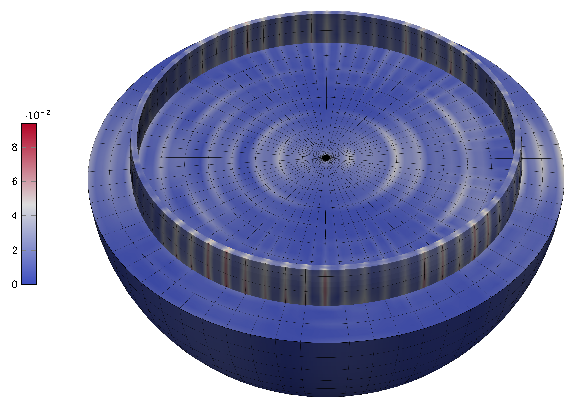
\includegraphics[width=0.7\textwidth]{energyErrorPlot}
	\caption{\textbf{Ihlenburg benchmark with NNBC}: Simulation of the full ASI problem on mesh ${\cal M}_{5,2,1}^{\textsc{iga}}$. Pointwise evaluation of the square root of the integrand of the volume integrals in the energy norm $\energyNorm{U-U_h}{\Omega}$ in \Cref{Eq2:energyNorm} with $k=\SI{2}{m^{-1}}$ (error in the infinite elements in $\Omega_{\mathrm{a}}^+$ is not shown) is here visualized, where $U$ is the set of analytic solutions in both fluid domains and the solid domain, and $U_h$ is the corresponding numerical solution. The values are scaled by the square root of the maximum of the corresponding integrand values of $\energyNorm{U}{\Omega}$. Both fluid domains are cut open at the $xy$-plane (at $z=0$), and the solid domain is cut open at $z=\SI{1.1}{m}$.}
	\label{Fig2:energyErrorPlot}
\end{figure}

\subsection{Radial pulsation from a mock shell}
\label{Subsec2:mockShell}
By construction of the fundamental solution of the Helmholtz equation ($\Phi_k(\vec{x},\vec{y})$ in \Cref{Eq2:FreeSpaceGrensFunction}), the function $p(\vec{x}) = \Phi_k(\vec{x},\vec{y})$ is a solution to \Cref{Eq2:HelmholtzEqn,Eq2:HelmholtzEqnNeumannCond,Eq2:sommerfeldCond} whenever $\vec{y}\in\R^3\setminus\overline{\Omega^+}$ and for the Neumann boundary condition $g(\vec{x})=\partial_n\Phi_k(\vec{x},\vec{y})$ on $\Gamma_0$.  Hence, we have an exact reference solution for the exterior Helmholtz problem for arbitrary geometries $\Gamma_0$ which encloses the point $\vec{y}$. It is emphasized that this solution is non-physical for non-spherical geometries $\Gamma_0$. General solutions may be constructed by separation of variables (cf.~\cite[p. 26]{Ihlenburg1998fea})
\begin{equation}
	p(\vec{x}) = \sum_{n=0}^\infty\sum_{m=-n}^n C_{nm} \hankel_n^{(1)}(kR) \legendre_n^{|m|}(\cos\vartheta)\euler^{\imag m\varphi} 
\end{equation}
with
\begin{equation*}
	R = |\vec{x}-\vec{y}|,\quad \vartheta=\arccos\left(\frac{x_3-y_3}{R}\right),\quad\varphi = \operatorname{atan2}(x_2-y_2,x_1-y_1)
\end{equation*}
where $\hankel_n^{(1)}$ is the $n^{\mathrm{th}}$ spherical Hankel function of first kind and $\legendre_n^m$ are the associated Legendre functions. In fact, the solution $p(\vec{x}) = \Phi_k(\vec{x},\vec{y})$ is a special case of this general form with 
\begin{equation}
	C_{nm} = \begin{cases}
		\frac{\imag k}{4\PI} & n = 0,\,\,m=0\\
		0 & \text{otherwise}.
		\end{cases}
\end{equation}
The complexity of this problem setup does not scale with the complexity of the model as it is independent of $\Gamma_0$. However, it preserves two important properties of acoustic scattering, namely the radial decay and the oscillatory nature. Thus, this problem setup represents a general way of constructing manufactured solutions, that can be utilized to verify the correctness of the implemented code for solving the Helmholtz equation. A special case of this general setup is the pulsating sphere example in~\cite{Simpson2014aib}.

From the first limit of \Cref{Eq2:Phi_k_limits1,Eq2:Phi_k_limits2}, the far field is given by $p_0(\hat{\vec{x}})=\frac{1}{4\PI}\euler^{-\imag k \hat{\vec{x}}\cdot\vec{y}}$. Thus, the target strength is a constant, $\TS=-20\log_{10}(4\PI)\approx -21.984$ (where we define $P_{\mathrm{inc}}=\SI{1}{Pa}$ in \Cref{Eq2:TS} for this problem). 

Consider the case $\vec{y}=\frac{R_0}{4}(1,1,1)$ and the boundary $\Gamma_0$ given by a \textit{mock shell} composed of a cylinder with hemispherical endcaps (with axis of symmetry along the $x$-axis such that the center of the spherical endcaps are located at $x = 0$ and $x = -L$). The cylinder has radius $R_0=\SI{1}{m}$ and length $L=\frac{\PI}{2}R_0$. The analytic solution is given by
\begin{equation}
	p(\vec{x}) = \frac{\euler^{\imag kR}}{4\PI R},\quad R=|\vec{x}-\vec{y}|
\end{equation}
and the Neumann condition is then
\begin{equation}
	g(\vec{x}) = \frac{\euler^{\imag kR}}{4\PI R^3}(\imag kR -1) (\vec{x}-\vec{y})\cdot\vec{n}(\vec{x}).
\end{equation}

This example is used to illustrate the differences of the infinite element formulations using the prolate ellipsoidal elements after Burnett~\cite{Burnett1994atd}. The mesh construction is illustrated in \Cref{Fig2:MS_meshes}, and an illustration of the solution is presented in \Cref{Fig2:MS_visualization}.
\begin{figure}
	\centering    
	\begin{subfigure}{0.49\textwidth}
		\centering
		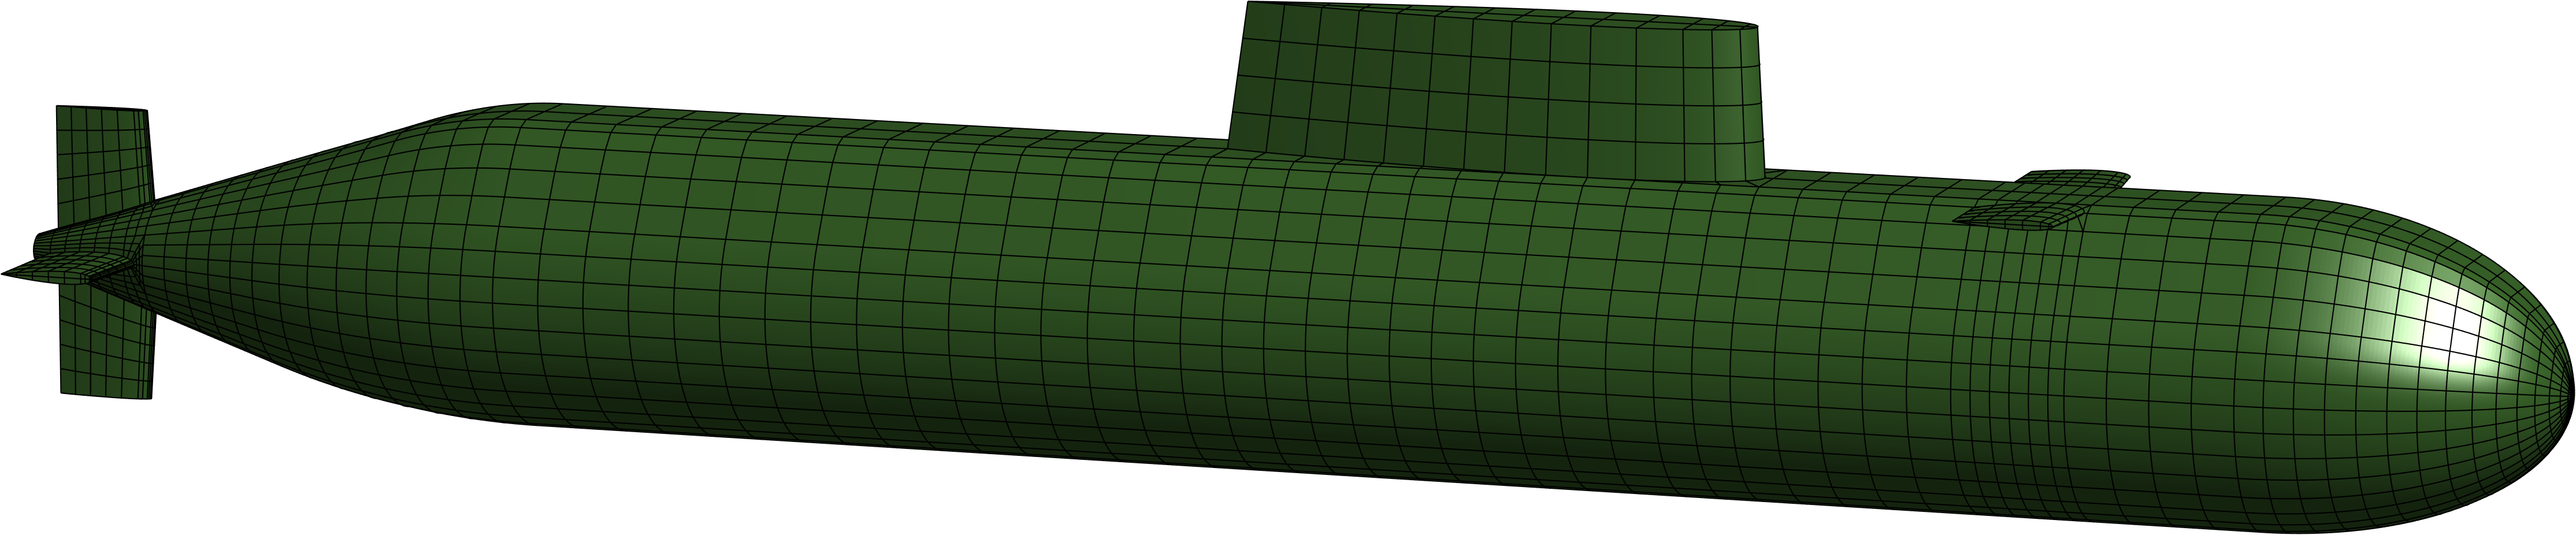
\includegraphics[width=\textwidth]{mesh1}
		\caption{Mesh 1.}
	\end{subfigure}%
	\hspace*{0.02\textwidth}%
	\begin{subfigure}{0.49\textwidth}
		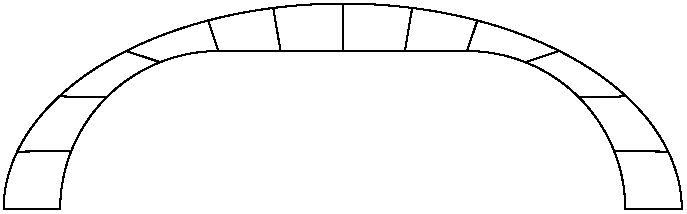
\includegraphics[width=\textwidth]{mesh3}
		\caption{Mesh 3.}
	\end{subfigure}
	\par\bigskip
	\begin{subfigure}{0.49\textwidth}
		\centering
		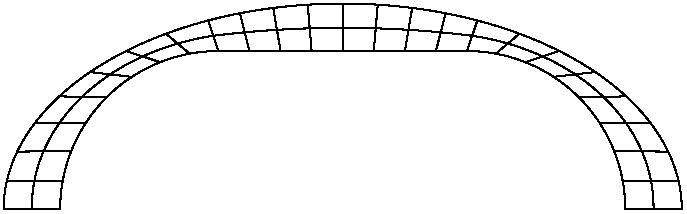
\includegraphics[width=\textwidth]{mesh4}
		\caption{Mesh 4.}
	\end{subfigure}%
	\hspace*{0.02\textwidth}%
	\begin{subfigure}{0.49\textwidth}
		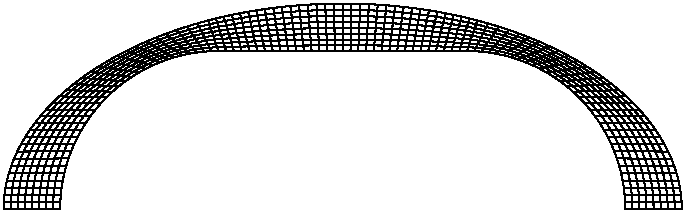
\includegraphics[width=\textwidth]{mesh6}
		\caption{Mesh 6.}
	\end{subfigure}
	\caption{\textbf{Radial pulsation from a mock shell}: Meshes for the fluid domain between the scatterer and the artificial boundary. The meshes are constructed from the initial mesh 1, which is rotated around the axis of symmetry using four elements. Mesh 2 and 3 are refined only in the angular direction, while the more refined meshes also refine in the radial direction to obtain smallest aspect ratio. The meshes are nested.}
	\label{Fig2:MS_meshes}
\end{figure}
\begin{figure}
	\centering
	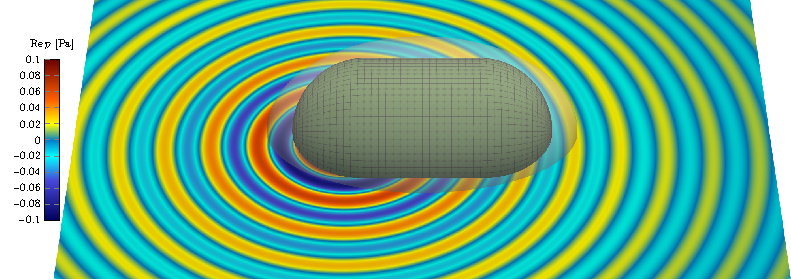
\includegraphics[width=\textwidth]{MS_PnearField}
	\caption{\textbf{Radial pulsation from a mock shell}: Visualization of numerical solution in the $xy$-plane using BGU with $N=6$ on mesh 5.}
	\label{Fig2:MS_visualization}
\end{figure}
Convergence plots are shown in \Cref{Fig2:MS_convergence}. Gerdes did a similar comparison in~\cite{Gerdes1998tcv} where scattering on a sphere was investigated. Our results verify these findings, namely lower errors for the unconjugated formulations (cf. \Cref{Fig2:MS_convergence}). Good results can be obtained using only a single radial shape function in case of unconjugated formulations. For the conjugated versions, on the other hand, $N > 6$ functions are needed to obtain similar accuracy and more degrees of freedom are required to get an asymptotic behavior.

In \Cref{Fig2:MS_condNumbersB} and \Cref{Fig2:MS_condNumbersP} the condition number is investigated for the different formulations and basis functions in the radial shape functions. The condition number for the unconjugated versions increases more rapidly as a function of $N$ compared to the corresponding formulations in the conjugated case. The condition number of the Lagrange basis increases particularly fast with $N$, making it useless\footnote{In the case of $r_n = nr_{\mathrm{a}}$.} for the conjugated formulations. However, the Lagrange basis yields the best result for the unconjugated formulations for small $N$. The Chebyshev basis seems to give the best condition numbers for the conjugated formulations for large $N$ (which is required for acceptable results). The unconjugated formulations perform quite similar, both in terms of the condition numbers and the error. The BGU formulation has the additional advantage of producing symmetric matrices and reduces the memory requirement. 
\begin{figure}
	\centering    
	\begin{subfigure}{0.49\textwidth}
		\centering
		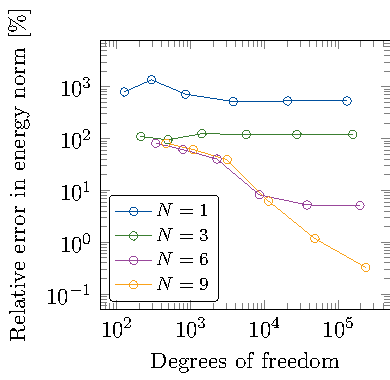
\includegraphics[width=\textwidth]{mockShellConvergence_1}
	\caption{BGC}
	\end{subfigure}%
	\hspace*{0.02\textwidth}%
	\begin{subfigure}{0.49\textwidth}
		\centering
		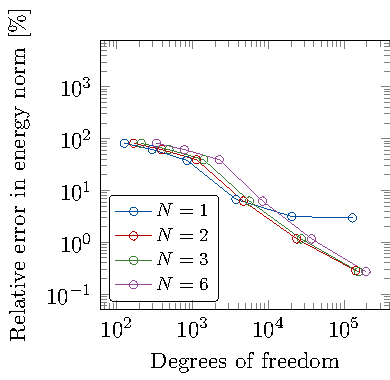
\includegraphics[width=\textwidth]{mockShellConvergence_2}
		\caption{BGU}
	\end{subfigure}%
	\par\bigskip
	\par\bigskip
	\begin{subfigure}{0.49\textwidth}
		\centering
		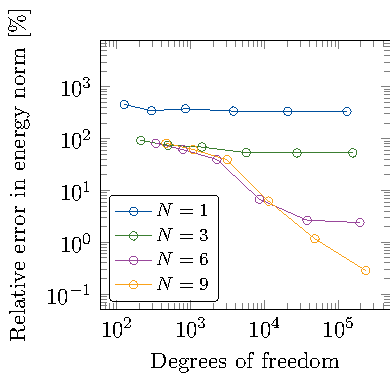
\includegraphics[width=\textwidth]{mockShellConvergence_3}
		\caption{PGC}
	\end{subfigure}%
	\hspace*{0.02\textwidth}%
	\begin{subfigure}{0.49\textwidth}
		\centering
		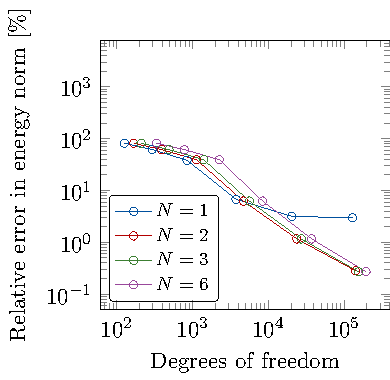
\includegraphics[width=\textwidth]{mockShellConvergence_4}
		\caption{PGU}
	\end{subfigure}%
	\caption{\textbf{Radial pulsation from a mock shell}: Convergence plots for the four infinite element formulations. The relative error in the energy norm (\Cref{Eq2:energyNormFluids}) is plotted against the number of degrees of freedom.}
	\label{Fig2:MS_convergence}
\end{figure}

\begin{figure}
	\begin{subfigure}{0.49\textwidth}
		\centering
		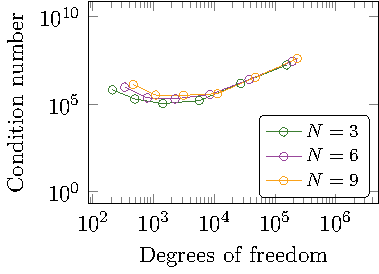
\includegraphics{mockShellConvergence_5}
		\caption{BGC with the shifted Chebyshev basis}
	\end{subfigure}%
	\hspace*{0.02\textwidth}%
	\begin{subfigure}{0.49\textwidth}
		\centering
		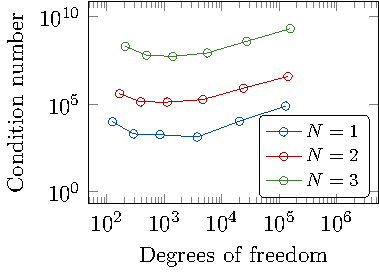
\includegraphics{mockShellConvergence_6}
		\caption{BGU with the shifted Chebyshev basis}
	\end{subfigure}
	\par\bigskip
	\begin{subfigure}{0.49\textwidth}
		\centering
		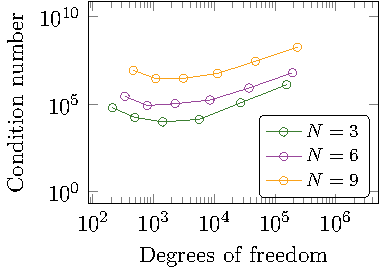
\includegraphics{mockShellConvergence_7}
		\caption{BGC with the Bernstein basis}
	\end{subfigure}%
	\hspace*{0.02\textwidth}%
	\begin{subfigure}{0.49\textwidth}
		\centering
		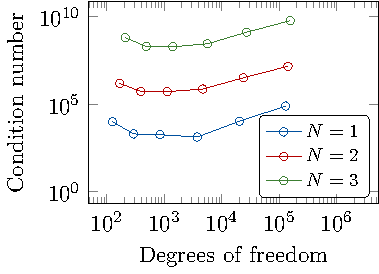
\includegraphics{mockShellConvergence_8}
		\caption{BGU with the Bernstein basis}
	\end{subfigure}
	\par\bigskip
	\begin{subfigure}{0.49\textwidth}
		\centering
		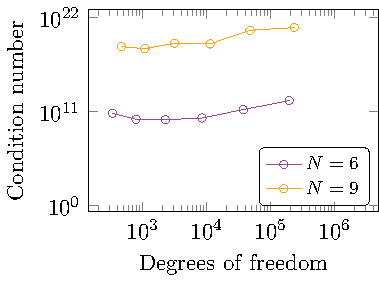
\includegraphics{mockShellConvergence_9}
		\caption{BGC with the Lagrange basis}
	\end{subfigure}%
	\hspace*{0.02\textwidth}%
	\begin{subfigure}{0.49\textwidth}
		\centering
		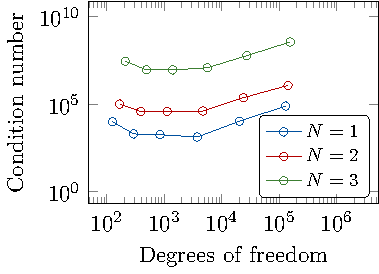
\includegraphics{mockShellConvergence_10}
		\caption{BGU with the Lagrange basis}
	\end{subfigure}
	\caption{\textbf{Radial pulsation from a mock shell}: Convergence plots for the BGC and BGU formulations using three different sets of radial shape functions (Chebyshev, Bernstein and Lagrange). The condition number (1-norm condition number estimate provided by \texttt{condest} in \MATLAB) is plotted against the number of degrees of freedom.}
	\label{Fig2:MS_condNumbersB}
\end{figure}


\begin{figure}
	\begin{subfigure}{0.49\textwidth}
		\centering
		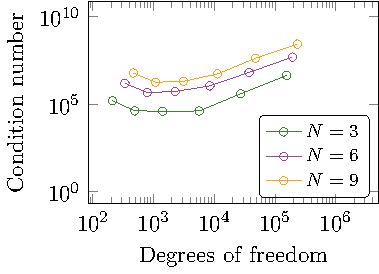
\includegraphics{mockShellConvergence_11}
		\caption{PGC with the shifted Chebyshev basis}
	\end{subfigure}%
	\hspace*{0.02\textwidth}%
	\begin{subfigure}{0.49\textwidth}
		\centering
		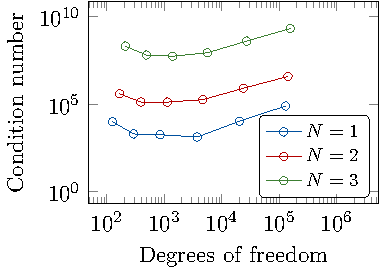
\includegraphics{mockShellConvergence_12}
		\caption{PGU with the shifted Chebyshev basis}
	\end{subfigure}
	\par\bigskip
	\begin{subfigure}{0.49\textwidth}
		\centering
		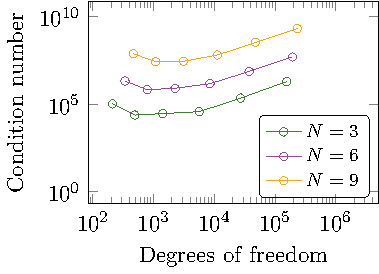
\includegraphics{mockShellConvergence_13}
		\caption{PGC with the Bernstein basis}
	\end{subfigure}%
	\hspace*{0.02\textwidth}%
	\begin{subfigure}{0.49\textwidth}
		\centering
		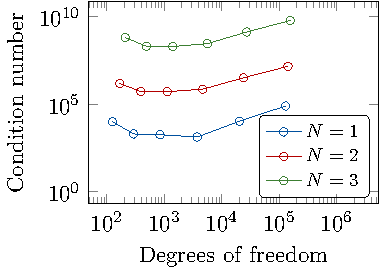
\includegraphics{mockShellConvergence_14}
		\caption{PGU with the Bernstein basis}
	\end{subfigure}
	\par\bigskip
	\begin{subfigure}{0.49\textwidth}
		\centering
		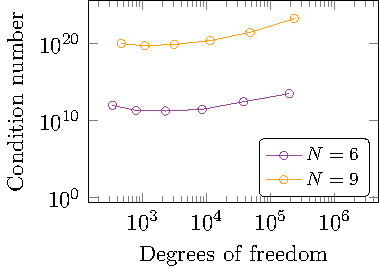
\includegraphics{mockShellConvergence_15}
		\caption{PGC with the Lagrange basis}
	\end{subfigure}%
	\hspace*{0.02\textwidth}%
	\begin{subfigure}{0.49\textwidth}
		\centering
		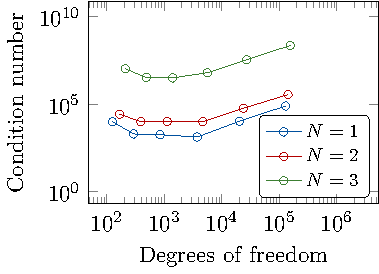
\includegraphics{mockShellConvergence_16}
		\caption{PGU with the Lagrange basis}
	\end{subfigure}
	\caption{\textbf{Radial pulsation from a mock shell}: Convergence plots for the PGC and PGU formulations using three different sets of radial shape functions (Chebyshev, Bernstein and Lagrange). The condition number (1-norm condition number estimate provided by \texttt{condest} in \MATLAB) is plotted against the number of degrees of freedom.}
	\label{Fig2:MS_condNumbersP}
\end{figure}

It is clear that the choice of basis functions in the infinite elements plays a crucial role for the condition number, and more research is required to find the optimal set of basis functions. Based on the findings in this work, it is recommended to use the BGU formulation alongside the Lagrange basis (in the radial direction) in the infinite elements. However, if larger $N$ is needed for accuracy, the Chebyshev basis is recommended.

\subsection{Stripped BeTSSi submarine}
Finally, we consider the \textit{stripped BeTSSi submarine}\footnote{Based upon the BeTSSi submarine which originates from the BeTSSi workshops~\cite{Gilroy2013bib}.} described in \Cref{Sec2:BeTSSi_description}. 

Let a plane wave, with the direction of incidence given by
\begin{equation}
	\vec{d}_{\mathrm{s}} = -\begin{bmatrix}
		\cos\beta_{\mathrm{s}}\cos\alpha_{\mathrm{s}}\\
		\cos\beta_{\mathrm{s}}\sin\alpha_{\mathrm{s}}\\
		\sin\beta_{\mathrm{s}}
	\end{bmatrix}, \quad\text{where}\quad \alpha_{\mathrm{s}} = \ang{240},\,\beta_{\mathrm{s}} = \ang{0},
\end{equation}
be scattered by this submarine. The CAD model is given in \Cref{Fig2:BC_strippedAndMesh} alongside computational meshes. Again, we shall denote by ${\cal M}_{m,\check{p},\check{k}}^{\textsc{iga}}$, mesh number $m$ with polynomial order $\check{p}$ and continuity $\check{k}$ across element boundaries of the NURBS parametrization. 

\begin{figure}
	\begin{subfigure}{\textwidth}
		\centering
		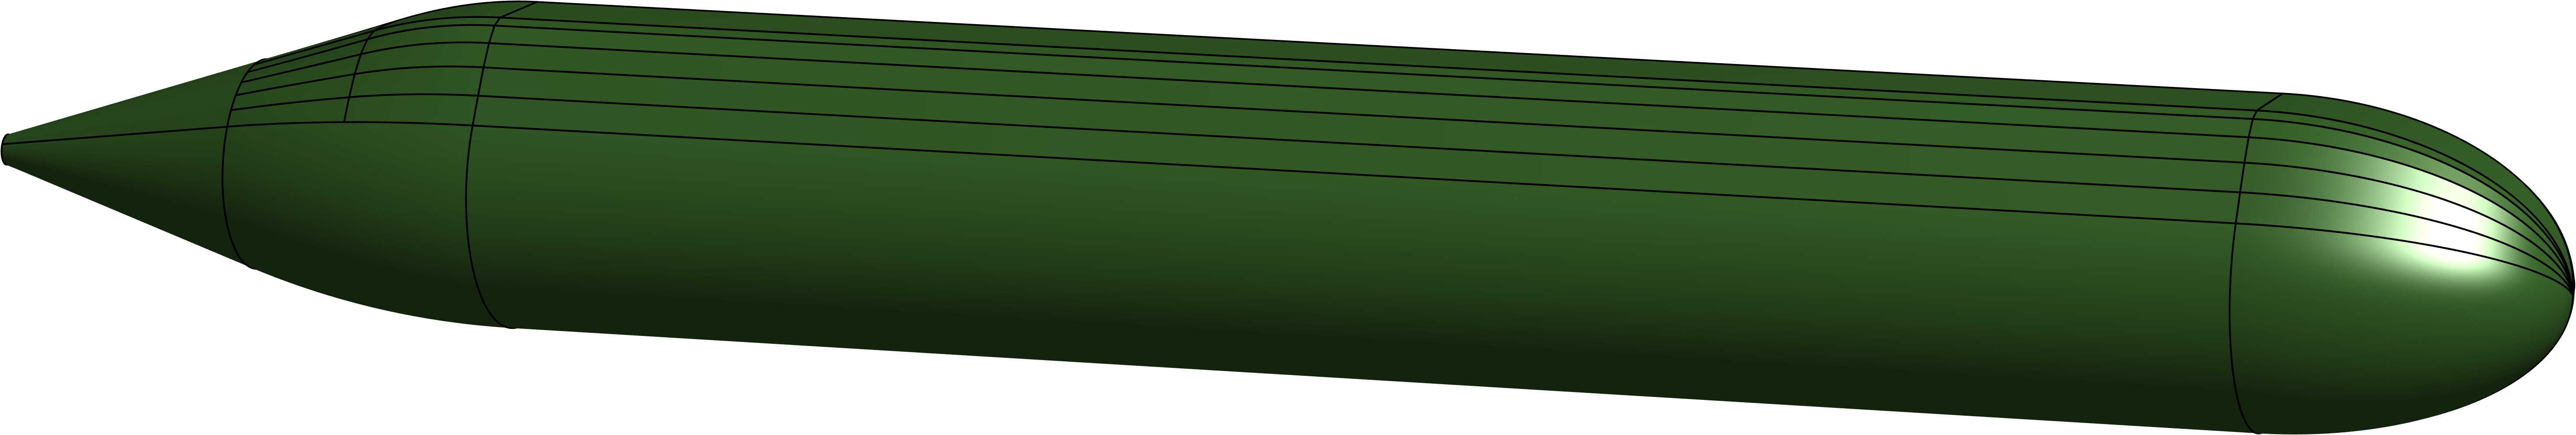
\includegraphics[width=0.95\textwidth]{BeTSSi_BC_stripped}
		\caption{CAD model.}
		\label{Fig2:BC_stripped}
	\end{subfigure}
	\par\bigskip
	\par\bigskip
	\begin{subfigure}{\textwidth}
		\centering
		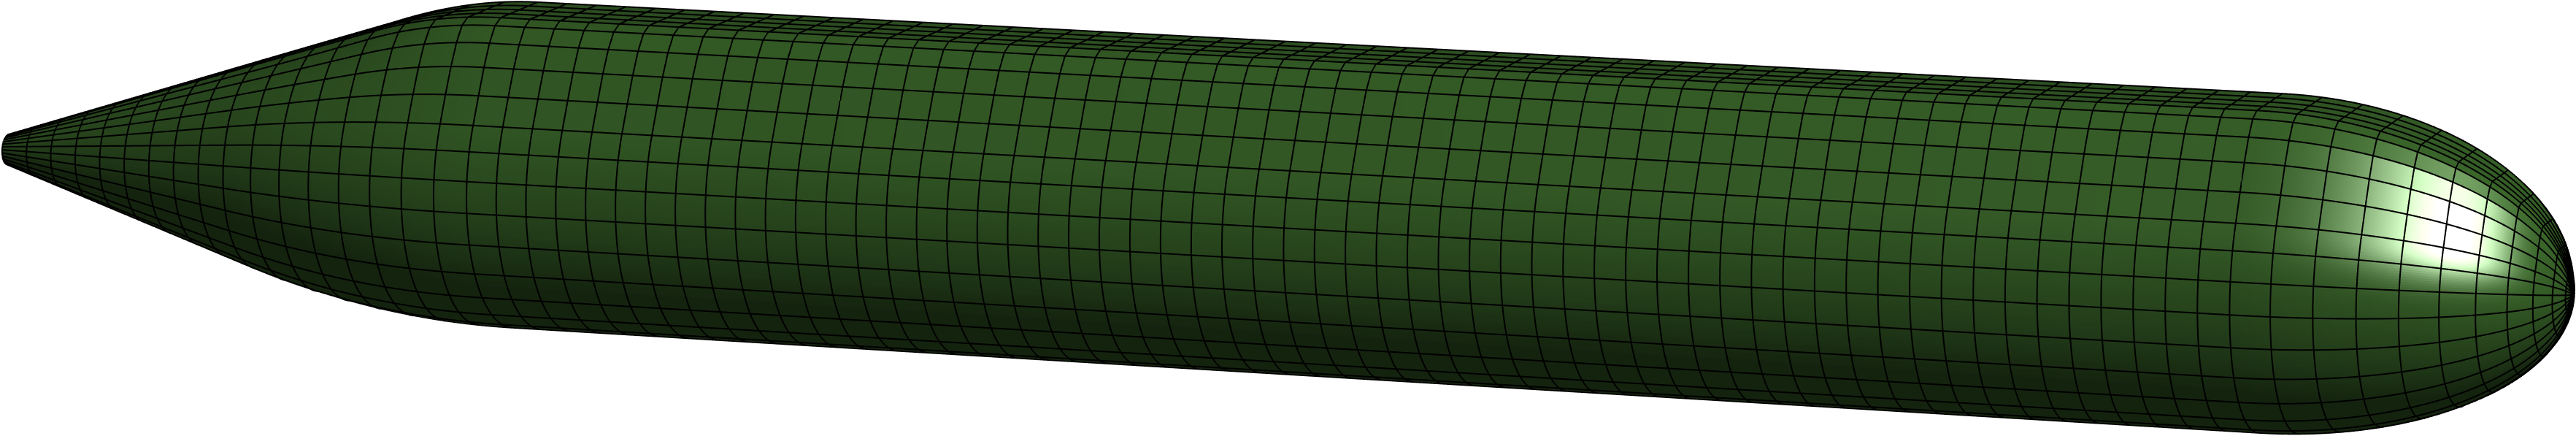
\includegraphics[width=0.95\textwidth]{BeTSSi_BC_mesh1}
		\caption{Surface mesh for mesh ${\cal M}_{1,\check{p},\check{k}}^{\mathrm{IGA}}$}
	\end{subfigure}	
	\par\bigskip
	\par\bigskip
	\begin{subfigure}{\textwidth}
		\centering
		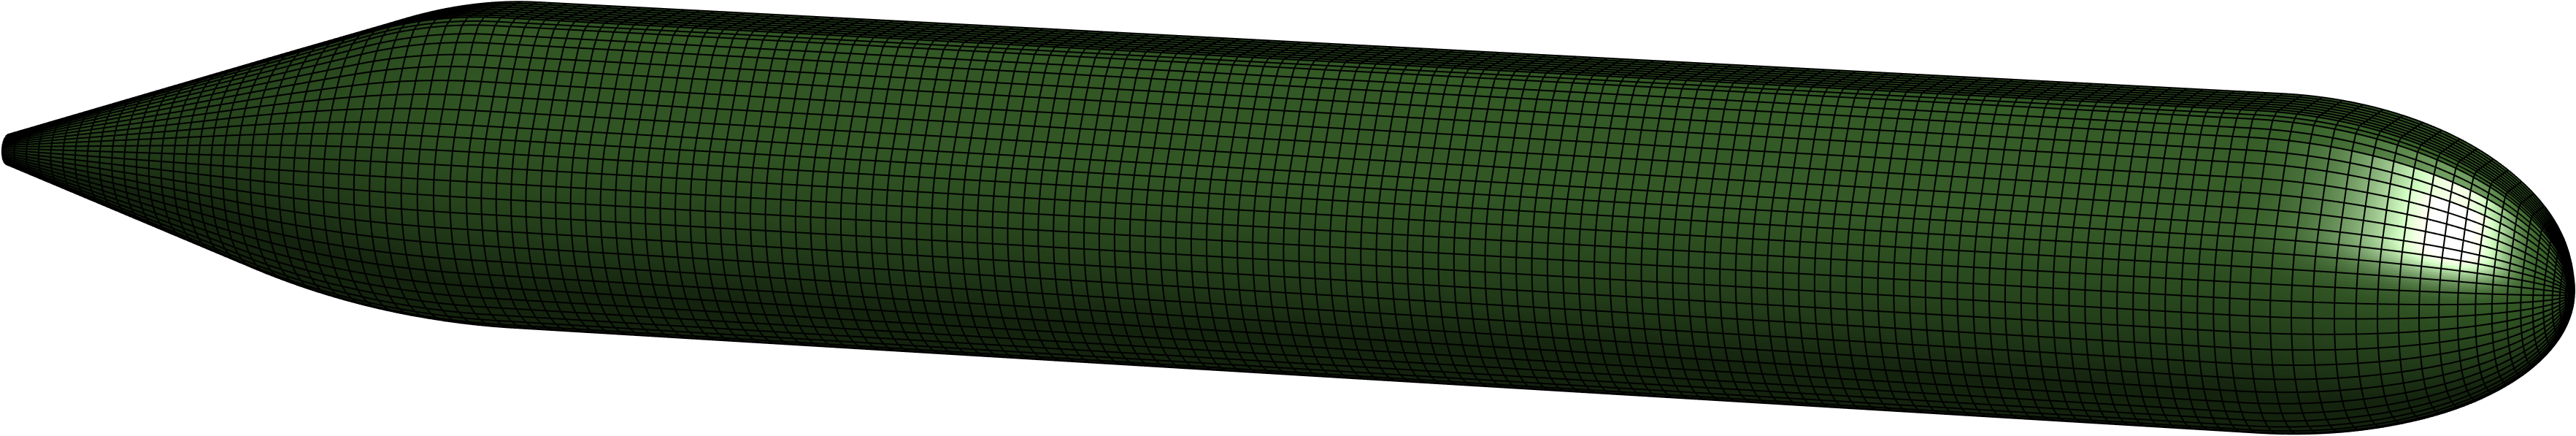
\includegraphics[width=0.95\textwidth]{BeTSSi_BC_mesh2}
		\caption{Surface mesh for mesh ${\cal M}_{2,\check{p},\check{k}}^{\mathrm{IGA}}$.}
	\end{subfigure}	
	\par\bigskip
	\par\bigskip
	\begin{subfigure}{\textwidth}
		\centering
		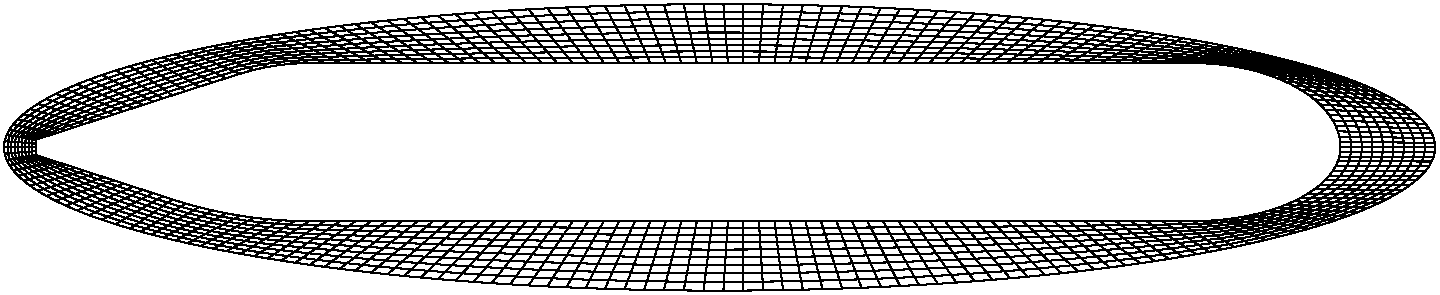
\includegraphics[width=0.95\textwidth]{BeTSSi_BC_mesh1_eta}
		\caption{Crossection in the $xz$-plane for mesh ${\cal M}_{1,\check{p},\check{k}}^{\mathrm{IGA}}$.}
	\end{subfigure}	
	\par\bigskip
	\par\bigskip
	\begin{subfigure}{\textwidth}
		\centering
		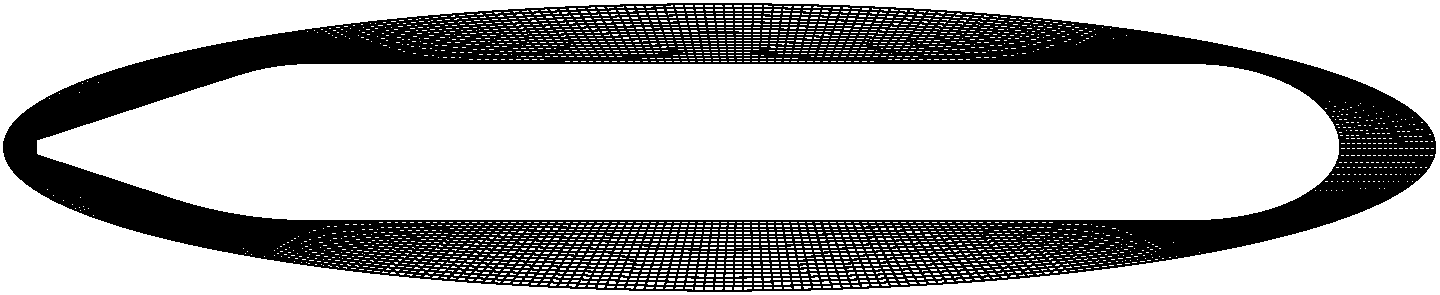
\includegraphics[width=0.95\textwidth]{BeTSSi_BC_mesh2_eta}
		\caption{Crossection in the $xz$-plane for mesh ${\cal M}_{2,\check{p},\check{k}}^{\mathrm{IGA}}$.}
	\end{subfigure}	
	\caption{\textbf{Stripped BeTSSi submarine}: CAD model and meshes used for computations.}
	\label{Fig2:BC_strippedAndMesh}
\end{figure}
The near field at $f=\SI{1000}{Hz}$ is visualized in \Cref{Fig2:BC_NearField}.
\begin{figure}
	\centering    
	\begin{subfigure}[b]{\textwidth}
		\centering
		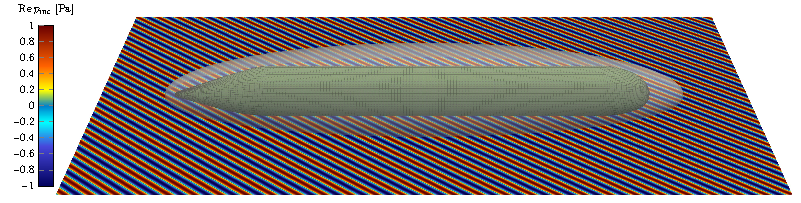
\includegraphics[width=\textwidth]{BC_nearField_1}
		\caption{Real part of the incident wave $p_{\mathrm{inc}}(\vec{x})=P_{\mathrm{inc}}\euler^{\imag k\vec{d}_{\mathrm{s}}\cdot \vec{x}}$.}
	\end{subfigure}
	\par\bigskip
	\begin{subfigure}[b]{\textwidth}
		\centering
		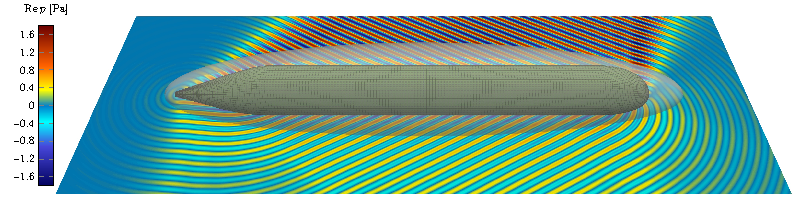
\includegraphics[width=\textwidth]{BC_nearField_2}
		\caption{Real part of the scattered pressure $p(\vec{x})$.}
	\end{subfigure}
	\par\bigskip
	\begin{subfigure}[b]{\textwidth}
		\centering
		\includegraphics[width=\textwidth]{BC_nearField_3}
		\caption{Real part of the total pressure $p_{\mathrm{tot}}(\vec{x})=p_{\mathrm{inc}}(\vec{x})+p(\vec{x})$.}
	\end{subfigure}
	\par\bigskip
	\begin{subfigure}[b]{\textwidth}
		\centering
		\includegraphics[width=\textwidth]{BC_nearField_4}
		\caption{Modulus of the total pressure $p_{\mathrm{tot}}(\vec{x})=p_{\mathrm{inc}}(\vec{x})+p(\vec{x})$.}
	\end{subfigure}
	\caption{\textbf{Stripped BeTSSi submarine with SHBC}: The simulation at $f=\SI{1000}{Hz}$ is visualized in the $xy$-plane, and is computed on mesh ${\cal M}_{2,3,2}^{\mathrm{IGA}}$ and the BGU formulation with $N=4$. The numerical evaluations outside the (transparent) prolate ellipsoidal artificial boundary are evaluated with \Cref{Eq2:KirchhoffIntegral}.}
	\label{Fig2:BC_NearField}
\end{figure}
The low frequency problem at $f = \SI{100}{Hz}$ is considered in~\Cref{Fig2:FarField100}. In this case, mesh ${\cal M}_{1,2,1}^{\mathrm{IGA}}$ resolves this frequency, but the solution slightly deviates from the reference solution computed by IGABEM on a fine mesh. The reason for this is that $N$ is too low. Although $N=3$ was enough for engineering precision (below 1\%) in the mock shell example, it does not suffice for the more complicated geometry like the stripped BeTSSi submarine. Consider the relative error for the far field at the well resolved mesh ${\cal M}_{2,3,2}^{\mathrm{IGA}}$. In this case the error will originate from the low resolution (governed by $N$) in the radial direction for the infinite elements. As illustrated in \Cref{Fig2:FarField100error} an order of magnitude in accuracy is gained by increasing $N$. This effect was also observed by the verification test in \Cref{Subsec2:mockShell} applied to the stripped BeTSSi submarine.
\begin{figure}
	\centering    
	\includegraphics[width=\textwidth]{BC_farField100_1}
	\caption{\textbf{Stripped BeTSSi submarine with SHBC}: Computation of target strength (\Cref{Eq2:TS}) at $f=\SI{100}{Hz}$ as a function of the azimuth angle in the spherical coordinate system. The two IGA results (both using $N=3$) are visually indistinguishable meaning that mesh ${\cal M}_{1,2,1}^{\mathrm{IGA}}$ is well resolved for this frequency.}
	\label{Fig2:FarField100}
\end{figure}
\begin{figure}
	\centering    
	\includegraphics[width=\textwidth]{BC_farField100_2}
	\caption{\textbf{Stripped BeTSSi submarine with SHBC}: Computation of the relative error in the far field (\Cref{Eq2:KirchhoffIntegral}) compared to a reference solution at $f=\SI{100}{Hz}$. The computations are done using IGA on mesh ${\cal M}_{2,3,2}^{\mathrm{IGA}}$ using the BGU formulation.}
	\label{Fig2:FarField100error}
\end{figure}
In \Cref{Fig2:FarField} the target strength is plotted for $f=\SI{500}{Hz}$ and $f=\SI{1000}{Hz}$. A reference solution (using IGABEM) is added for the $f=\SI{500}{Hz}$ case, and illustrates again the pollution of low $N$. The IGA mesh 1 resolves the frequency $f=\SI{500}{Hz}$ quite well using only about 5 elements per wavelength. This corresponds to about 5 dofs per wavelength in each dimensional direction compared to the classical 10-12 dofs per wavelength needed for FEM methods.
\begin{figure}
	\centering    
	\begin{subfigure}[b]{\textwidth}
		\centering
		\includegraphics[width=\textwidth]{BC_farField_1}
		\caption{$f=\SI{500}{Hz}$}
	\end{subfigure}
	\par\bigskip
	\par\bigskip
	\begin{subfigure}[b]{\textwidth}
		\centering
		\includegraphics[width=\textwidth]{BC_farField_2}
		\caption{$f=\SI{1000}{Hz}$}
	\end{subfigure}
	\caption{\textbf{Stripped BeTSSi submarine with SHBC}: Computation of target strength (\Cref{Eq2:TS}) as a function of the azimuth angle in the spherical coordinate system. The numerical evaluations are evaluated with \Cref{Eq2:TS}.}
	\label{Fig2:FarField}
\end{figure}

%\clearpage
\section{Conclusion}
\label{Sec4:conclusions}
This article addresses acoustic scattering characterized by sound waves reflected by man-made elastic objects. The present approach is characterized by:
\begin{itemize}
	\item The scattered pressure is approximated by Kirchhoff approximation.
	\item The computations are evaluated on the exact computer aided design model.
	\item The Helmholtz integrals are evaluated by the numerical steepest descent.
\end{itemize}

The main finding of the present study is that Kirchhoff approximation may be computed with a complexity independent of the frequency in the isogeometric analysis framework.

Furthermore, the following observations are made
\begin{itemize}
	\item The accuracy of the method converges as a function of the frequency, as opposed to a triangular approximation method where the accuracy diverges.
	\item The computational complexity of the Kirchhoff approximation method is at least one order less than finite/boundary element methods resulting in computational savings in orders of magnitudes. The cost of these savings is reduced accuracy, and for some geometries the Kirchhoff approximation simply is not applicable.
	\item The NSD formulation outperforms the triangulation approximation approach when considering the computational time as a function of the error or frequency.
\end{itemize}

The Kirchhoff approximation method in an isogeometric framework has good potential, but many challenges remains to be resolved before the presented code is fully automated.

Some challenges remain to be resolved for this work to be applicable to general CAD geometries. First, for each incident wave and for each element in the CAD mesh, all resonance and stationary points must be found. This could be implemented as a preprocessing step. Second, if the shadow boundary does not coincide with element boundaries, this must be resolved in the NSD algorithm. The parent domain will in this case not be rectangular, but rather parametrized boundary which requires special treatment in the NSD algorithm. Moreover, this challenge will affect the first challenge as potential resonance points may lie on the shadow boundary. Third, interior stationary points have not been considered in this work but is discussed in~\cite{Huybrechs2007tco}. Finally, rules must be established for the number of Gauss-Legendre points and Gauss-Laguerre points needed in the hybrid method.

To have an automated algorithm that tackles all of these challenges is a huge task. The integrals from the usage of curvilinear facets in~\cite{Lavia2018mhf} contains well behaved oscillatory functions ($g$ is second order polynomial) and may for this reason be a simpler approach. Especially since it is easier to discretize the scatterer, $\Gamma$, with curvilinear triangles in such a way that the shadow boundary lies on element edges.

\section*{Acknowledgements}
This work was supported by the Department of Mathematical Sciences at the Norwegian University of Science and Technology and by the Norwegian Defence Research Establishment.

We would like to thank Arieh Iserles for hosting us at our research stay at the Department of Applied Mathematics and Theoretical Physics at University of Cambridge (UK) during the fall of 2016. His guidance related to highly oscillatory integration is highly appreciated. We would also like to thank Daan Huybrechs at K.U. Leuven University (Belgium) for valuable comments about the numerical steepest descent method. 

%\clearpage
%
\begin{inputAppendices}
\newpage
\section{Derivation of bilinear form in infinite elements}
\label{Sec2:AppendixDerivationOfBilinearForm}
In this appendix, the integrals in the bilinear forms for the infinite elements will be separated for the PGU case\footnote{The other three formulations have been derived in~\cite{Venas2015iao}. For the more general ellipsoidal coordinate system, refer to~\cite{Burnett1998aea}.}. For generality, the derivation is done in the prolate spheroidal coordinate system.

\subsection{The prolate spheroidal coordinate system}
\label{Sec2:prolateSphericalCoordinateSystem}
The prolate spheroidal coordinate system is an extension of the spherical coordinate system. It is defined by the relations
\begin{align}
	x &= \sqrt{r^2 - \Upsilon^2}\sin\vartheta\cos\varphi\\
	y &= \sqrt{r^2 - \Upsilon^2}\sin\vartheta\sin\varphi\\
	z &= r\cos\vartheta
\end{align}
with foci located at $z = \pm \Upsilon$ and $r\geq \Upsilon$. Note that the coordinate system reduces to the spherical coordinate system when $\Upsilon=0$. the following inverse formulas may be derived
\begin{align}\label{Eq2:XtoProl}
\begin{split}
	r &= \frac{1}{2}(d_1+d_2)\\
	\vartheta &= \arccos\left(\frac{z}{r}\right)\\
	\varphi &= \operatorname{atan2}(y,x)
\end{split}
\end{align}
where 
\begin{align*}
	d_1 &= d_1(x,y,z) = \sqrt{x^2+y^2+(z+\Upsilon)^2}\\
	d_2 &= d_2(x,y,z) = \sqrt{x^2+y^2+(z-\Upsilon)^2}
\end{align*}
and 
\begin{equation*}
	\operatorname{atan2}(y,x) = \begin{cases}
	\arctan(\frac{y}{x}) & \mbox{if } x > 0\\
	\arctan(\frac{y}{x}) + \PI & \mbox{if } x < 0 \mbox{ and } y \ge 0\\
	\arctan(\frac{y}{x}) - \PI & \mbox{if } x < 0 \mbox{ and } y < 0\\
	\frac{\PI}{2} & \mbox{if } x = 0 \mbox{ and } y > 0\\
	-\frac{\PI}{2} & \mbox{if } x = 0 \mbox{ and } y < 0\\
	\text{undefined} & \mbox{if } x = 0 \mbox{ and } y = 0.
	\end{cases}
\end{equation*}
The derivatives are found to be
\begin{equation}\label{Eq2:dXdProlateSphericalCoordinates}
\begin{alignedat}{4}
	\pderiv{x}{r} &= \frac{r\sin\vartheta\cos\varphi}{\sqrt{r^2-\Upsilon^2}},\qquad	&&\pderiv{y}{r} = \frac{r\sin\vartheta\sin\varphi}{\sqrt{r^2-\Upsilon^2}},\qquad	&&\pderiv{z}{r} = \cos\vartheta\\
	\pderiv{x}{\vartheta} &=\sqrt{r^2-\Upsilon^2}\cos\vartheta\cos\varphi,\qquad	&&\pderiv{y}{\vartheta} = \sqrt{r^2-\Upsilon^2}\cos\vartheta\sin\varphi,\qquad	&&\pderiv{z}{\vartheta} = -r\sin\vartheta\\
	\pderiv{x}{\varphi} &= -\sqrt{r^2-\Upsilon^2}\sin\vartheta\sin\varphi,\qquad	&&\pderiv{y}{\varphi} = \sqrt{r^2-\Upsilon^2}\sin\vartheta\cos\varphi,\qquad	&&\pderiv{z}{\varphi} =0
\end{alignedat}
\end{equation}
and
\begin{equation}\label{Eq2:dProlateSphericalCoordinatesdX}
\begin{aligned}
	\pderiv{r}{x} &= \frac{x(d_1+d_2)}{2d_1d_2},\qquad	\pderiv{r}{y} = \frac{y(d_1+d_2)}{2d_1d_2}\qquad\\
	\pderiv{r}{z} &= \frac{z(d_1+d_2)+\Upsilon(d_2-d_1)}{2d_1d_2}\\
	\pderiv{\vartheta}{x} &= \frac{xz}{d_1d_2\sqrt{r^2-z^2}},\qquad	\pderiv{\vartheta}{y} = \frac{yz}{d_1d_2\sqrt{r^2-z^2}}	\\
	\pderiv{\vartheta}{z} &= \frac{1}{\sqrt{r^2-z^2}}\left(\frac{z^2}{d_1d_2}+\frac{\Upsilon z(d_2-d_1)}{d_1d_2(d_1+d_2)}-1\right) \\
	\pderiv{\varphi}{x} &= -\frac{y}{x^2+y^2},\qquad	\pderiv{\varphi}{y} = \frac{x}{x^2+y^2},\qquad	\pderiv{\varphi}{z} = 0.
\end{aligned}
\end{equation}
The general nabla operator can be written as
\begin{equation}\label{Eq2:GeneralNablaOperator}
	\nabla = \frac{\vec{e}_{\mathrm{r}}}{h_{\mathrm{r}}} \pderiv{}{r} + \frac{\vec{e}_{\upvartheta}}{h_{\upvartheta}} \pderiv{}{\vartheta} + \frac{\vec{e}_{\upvarphi}}{h_{\upvarphi}} \pderiv{}{\varphi}
\end{equation}
where
\begin{equation*}
	\vec{e}_{\mathrm{r}} = \frac{1}{h_{\mathrm{r}}}\left[\pderiv{x}{r}, \pderiv{y}{r}, \pderiv{z}{r}\right]^\transpose,\quad
	\vec{e}_{\upvartheta} = \frac{1}{h_{\upvartheta}}\left[\pderiv{x}{\vartheta}, \pderiv{y}{\vartheta}, \pderiv{z}{\vartheta}\right]^\transpose,\quad
	\vec{e}_{\upvarphi} = \frac{1}{h_{\upvarphi}}\left[\pderiv{x}{\varphi}, \pderiv{y}{\varphi}, \pderiv{z}{\varphi}\right]^\transpose
\end{equation*}
and
\begin{align*}
	h_{\mathrm{r}} &= \sqrt{\frac{r^2-\Upsilon^2\cos^2\vartheta}{r^2-\Upsilon^2}}\\
	h_{\upvartheta} &= \sqrt{r^2-\Upsilon^2\cos^2\vartheta}\\
	h_{\upvarphi} &= \sqrt{r^2-\Upsilon^2}\sin\vartheta.
\end{align*}
The Jacobian determinant (for the mapping from Cartesian coordinates to prolate spheroidal coordinates) may now be written as
\begin{equation}
	J_1 = h_{\mathrm{r}} h_{\upvartheta} h_{\upvarphi} = \left(r^2-\Upsilon^2\cos^2\vartheta\right)\sin\vartheta.
\end{equation}
As any normal vector at a surface with constant radius $r=\gamma$ can be written as $\vec{n} = \vec{e}_{\upvartheta}\times\vec{e}_{\upphi}=\vec{e}_{\mathrm{r}}$
\begin{equation}
	\partial_n p = \vec{n}\cdot\nabla p = \vec{e}_{\mathrm{r}}\cdot\nabla p = \frac{1}{h_{\mathrm{r}}} \pderiv{p}{r}.
\end{equation}
The surface Jacobian determinant at a given (constant) $r=\gamma$ is
\begin{equation}
	J_S = h_{\upvartheta} h_{\upvarphi} = \sqrt{r^2-\Upsilon^2\cos^2\vartheta}\sqrt{r^2-\Upsilon^2}\sin\vartheta,
\end{equation}
such that
\begin{equation}
	q\partial_n p J_S = \bigoh\left(r^{-3}\right)\quad\text{whenever}\quad q=\bigoh\left(r^{-3}\right)\quad\text{and}\quad p = \bigoh\left(r^{-1}\right).
\end{equation}
That is, for the Petrov--Galerkin formulations
\begin{equation}
	\lim_{\gamma\to\infty}\int_{S^\gamma} q\partial_n p\idiff\Gamma = \lim_{\gamma\to\infty}\int_0^{2\PI}\int_0^\PI q\partial_n p J_S\idiff\vartheta\idiff\varphi = 0.
\end{equation}

\subsection{Bilinear form for unconjugated Petrov--Galerkin formulation}
The bilinear form (in the domain outside the artificial boundary) in~\Cref{Eq2:B_uc_a} (in the unconjugated case) can in the Petrov--Galerkin formulations be simplified to
\begin{align}\label{Eq2:BilinearFormInserted}
	\begin{split}
	B_{\textsc{pgu}}(R_I\psi_n,R_J\phi_m) &= \lim_{\gamma\to\infty}\int_{\Omega_{\mathrm{a}}^\gamma} \left[\nabla(R_I\psi_n)\cdot \nabla (R_J\phi_m)- k^2 R_I\psi_n R_J\phi_m\right]\idiff\Omega\\
		&=\int_{\Omega_{\mathrm{a}}^+} \left[\nabla(R_I\psi_n)\cdot \nabla (R_J\phi_m)- k^2 R_I\psi_n R_J\phi_m\right]\idiff\Omega
	\end{split}
\end{align}
as the mentioned surface integral in the far field vanishes (this is however not the case for the Bubnov--Galerkin formulations). Recall that the radial shape functions are given by
\begin{align*}
	\phi_m(r) &= \euler^{\imag k (r-r_{\mathrm{a}})}Q_m\left(\frac{r_{\mathrm{a}}}{r}\right),\quad m = 1,\dots,N\\
	\psi_n(r) &= \euler^{\imag k (r-r_{\mathrm{a}})}\tilde{Q}_n\left(\frac{r_{\mathrm{a}}}{r}\right),\quad n = 1,\dots,N
\end{align*}
such that the derivative can be computed by
\begin{equation*}
	\deriv{\phi_m}{r} = \left[\imag kQ_m\left(\frac{r_{\mathrm{a}}}{r}\right) - \frac{r_{\mathrm{a}}}{r^2}Q_m'\left(\frac{r_{\mathrm{a}}}{r}\right)\right]\euler^{\imag k (r-r_{\mathrm{a}})}
\end{equation*}
and corresponding expression for $\psi_n$. Using the expression for the nabla operator found in \Cref{Eq2:GeneralNablaOperator}
\begin{align*}
	\nabla(R_I\psi_n)\cdot \nabla (R_J\phi_m) &= \frac{1}{h_{\mathrm{r}}^2}\pderiv{(R_I\psi_n)}{r}\pderiv{(R_J\phi_m)}{r} + \frac{1}{h_{\uptheta}^2}\pderiv{(R_I\psi_n)}{\vartheta}\pderiv{(R_J\phi_m)}{\vartheta} \\
	&{\hskip6em\relax}+ \frac{1}{h_{\upvarphi}^2}\pderiv{(R_I\psi_n)}{\varphi}\pderiv{(R_J\phi_m)}{\varphi}\\
	 &= \frac{1}{h_{\mathrm{r}}^2}\pderiv{\psi_n}{r}\pderiv{\phi_m}{r}R_IR_J + \frac{1}{h_{\uptheta}^2}\psi_n\phi_m\pderiv{R_I}{\vartheta}\pderiv{R_J}{\vartheta}\\
	 &{\hskip6em\relax}+ \frac{1}{h_{\upvarphi}^2}\psi_n\phi_m\pderiv{R_I}{\varphi}\pderiv{R_J}{\varphi}
\end{align*}
which multiplied with the Jacobian $J_1$ yields
\begin{align*}
	\nabla(R_I\psi_n)\cdot \nabla (R_J\phi_m) J_1&= \left[\left(r^2-\Upsilon^2\right)\pderiv{\psi_n}{r}\pderiv{\phi_m}{r}R_IR_J + \psi_n\phi_m\pderiv{R_I}{\vartheta}\pderiv{R_J}{\vartheta}\right. \\
	 &{\hskip8em\relax}\left.+ \frac{r^2-\Upsilon^2\cos^2\vartheta}{(r^2-\Upsilon^2)\sin^2\vartheta}\psi_n\phi_m\pderiv{R_I}{\varphi}\pderiv{R_J}{\varphi}\right]\sin\vartheta
\end{align*}
Combining all of this into \Cref{Eq2:BilinearFormInserted} yields
\begin{align}
	B_{\textsc{pgu}}(R_I\psi_n,R_J\phi_m) = &\int_0^{2\PI}\int_0^\PI K(\vartheta,\varphi)\sin\vartheta\idiff\vartheta\idiff\varphi
\end{align}
where
\begin{align*}
	K(\vartheta,\varphi) &= \int_{r_{\mathrm{a}}}^{\infty} \left\{\left(r^2-\Upsilon^2\right)\pderiv{\psi_n}{r}\pderiv{\phi_m}{r}R_IR_J + \psi_n\phi_m\pderiv{R_I}{\vartheta}\pderiv{R_J}{\vartheta}\right. \\
	 &{\hskip4em\relax}\left.+ \frac{r^2-\Upsilon^2\cos^2\vartheta}{(r^2-\Upsilon^2)\sin^2\vartheta}\psi_n\phi_m\pderiv{R_I}{\varphi}\pderiv{R_J}{\varphi}\right.\\
	 &{\hskip4em\relax}\left.-k^2(r^2-\Upsilon^2\cos^2\vartheta)\psi_n\phi_m R_I R_J\right\}\idiff r.
\end{align*}
Inserting the expressions for the radial shape functions $\phi$ and $\psi$ (with Einstein's summation convention) with their corresponding derivatives one obtains the following expression using the substitution $\rho = \frac{r}{r_{\mathrm{a}}}$ and the notation $\varrho_1 = \Upsilon/r_{\mathrm{a}}$ (the eccentricity of the infinite-element spheroid), $\varrho_2=kr_{\mathrm{a}}$ and $\varrho_3=k\Upsilon$
\begin{align*} 
	 K(\vartheta,\varphi) &= \left\{R_IR_J\left[-2\varrho_2^2B_{\tilde{n}+\tilde{m}}^{(1)} - \imag \varrho_2(\tilde{n}+\tilde{m}+2)B_{\tilde{n}+\tilde{m}+1}^{(1)} \phantom{\left(\pderiv{r_{\mathrm{a}}}{\varphi}\right)^2} \right.\right.\\
	 &\left.\left.{\hskip5em\relax} + \left[\tilde{m}(\tilde{n}+2) +\varrho_3^2\right]B_{\tilde{n}+\tilde{m}+2}^{(1)}+ \imag \varrho_1^2\varrho_2(\tilde{n}+\tilde{m}+2)B_{\tilde{n}+\tilde{m}+3}^{(1)}\right.\right.\\
	 &\left.\left.{\hskip5em\relax}  - \tilde{m}(\tilde{n}+2)\varrho_1^2 B_{\tilde{n}+\tilde{m}+4}^{(1)}+\varrho_3^2\cos^2\vartheta B_{\tilde{n}+\tilde{m}+2}^{(1)}\right] \right.\\
	 &\left.{\hskip2em\relax}+ \pderiv{R_I}{\vartheta}\pderiv{R_J}{\vartheta}B_{\tilde{n}+\tilde{m}+2}^{(1)}\right.\\
	 &\left.{\hskip2em\relax}+\pderiv{R_I}{\varphi}\pderiv{R_J}{\varphi}\frac{1}{\sin^2\vartheta}\left(B_{\tilde{n}+\tilde{m}+1}^{(2)} - \varrho_1^2\cos^2\vartheta B_{\tilde{n}+\tilde{m}+3}^{(2)}\right)\right\}r_{\mathrm{a}}\euler^{-2\imag \varrho_2}\tilde{D}_{n\tilde{n}}D_{m\tilde{m}}
\end{align*}
where the radial integrals
\begin{equation*}
	B_{n}^{(1)} = \int_{1}^\infty \frac{\euler^{2\imag \varrho_2 \rho}}{\rho^n}\idiff \rho \qquad B_{n}^{(2)} = \int_{1}^\infty \frac{\euler^{2\imag \varrho_2\rho}}{(\rho^2-\varrho_1^2)\rho^{n-1}}\idiff \rho,\qquad n\geq 1
\end{equation*}
can be evaluated according to formulas in \Cref{Sec2:radIntegrals}.

Assume that the artificial boundary $\Gamma_{\mathrm{a}}$ is parameterized by $\xi$ and $\eta$. As $\Gamma_{\mathrm{a}}$ is a surface with constant radius, $r=r_{\mathrm{a}}$, in the prolate spheroidal coordinate system, it may also be parameterized by $\vartheta$ and $\varphi$. Therefore,
\begin{equation}
	\diff \vartheta\diff\varphi = \begin{vmatrix}
		\pderiv{\vartheta}{\xi} & \pderiv{\varphi}{\xi}\\
		\pderiv{\vartheta}{\eta} & \pderiv{\varphi}{\eta}		
	\end{vmatrix}\diff\xi\diff\eta
\end{equation}
where
\begin{align*}
	\pderiv{\vartheta}{\xi} &= \pderiv{\vartheta}{x}\pderiv{x}{\xi} + \pderiv{\vartheta}{y}\pderiv{y}{\xi} + \pderiv{\vartheta}{z}\pderiv{z}{\xi},\qquad
	\pderiv{\vartheta}{\eta} = \pderiv{\vartheta}{x}\pderiv{x}{\eta} + \pderiv{\vartheta}{y}\pderiv{y}{\eta} + \pderiv{\vartheta}{z}\pderiv{z}{\eta}\\
	\pderiv{\varphi}{\xi} &= \pderiv{\varphi}{x}\pderiv{x}{\xi} + \pderiv{\varphi}{y}\pderiv{y}{\xi} + \pderiv{\varphi}{z}\pderiv{z}{\xi},\qquad
	\pderiv{\varphi}{\eta} = \pderiv{\varphi}{x}\pderiv{x}{\eta} + \pderiv{\varphi}{y}\pderiv{y}{\eta} + \pderiv{\varphi}{z}\pderiv{z}{\eta}
\end{align*}
and the inverse partial derivatives with respect to the coordinate transformation (from the prolate spheroidal coordinate system to the Cartesian coordinate system) is found in \Cref{Eq2:dProlateSphericalCoordinatesdX}. This Jacobian matrix may be evaluated by
\begin{equation}
	J_3 = \begin{bmatrix}
		\pderiv{\vartheta}{\xi} & \pderiv{\vartheta}{\eta}\\
		\pderiv{\varphi}{\xi}	 & \pderiv{\varphi}{\eta}
	\end{bmatrix} = \begin{bmatrix}
		\pderiv{\vartheta}{x} & \pderiv{\vartheta}{y} & \pderiv{\vartheta}{z}\\
		\pderiv{\varphi}{x} & \pderiv{\varphi}{y} & \pderiv{\varphi}{z}
	\end{bmatrix}\begin{bmatrix}
		\pderiv{x}{\xi} & \pderiv{x}{\eta}\\
		\pderiv{y}{\xi} & \pderiv{y}{\eta}\\
		\pderiv{z}{\xi} & \pderiv{z}{\eta}
	\end{bmatrix}
\end{equation}
and the derivatives of the basis functions may then be computed by
\begin{equation}
	\begin{bmatrix}
		\pderiv{R_I}{\vartheta}\\
		\pderiv{R_I}{\varphi}
	\end{bmatrix} = J_3^{-\transpose}\begin{bmatrix}
		\pderiv{R_I}{\xi}\\
		\pderiv{R_I}{\eta}	
	\end{bmatrix}.
\end{equation}
Defining the angular integrals
\begin{equation}\label{Eq2:infiniteElementsSurfaceIntegrals}
\begin{alignedat}{2}
	& A_{IJ}^{(1)} = \int_0^{2\PI}\int_0^\PI R_I R_J\sin\vartheta\idiff\vartheta\idiff\varphi,\qquad\qquad && A_{IJ}^{(2)} = \int_0^{2\PI}\int_0^\PI \pderiv{R_I}{\vartheta} \pderiv{R_J}{\vartheta}\sin\vartheta\idiff\vartheta\idiff\varphi\\
	& A_{IJ}^{(3)} = \int_0^{2\PI}\int_0^\PI R_I R_J\cos^2\vartheta\sin\vartheta\idiff\vartheta\idiff\varphi, \quad && A_{IJ}^{(4)} = \int_0^{2\PI}\int_0^\PI \pderiv{R_I}{\varphi} \pderiv{R_J}{\varphi}\frac{1}{\sin\vartheta}\idiff\vartheta\idiff\varphi\\
	& A_{IJ}^{(5)} = \int_0^{2\PI}\int_0^\PI \pderiv{R_I}{\varphi} \pderiv{R_J}{\varphi}\frac{\cos^2\vartheta}{\sin\vartheta}\idiff\vartheta\idiff\varphi
\end{alignedat}	
\end{equation}
the bilinear form may then finally be written as (Einstein's summation convention is used for the indices $\tilde{n}$ and $\tilde{m}$)
\begin{align}\label{Eq2:finalBilinearFormB_uc_a}
\begin{split}
	&B_{\textsc{pgu}}(R_I\psi_n,R_J\phi_m) \\
	 &= \left\{A_{IJ}^{(1)}\left[-2\varrho_2^2 B_{\tilde{n}+\tilde{m}}^{(1)} - \imag\varrho_2(\tilde{n}+\tilde{m}+2)B_{\tilde{n}+\tilde{m}+1}^{(1)} + \left[(\tilde{n}+2)\tilde{m}+\varrho_3^2\right]B_{\tilde{n}+\tilde{m}+2}^{(1)}\right. \right. \\
	  &{\hskip4em\relax}\left. \left. + \imag\varrho_1\varrho_3(\tilde{n}+\tilde{m}+2)B_{\tilde{n}+\tilde{m}+3}^{(1)} - \varrho_1^2(\tilde{n}+2)\tilde{m}B_{\tilde{n}+\tilde{m}+4}^{(1)}\right] \right. \\
	 &{\hskip2em\relax}\left. +A_{IJ}^{(2)}B_{\tilde{n}+\tilde{m}+2}^{(1)} + \varrho_3^2A_{IJ}^{(3)} B_{\tilde{n}+\tilde{m}+2}^{(1)}\right.\\
	 &{\hskip2em\relax}\left. +A_{IJ}^{(4)}B_{\tilde{n}+\tilde{m}+1}^{(2)} -\varrho_1^2A_{IJ}^{(5)} B_{\tilde{n}+\tilde{m}+3}^{(2)}
	 \right\}r_{\mathrm{a}}\euler^{-2\imag \varrho_2}D_{m\tilde{m}}\tilde{D}_{n\tilde{n}}.
\end{split}
\end{align}
For completeness, the formulas for the other three formulations are included
\begin{equation}
\begin{aligned}
	&B_{\textsc{bgu}}(R_I\psi_n,R_J\phi_m) \\
	 &= \left\{A_{IJ}^{(1)}\left[-2\varrho_2^2 B_{\tilde{n}+\tilde{m}-2}^{(1)}(1-\delta_{\tilde{n}1}\delta_{\tilde{m}1}) - \imag\varrho_2(\tilde{n}+\tilde{m})B_{\tilde{n}+\tilde{m}-1}^{(1)} + \left(\tilde{n}\tilde{m}+\varrho_3^2\right)B_{\tilde{n}+\tilde{m}}^{(1)}\right. \right. \\
	  &{\hskip4em\relax}\left. \left. + \imag\varrho_1\varrho_3(\tilde{n}+\tilde{m})B_{\tilde{n}+\tilde{m}+1}^{(1)} - \varrho_1^2\tilde{n}\tilde{m}B_{\tilde{n}+\tilde{m}+2}^{(1)}\right] \right. \\
	 &{\hskip2em\relax}\left. +A_{IJ}^{(2)}B_{\tilde{n}+\tilde{m}}^{(1)} + \varrho_3^2A_{IJ}^{(3)} B_{\tilde{n}+\tilde{m}}^{(1)}\right.\\
	 &{\hskip2em\relax}\left. +A_{IJ}^{(4)}B_{\tilde{n}+\tilde{m}-1}^{(2)} -\varrho_1^2A_{IJ}^{(5)} B_{\tilde{n}+\tilde{m}+1}^{(2)}
	 \right\}r_{\mathrm{a}}\euler^{-2\imag \varrho_2}D_{m\tilde{m}}\tilde{D}_{n\tilde{n}}\\
	 &\quad-\imag\varrho_2 r_{\mathrm{a}} D_{m1}\tilde{D}_{n1}A_{IJ}^{(1)}
\end{aligned}
\end{equation}
\begin{equation}
\begin{aligned}
	&B_{\textsc{pgc}}(R_I\psi_n,R_J\phi_m) \\
	 &= \left\{A_{IJ}^{(1)}\left[-\imag\varrho_2(\tilde{n}-\tilde{m}+2)B_{\tilde{n}+\tilde{m}+1}^{(1)} + \left[(\tilde{n}+2)\tilde{m}-\varrho_3^2\right]B_{\tilde{n}+\tilde{m}+2}^{(1)}\right. \right. \\
	  &{\hskip4em\relax}\left. \left. + \imag\varrho_1\varrho_3(\tilde{n}-\tilde{m}+2)B_{\tilde{n}+\tilde{m}+3}^{(1)} - \varrho_1^2(\tilde{n}+2)\tilde{m}B_{\tilde{n}+\tilde{m}+4}^{(1)}\right] \right. \\
	 &{\hskip2em\relax}\left. +A_{IJ}^{(2)}B_{\tilde{n}+\tilde{m}+2}^{(1)} + \varrho_3^2A_{IJ}^{(3)} B_{\tilde{n}+\tilde{m}+2}^{(1)}\right.\\
	 &{\hskip2em\relax}\left. +A_{IJ}^{(4)}B_{\tilde{n}+\tilde{m}+1}^{(2)} -\varrho_1^2A_{IJ}^{(5)} B_{\tilde{n}+\tilde{m}+3}^{(2)}
	 \right\}r_{\mathrm{a}}D_{m\tilde{m}}\tilde{D}_{n\tilde{n}}
\end{aligned}
\end{equation}
\begin{equation}
\begin{aligned}
	B_{\textsc{bgc}}(R_I\psi_n,R_J\phi_m) 
	 &= \left\{A_{IJ}^{(1)}\left[-\imag\varrho_2(\tilde{n}-\tilde{m})B_{\tilde{n}+\tilde{m}-1}^{(1)} + \left(\tilde{n}\tilde{m}-\varrho_3^2\right)B_{\tilde{n}+\tilde{m}}^{(1)}\right. \right. \\
	  &{\hskip4em\relax}\left. \left. + \imag\varrho_1\varrho_3(\tilde{n}-\tilde{m})B_{\tilde{n}+\tilde{m}+1}^{(1)} - \varrho_1^2\tilde{n}\tilde{m}B_{\tilde{n}+\tilde{m}+2}^{(1)}\right] \right. \\
	 &{\hskip2em\relax}\left. +A_{IJ}^{(2)}B_{\tilde{n}+\tilde{m}}^{(1)} + \varrho_3^2A_{IJ}^{(3)} B_{\tilde{n}+\tilde{m}}^{(1)}\right.\\
	 &{\hskip2em\relax}\left. +A_{IJ}^{(4)}B_{\tilde{n}+\tilde{m}-1}^{(2)} -\varrho_1^2A_{IJ}^{(5)} B_{\tilde{n}+\tilde{m}+1}^{(2)}
	 \right\}r_{\mathrm{a}}D_{m\tilde{m}}\tilde{D}_{n\tilde{n}}\\
	 &\quad-\imag r_{\mathrm{a}}\varrho_2 D_{m1}\tilde{D}_{n1}A_{IJ}^{(1)} 
\end{aligned}
\end{equation}
where $\delta_{ij}$ is the Kronecker delta function in \Cref{Eq2:Kronecker}.
\section{Evaluation of radial integrals}
\label{Sec2:radIntegrals}
The exponential integral
\begin{equation}
	E_n(z) = \int_1^\infty \frac{\euler^{-z\rho}}{\rho^n}\idiff \rho,\qquad \Re(z) \geq 0
\end{equation}
is of great importance for the unconjugated formulations in the IEM. It is therefore important to be able to evaluate the integral accurately and efficiently, also for large (absolute) values of $z$ (which will correspond to high frequencies). In~\cite[p. 229, 5.1.12]{Abramowitz1965hom} the series representation for evaluation of these functions can be found\footnote{Here, $\upgamma$ is the Euler-Mascheroni constant which is defined by 
\begin{equation*}
\upgamma  = \lim_{n\to\infty}\left[-\ln(n)+\sum_{m=1}^n \frac{1}{m}\right]=0.577215664901532860606512090082\dots.
\end{equation*}}
\begin{equation}\label{Eq2:seriesRepresentation}
	E_n(z) = \frac{(-z)^{n-1}}{(n-1)!}\left[-\ln z-\upgamma+\sum_{m=1}^{n-1}\frac{1}{m}\right] -\sum_{\substack{m=0\\m\neq n-1}}^\infty \frac{(-z)^m}{(m-n+1)m!}
\end{equation}
with the empty sum interpreted to be zero. Moreover, using the continued fraction notation
\begin{equation}
	b_0+\frac{a_1}{b_1+}\frac{a_2}{b_2+}\frac{a_3}{b_3+}\cdots = b_0+\cfrac{a_1}{b_1+\cfrac{a_2}{b_2+\cfrac{a_3}{b_3+\cdots}}}
\end{equation}
the continued fraction representation of these functions is given by~\cite[p. 229, 5.1.22]{Abramowitz1965hom}
\begin{equation}\label{Eq2:contFracRepresentation}
	E_n(z) = \euler^{-z}\left(\frac{1}{z+}\frac{n}{1+}\frac{1}{z+}\frac{n+1}{1+}\frac{2}{z+}\frac{n+2}{1+}\frac{3}{z+}\cdots\right).
\end{equation}
In~\cite[p. 222]{Press1988nri} Press et al. present an even faster converging continued fraction given by
\begin{equation}\label{Eq2:contFracRepresentation2}
	E_n(z) = \euler^{-z}\left(\frac{1}{z+n-}\frac{1\cdot n}{z+n+2-}\frac{2(n+1)}{z+n+4-}\frac{3(n+2)}{z+n+6-}\cdots\right).
\end{equation}
It is here suggested to use \Cref{Eq2:seriesRepresentation} when $|z|\lesssim 1$ and \Cref{Eq2:contFracRepresentation} or \Cref{Eq2:contFracRepresentation2} when $|z|\gtrsim 1$. Press et al. then continue to present efficient algorithms for evaluation of these formulas.

Using series expansions at infinity
\begin{equation}
	\frac{1}{\rho^2-\varrho_1^2} = \frac{1}{\varrho_1^2}\sum_{j=1}^\infty \left(\frac{\varrho_1}{\rho}\right)^{2j},
\end{equation}
the radial integrals for 3D infinite elements may be computed by
\begin{align}
	\int_1^\infty \frac{1}{\rho^n}\idiff\rho &= \frac{1}{n-1}\\
	\int_1^\infty \frac{1}{(\rho^2-\varrho_1^2)\rho^{n-1}}\idiff\rho &= \sum_{j=0}^\infty \frac{\varrho_1^{2j}}{2j+n}
\end{align}
in the conjugated case and
\begin{align}
	\int_1^\infty \frac{\euler^{2\imag \varrho_2 \rho}}{\rho^n}\idiff\rho &= E_n(-2\imag \varrho_2)\\
	\int_1^\infty \frac{\euler^{2\imag \varrho_2\rho}}{(\rho^2-\varrho_1^2)\rho^{n-1}}\idiff\rho &= \sum_{j=0}^\infty \varrho_1^{2j}E_{2j+n+1}(-2\imag \varrho_2)
\end{align}
in the unconjugated case.
\section{The stripped BeTSSi submarine model}
\label{Sec2:BeTSSi_description}
In this section a simplified version of the BeTSSi submarine model (depicted in \Cref{Fig2:BeTSSi_BC}) will be presented. Namely a \textit{stripped BeTSSi submarine model} without sail and rudders as in \Cref{Fig2:BeTSSi_BC_stripped}.
\begin{figure}
	\centering
%	\includegraphics[width=\textwidth]{\graphicsFolder/Figure29}
	\includegraphics[width=\textwidth]{../../graphics/BeTSSi_BC}
	\caption{Outer pressure hull for BeTSSi submarine.}
	\label{Fig2:BeTSSi_BC}
\end{figure}
\begin{figure}
	\centering
%	\includegraphics[width=\textwidth]{\graphicsFolder/Figure30}
	\includegraphics[width=\textwidth]{../../graphics/BeTSSi_BC_stripped}
	\caption{The stripped BeTSSi submarine model.}
	\label{Fig2:BeTSSi_BC_stripped}
\end{figure}
The relevant BeTSSi parameters for the work presented herein are given in \Cref{Tab2:BeTSSiParameters}.
\begin{table}
	\centering
	\caption{\textbf{BeTSSi submarine:} Parameters for the BeTSSi submarine benchmark.}
	\label{Tab2:BeTSSiParameters}
	\begin{tabular}{l l}
		\toprule
		Parameter & Description\\
		\midrule
		$P_{\mathrm{inc}}=\SI{1}{Pa}$ & Amplitude of incident wave\\
		$E = \SI{2.10e11}{Pa}$ & Young's modulus\\
		$\nu = 0.3$ & Poisson's ratio\\
		$\rho_{\mathrm{s}} = \SI{7850}{kg.m^{-3}}$ & Density of solid\\
		$\rho_{\mathrm{f}} = \SI{1000}{kg.m^{-3}}$ & Density of water\\
		$c_{\mathrm{f}} = \SI{1500}{m.s^{-1}}$ & Speed of sound in water\\
		$t=\SI{0.01}{m}$ & Thickness of pressure hull\\
		$\alpha=\ang{18}$ & Arc angle of transition to the tail cone\\
		$\beta=\ang{240}$ & Rotational angle for the axisymmetric lower part\\
		$g_2=\SI{6.5}{m}$ & Distance in $x$-direction of transition to the tail cone\\
		$g_3=\SI{6.5}{m}$ & Distance in $x$-direction of the tail cone\\
		$L=\SI{42}{m}$ & Length of the deck\\
		$a=\SI{7}{m}$ & Semi-major axis of bow\\
		$b=\SI{3.5}{m}$ & Semi-major axis of bow\\
		$c=\SI{4}{m}$ & Height from $x$-axis to the deck\\
		$s=\SI{1.2}{m}$ & Half of the width of the deck\\
		\bottomrule
	\end{tabular}
\end{table}
The model is symmetric about the $xz$-plane and has rotational symmetry for the lower part as described in \Cref{Fig2:bettsi_bottom}.
\begin{figure}
	\centering
%	\includegraphics[scale=1]{\graphicsFolder/Figure31}
	\includegraphics[scale=1]{../../LaTeX/createFigures/TikzFigures/articleIGA_PhD/betssi_bottom}
	\caption{The sideline of the lower part of the BeTSSi submarine. The sidelines are formed (from the right) by an ellipse with semi-major axis $a$ and semi-minor axis $b$, followed by a straight line of length $L$, then an arc of angle $\alpha$ and finally two straight lines. The latter two straight lines (in red) are rotated about the $x$-axis and the remaining part (in green) are rotated an angle $\beta$ around the $x$-axis.}
	\label{Fig2:bettsi_bottom}
\end{figure}
The transition from this axisymmetric part to the deck is described in \Cref{Fig2:bettsi_top}. This transition as well as the deck itself, contains a set of rectangular panels of length $L$.
\begin{figure}
	\centering
%	\includegraphics[scale=1]{\graphicsFolder/Figure32}
	\includegraphics[scale=1]{../../LaTeX/createFigures/TikzFigures/articleIGA_PhD/betssi_top}
	\caption{The transition (red line) from the axisymmetric hull (green line) to the deck (blue line) is given by sampling a cubic polynomial, $P(y)$, at 6 equidistant points in the $y$-direction and connecting the resulting points with straight lines (corresponding 6 points are found for negative values $y$-values, $(0,y,P(|y|))$).}
	\label{Fig2:bettsi_top}
\end{figure}
The polynomial $P(y)$, is uniquely defined by the requirement that it defines a smooth transition between the hull and the deck. More precisely, the following requirement must be satisfied: 
\begin{alignat*}{3}
	P(s) &= c,\quad  &&P\left(b\sin\frac{\beta}{2}\right) = -b\cos\frac{\beta}{2}\\
	P'(s) &= 0,\quad &&P'\left(b\sin\frac{\beta}{2}\right) = \tan\frac{\beta}{2}
\end{alignat*}
which gives the polynomial
\begin{equation}
	P(y) = c+C_1(y-s)^2+C_2(y-s)^3
\end{equation}
where
\begin{align*}
	C_1 = -\frac{3C_4+C_3\tan\frac{\beta}{2}}{C_3^2}, \quad
	C_2 = \frac{2C_4+C_3\tan\frac{\beta}{2}}{C_3^3},\\
	C_3 = b\sin\frac{\beta}{2}-s, \quad
	C_4 = c+b\cos\frac{\beta}{2}.
\end{align*}
The upper part of the bow (highlighted in \Cref{Fig2:bettsi_upperBow}) is obtained by linear lofting of elliptic curves from the 12 points described in \Cref{Fig2:bettsi_top} to the tip of the bow. The upper part of the tail section (highlighted in \Cref{Fig2:bettsi_upperPartOfTailSection}) is connected using a tensor NURBS surface of degree 2 such that it defines a smooth transition from the axisymmetric cone to the deck. More precisely, the upper part of the cone tail is divided into 12 arcs with angle $\frac{2\PI-\beta}{12}$, and the resulting points are connected to corresponding points on the transition to the deck from the axisymmetric hull. 
\begin{figure}
	\centering    
	\begin{subfigure}{0.49\textwidth}
		\centering
%		\includegraphics[width=\textwidth]{\graphicsFolder/Figure33a}
		\includegraphics[width=\textwidth]{../../graphics/BeTSSi_BCpart4}
		\caption{Illustration of upper bow part.}
		\label{Fig2:bettsi_upperBow}
	\end{subfigure}%
	\hspace*{0.02\textwidth}%   
	\begin{subfigure}{0.49\textwidth}
		\centering
%		\includegraphics[width=\textwidth]{\graphicsFolder/Figure33b}
		\includegraphics[width=\textwidth]{../../graphics/BeTSSi_BCpart3}
		\caption{Illustration of upper transition part.}
		\label{Fig2:bettsi_upperPartOfTailSection}
	\end{subfigure}
	\caption{Final patches for the stripped BeTSSi submarine.}
\end{figure}
As illustrated in \Cref{Fig2:BeTSSi_BC_tailSection}, the NURBS patch is given by 22 elements. Thus, $4\cdot 23 = 92$ control points, $\vec{P}_{i,j}$, is needed as shown in \Cref{Fig2:BeTSSi_BC_tailSection_cp} (23 and 4 control points in the $\xi$ direction and $\eta$ direction, respectively).
\begin{figure}
	\centering    
	\begin{subfigure}{0.49\textwidth}
		\centering
%		\includegraphics[width=0.9\textwidth]{\graphicsFolder/Figure34a}
		\includegraphics[width=0.9\textwidth]{../../graphics/BeTSSi_BC_tailSection}
		\caption{Illustration of the mesh.}
		\label{Fig2:BeTSSi_BC_tailSection}
	\end{subfigure}%
	\hspace*{0.02\textwidth}%   
	\begin{subfigure}{0.49\textwidth}
		\centering
%		\includegraphics{\graphicsFolder/Figure34b}
		\includegraphics{../../LaTeX/createFigures/TikzFigures/articleIGA_PhD/tailSection}
		\caption{Illustration of the control polygon mesh.}
		\label{Fig2:BeTSSi_BC_tailSection_cp}
	\end{subfigure}
	\caption{Illustration of the upper transition part of the tail.}
\end{figure}
The control points $\vec{P}_{1,j}$ and $\vec{P}_{23,j}$ for $j=1,2,3,4$ must be defined as in \Cref{Fig2:arcParam2}, while the control points $\vec{P}_{i,1}$ must be defined as in \Cref{Fig2:arcParam1} (with corresponding weights). For $2\leq i\leq 22$ the weights are defined by $w_{i,j}=w_{i,1}$ for $j=2,3,4$. That is,
\begin{equation}
	w_{i,j} = \begin{cases}
		1 & i\,\, \text{odd}\\
		\cos\left(\frac{2\PI-\beta}{24}\right) & i\,\, \text{even},\,i\neq 12\\
		\cos\left(\frac{2\PI-\beta}{12}\right) &  i = 12
		\end{cases}		
\end{equation}
The location of the control points $\vec{P}_{i,j}$, $j=2,3$ and $2\leq i\leq 22$, are determined by the requirement that the $x$ component is the same as $\vec{P}_{1,j}$ and the fact that the control polygon lines must be tangential to the surface both at the deck and the cone tail.
\begin{figure}
	\centering    
	\begin{subfigure}[t]{0.44\textwidth}
		\centering
%		\includegraphics{\graphicsFolder/Figure35a}
		\includegraphics{../../LaTeX/createFigures/TikzFigures/articleIGA_PhD/knotInsertionArc_1}
		\caption{NURBS parametrization of arc of angle $\theta$ using three control points $\{\vec{P}_i\}_{i=1}^3$, the weights $\{w_i\}_{i=1}^3$ and the open knot vector $\Xi=\{0,0,0,1,1,1\}$.}
		\label{Fig2:arcParam1}
	\end{subfigure}%
	\hspace*{0.02\textwidth}%
	\begin{subfigure}[t]{0.54\textwidth}
		\centering
%		\includegraphics{\graphicsFolder/Figure35b}
		\includegraphics{../../LaTeX/createFigures/TikzFigures/articleIGA_PhD/knotInsertionArc_2}
		\caption{NURBS parametrization of arc of angle $\theta$ using four control points $\{\tilde{\vec{P}}_i\}_{i=1}^4$, the weights $\{\tilde{w}_i\}_{i=1}^4$ and the open knot vector $\tilde{\vec{t}}_\upxi=\{0,0,0,0.5,1,1,1\}$.}
		\label{Fig2:arcParam2}
	\end{subfigure}%
	\caption{Two ways of parametrizing an arc using NURBS~\cite[p. 315]{Piegl1997tnb}.}
\end{figure}

The inner surface of the BeTSSi submarine is generated by scaling a copy of the outer surface with the following change in the parameters $a\to a-t$, $b\to b-t$, $c\to c-t$, $s\to s-t/2$,  $g_2\to g_2-t/2$ and $g_3\to g_3-t/2$ ($\alpha$, $\beta$ and $l$ remain unchanged).
\newpage
\section{Approximating NURBS parametrizations with B-spline parametrizations}
\label{Sec2:NURBStransformation}
Starting with any NURBS parametrizations of a geometry where every internal knot has multiplicity $m=\check{p}_\upxi$ in the $\xi$-direction and correspondingly in the other two parameter directions, we want to transform the NURBS parametrization of the exact geometry, to a B-spline representation. This representation approximates the geometry by interpolating the geometry at $n_\upxi\cdot n_\upeta\cdot n_\upzeta$ (not necessarily unique) physical points resulting from a grid in the parametric space.

Let $\vec{X}$ be the NURBS parametrization of the geometry
\begin{equation}
	\vec{X}(\xi,\eta,\zeta) = \sum_{i=1}^{n_\upxi}\sum_{j=1}^{n_\upeta}\sum_{l=1}^{n_\upzeta} R_{i,j,l}(\xi,\eta,\zeta)\vec{P}_{i,j,l},
\end{equation}
with knot vectors $\Xi$, $\Eta$ and $\Zeta$, polynomial order $\check{p}_\upxi$, $\check{p}_\upeta$ and $\check{p}_\upzeta$. For each control point $\vec{P}_{i,j,l}$ we will need a corresponding interpolating point $\vec{Q}_{i,j,l}$ which will be located at the grid point $\left(\tilde{\xi}_i,\tilde{\eta}_j,\tilde{\zeta}_l\right)$. These points in the parameter domain are chosen to be the Greville abscissae
\begin{align}
	\tilde{\xi}_i &= \frac{1}{\check{p}_\upxi}\sum_{\tilde{i} = i+1}^{i+\check{p}_\upxi} \xi_{\tilde{i}},\quad i = 1,\dots, n_\upxi\\
	\tilde{\eta}_j &= \frac{1}{\check{p}_\upeta}\sum_{\tilde{j} = j+1}^{j+\check{p}_\upeta} \eta_{\tilde{j}},\quad j = 1,\dots, n_\upeta\\
	\tilde{\zeta}_l &= \frac{1}{\check{p}_\upzeta}\sum_{\tilde{l} = l+1}^{l+\check{p}_\upzeta} \zeta_{\tilde{l}},\quad l = 1,\dots, n_\upzeta,
\end{align}
where $\xi_i$, $\eta_j$ and $\zeta_l$ are the knots of the knot vectors $\Xi$, $\Eta$ and $\Zeta$, respectively.

We can now compute the interpolation points $\vec{Q}_{i,j,l}$ by
\begin{equation}
	\vec{Q}_{i,j,l} = \vec{X}(\tilde{\xi}_i,\tilde{\eta}_j,\tilde{\zeta}_l).
\end{equation}
To find a B-spline approximation of the geometry which interpolates the points $\vec{Q}_{i,j,l}$, we want this new parametrization $\tilde{\vec{X}}$ to be based on $\vec{X}$ such that their order and knot vectors are equal. As all weights will be set to 1 (to get a B-spline parametrization), we are only left with dofs in the control points, $\tilde{\vec{P}}_{i,j,l}$, of the B-spline parametrization. To find these points we require
\begin{equation}
	\tilde{\vec{X}}(\tilde{\xi}_i,\tilde{\eta}_j,\tilde{\zeta}_l) = \sum_{\tilde{i}=1}^{n_\upxi}\sum_{\tilde{j}=1}^{n_\upeta}\sum_{\tilde{l}=1}^{n_\upzeta} B_{\tilde{i},\check{p}_\upxi,\Xi}(\tilde{\xi}_i)B_{\tilde{j},\check{p}_\upeta,\Eta}(\tilde{\eta}_j)B_{\tilde{l},\check{p}_\upzeta,\Zeta}(\tilde{\zeta}_l)\tilde{\vec{P}}_{\tilde{i},\tilde{j},\tilde{l}} = \vec{Q}_{i,j,l}
\end{equation}
for all $i=1,\dots,n_\upxi$, $j=1,\dots,n_\upeta$ and $l=1,\dots,n_\upzeta$. We may therefore find $\tilde{\vec{P}}_{i,j,l}$ by solving a system of $3n_\upxi\cdot n_\upeta\cdot n_\upzeta$ equations.

Application of this algorithm to the spherical shell parametrization using NURBS is illustrated in \Cref{Fig2:NURBStoBsplineTransVis}.
\begin{figure}
	\centering        
	\begin{subfigure}[t]{0.26\textwidth}
		\centering
		\includegraphics[width=\textwidth]{sphericalShellMesh1_2_0}
		\caption{Exact geometry.}
	\end{subfigure}%
	\hspace*{0.11\textwidth}%   
	\begin{subfigure}[t]{0.26\textwidth}
		\centering
		\includegraphics[width=\textwidth]{sphericalShellMesh1_2_FEM}
		\caption{Approximation using $\check{p}_\upxi=\check{p}_\upeta=2$.}
	\end{subfigure}%
	\hspace*{0.11\textwidth}%   
	\begin{subfigure}[t]{0.26\textwidth}
		\centering
		\includegraphics[width=\textwidth]{sphericalShellMesh1_3_FEM}
		\caption{Approximation using $\check{p}_\upxi=\check{p}_\upeta=3$.}
	\end{subfigure}
	\caption{Transformation of an exact NURBS parametrization of a spherical shell to a B-spline approximation of the same geometry.}
	\label{Fig2:NURBStoBsplineTransVis}
\end{figure}

\end{inputAppendices}

\clearpage
\KOMAoptions{manualmark}
\markright{References}
\addtocontents{toc}{\tocseparator} % add an empty line before references in toc
\phantomsection % To the bug that links toc hyperref to page before first reference page
\bibliographystyle{../../../bibtexDatabase/styles/TK_CM} % get bib-style from a .bst-file
\bibliography{../../../bibtexDatabase/references}		% source for references